%                                                                 aa.dem
% AA vers. 9.1, LaTeX class for Astronomy & Astrophysics
% demonstration file
%                                                       (c) EDP Sciences
%-----------------------------------------------------------------------
%
%\documentclass[referee]{aa} % for a referee version
%\documentclass[onecolumn]{aa} % for a paper on 1 column  
%\documentclass[longauth]{aa} % for the long lists of affiliations 
%\documentclass[letter]{aa} % for the letters 
%\documentclass[bibyear]{aa} % if the references are not structured 
%                              according to the author-year natbib style

%
\documentclass{aa}  

%

\usepackage{graphicx}
\usepackage{comment}
\usepackage{bm} % to bold the math symbols
%%%%%%%%%%%%%%%%%%%%%%%%%%%%%%%%%%%%%%%%
\usepackage[utf8]{inputenc}
%%%%%%%%%%%%%%%%%%%%%%%%%%%%%%%%%%%%%%%%
\usepackage{txfonts}
%%%%%%%%%%%%%%%%%%%%%%%%%%%%%%%%%%%%%%%%
%\usepackage[options]{hyperref}
% To add links in your PDF file, use the package "hyperref"
% with options according to your LaTeX or PDFLaTeX drivers.
%
% For the "Plate diagram":
\usepackage{tikz}
\usetikzlibrary{positioning, backgrounds}

\usepackage{booktabs} % for the HMC convergence summary Table of NH application.
\usepackage{placeins} % \FloatBarrier

% Relax LaTeX's default float-placement limits -- this document has many
% large Fig.*/table* floats, and the defaults are too conservative for
% that, causing floats to queue up and drift far from their in-text
% reference. These give LaTeX more room to place floats near "here"
% instead of deferring them, without forcing hard synchronization points.
\renewcommand{\topfraction}{0.9}
\renewcommand{\bottomfraction}{0.9}
\renewcommand{\textfraction}{0.07}
\renewcommand{\floatpagefraction}{0.7}
\renewcommand{\dbltopfraction}{0.9}
\renewcommand{\dblfloatpagefraction}{0.7}
\setcounter{topnumber}{4}
\setcounter{bottomnumber}{2}
\setcounter{totalnumber}{6}
\setcounter{dbltopnumber}{4}
 
% For hyper referencing
\usepackage[colorlinks=true,
            linkcolor=blue,
            citecolor=blue,
            urlcolor=blue]{hyperref}

\begin{document} 


   \title{A State-Space Approach to Modelling X-ray Spectral Variability in AGNs}

   %\subtitle{I. Overviewing the $\kappa$-mechanism}

   \author{N. Balafkan
          \inst{1}
          \and
          J. Buchner\inst{2}\fnmsep\thanks{Just to show the usage
          of the elements in the author field}
          }

   \institute{...\\
              \email{nozhan.balafkan@gmail.com}
         \and
             Max-Planck-Institut für extraterrestrische Physik, Garching\\
             \email{jbuchner@mpe.mpg.de}
             \thanks{The university of heaven temporarily does not
                     accept e-mails}
             }

   \date{Received September 15, 1996; accepted March 16, 1997}

% \abstract{}{}{}{}{} 
% 5 {} token are mandatory
 
  \abstract{A central goal in X-ray variability studies of active galactic nuclei
(AGNs) and X-ray binaries (XRBs) is to characterise the stochastic
process driving the observed light curve fluctuations. Gaussian process
methods do this by estimating a power spectral density (PSD), enabling
gap-free light curve reconstruction, but do not give direct access to
the temporal evolution of the physical latent variables driving spectral
variation, such as the hydrogen column density $N_H(t)$ or intrinsic
X-ray flux $K(t)$.}
{Our goal is to reconstruct the temporal evolution of $N_H$ and $K$
while simultaneously recovering the PSD from the resulting posterior
trajectories via power-law fitting.}
{We introduce a state-space modelling framework linking the observed
photon count time series to the latent physical parameters through a
forward spectral model. The latent states evolve as AR(1) stochastic
processes, and the observed photon counts are generated by folding an
absorbed power-law spectral model through the instrument response under
Poisson statistics. We validate the framework on synthetic light curves
spanning a range of column densities, decorrelation timescales, and
scale factors, then apply it to real XMM-Newton data of NGC 1365, a
variable AGN.}
{Our approach successfully tracks the time evolution of $N_H$ and $K$ in NGC 1365. Recovery of the PSD power-law index $\beta$ is more limited: shallow slopes ($\beta \lesssim 2$) are recovered without significant bias, although the uncertainty obtained from a single light curve understates the true scatter between light curves; bias grows for steeper processes and becomes severe at $\beta \gtrsim 4$. We further recover the eclipse duration of NGC 1365 in four separate observations, consistent with previous studies, achieving detections as short as $\approx 100$ min through direct use of the reconstructed $N_H(t)$, below the $\approx 167$ min shortest occultation to which hardness-ratio methods are reported to be sensitive \citep{Pietrini2024}, and below the temporal resolution accessible to time-resolved spectroscopy, which trades resolution against the counts each segment requires. The recovered $N_H(t)$ also constrains the impact parameter and hence the geometry of the eclipsing cloud.}{{Modelling the photon counts directly with a state-space model recovers $N_H(t)$ and $K(t)$ at every time step of the observation, rather than one value per segment or a hardness ratio standing in for the column density. This gives direct access to absorber timescales and to the geometry of individual eclipsing clouds. Reliable recovery of the PSD index is limited to $\beta \lesssim 2$, for two distinct reasons: the AR(1) prior cannot represent a power spectrum steeper than slope 2, and the periodogram fit applied to the reconstruction is separately biased low for steep inputs. The first restricts the method to objects whose variability is not steeper than $\beta \approx 2$; the second degrades the estimate within that range.}}


   \keywords{X-ray, state-space modelling, Bayesian methods, Latent variables, AR(1), PSD, HMC
               }

   \maketitle
%
%-------------------------------------------------------------------
\section{Introduction}
\label{sec:intro}
\subsection{X-ray variability and its application in probing the inner regions of AGNs and XRBs}
Variability is a ubiquitous feature of active galactic nuclei and X-ray binaries, present across a wide range of timescales. It is stochastic in nature and is observed at different wavelengths of the electromagnetic spectrum, however, X-ray variability is of particular interest to astronomers. It is believed to originate in the vicinity of the central black holes (BHs) in AGNs and XRBs, thus a careful study of X-ray variability can help us to gain a better understanding of the structure and physical processes of the inner edge of the accretion disc and the surrounding area of the central BHs. \\
Over the past decades a variety of models have been proposed to explain the observed X-ray variability. Generally, these models can be divided into two categories. In the first category, the observed X-ray variability is explained as changes in the hot plasma in the vicinity of the central BHs called "corona" (see \citealt{Laha2025} for a recent review of the role of corona in AGNs and XRBs). Models such as the lamp-post model are examples of the first category (\citealt{Gonzalez2016}; \citealt{Ursini2020}). In the second category, the observed X-ray variability is explained as a result of external factors such as obscuration of the incoming X-ray continuum (\citealt{Zhang2017}). In the first category, factors such as height and temperature of the corona can directly impact the X-ray continuum while other factors such as fluctuations in the accretion rate can indirectly cause variability in the X-ray continuum by affecting the corona (\citealt{Hagen2025}). In the second category, factors such as outflow winds in the broad line region (BLR) or torus can obscure the incoming X-ray continuum and cause variability (see Sect. \ref{subsubsec:NH_geometry} for further details). While the variety of the proposed models hints at the intertwined nature of the processes behind the observed X-ray variability, the variability itself can be used as a probing tool to help us improve our understanding of the temporal and spatial nature of the physical mechanisms at work in the vicinity of the central BHs in these energetic systems and how they affect one another. \\ 
Below, we provide a few examples of the applications of X-ray variability as a probing tool in AGNs and XRBs along with an overview of X-ray analysis studies. In the end, we discuss how our model can be used to mitigate the difficulties faced in each of the following applications. \\

\subsubsection{Reverberation and corona-disc connection}
To map out the inner regions of AGNs and XRBs, astronomers have relied on the "reverberation" technique for many decades (see \citealt{Cacket2021} for a recent review of this technique). Reverberation is a popular method in time domain astronomy where it takes advantage of the time-lag between the illuminating continuum and the light reprocessed by the ambient gas (see \citealt{Laha2025} for a recent review of the corona and its properties). X-ray reverberation, in particular, relies on the time-lag between the observed X-ray continuum, coming from corona, and the X-ray light reflected off the inner regions of the accretion disc (\citealt{Laha2025}). A careful time-lag analysis of the observed variations in the X-ray continuum and the reflection component in the soft band can constrain the size of the corona and the location of the innermost stable circular orbits (ISCOs) of AGNs and XRBs. For instance, \citet{Fabian2009}, used the reverberation time-lag of the $0.3-1$ $keV$ (soft) and $1-4$ $keV$ (hard) bands and for the first time they showed that for timescales greater than $\approx 30 $ minutes the hard band variations follow the soft band variations which are thought to be triggered by the fluctuations in the accretion rate of the system (\citealt{Hagen2024}, \citealt{Hagen2025}) while for timescales less than $\approx 30 $ minutes the variations in the soft band lag behind the hard band by about 30 seconds. This way they could constrain the size of the emitting region and estimate the mass of the supper massive black holes (SMBHs) at the centre of the galaxy 1H 0707-495 (see \citealt{Boller2002} for further details on the X-ray properties of 1H 0707-495). It is important to note that such discovery was possible due to availability of a continuous observation of this source (see also \ref{subsubsec:NH_geometry} for the importance of long and continuous observations). \\ 
There is observational evidence that corona is a very dynamic component of AGNs and XRBs where it can expand and contract on short timescales (\citealt{Cabanac2010}, \citealt{Shui2025}). It has been suggested that reverberation time-lag combined with emissivity profile of the accretion disc can be used as a diagnostic tool for speculating the geometry, shape and location of the corona in both AGNs and XRBs (\citealt{WilkinsFabian2011}; \citealt{WilkinsFabian2012}; \citealt{WilkinsFabian2013}; \citealt{WilkinsGallo2015}; \citealt{Gallo2018}). Therefore, developing techniques that can estimate the variables of interest as a function of time, such as coronal flux, $K(t)$, or coronal height, H(t), can significantly improve our understanding of the underlying processes in play. \\


\subsubsection{Column density ($N_H$) and the geometry of the inner region}
\label{subsubsec:NH_geometry}
Astronomers have long suspected the impact of gas clouds in BLR and torus on the observed X-ray variability. It has been suggested that transient clouds contribute to the short term X-ray variability by eclipsing the incoming X-ray continuum (\citealt{Pietrini2024}).\\
Warm absorbers (WAs) and ultra fast outflows (UFOs) which are thought to exist in 30\% - 60\%  of AGNs (\citealt{Tombesi2010}, \citealt{Igo2020}) have been proposed as the possible source of these obscuring materials (\citealt{Risaliti2002}). Both WAs and UFOs are defined as outflow winds with velocities $<$ a few thousands $km$ $s^{-1}$ and $\ge 10000$ $km$ $s^{-1}$ (up to $v/c = $ 0.3 where "c" is the speed of light; see \citealt{Taylor2025} for an example of UFO and WA wind speeds), respectively, believed to originate from the inner regions of the accretion disc as a result of immense radiation pressure (\citealt{Tombesi2010}; \citealt{Igo2020}; \citealt{Hu2026}). Even though both WAs and UFOs are thought to be accretion driven, they show different characteristics. \\
For instance, $N_H$ is a distinctive feature of these winds with UFOs having $N_H \approx 10^{22} - 10 ^{24}$ $cm^{-2}$ and WAs having $N_H \approx 10^{20} - 10 ^{22}$ $cm^{-2}$ (\citealt{Risaliti2002}, \citealt{Tombesi2010}). \citet{Risaliti2011} studied $N_H$ variation in a sample of 25 X-ray–defined Seyfert 2 galaxies and they found that on timescales from months to several years $N_H$ varied significantly from 20\% to 80\% in these sources. This and similar studies suggest that there are obscuring clouds present in the inner regions of the AGNs (\citealt{Risaliti2002}, \citealt{Maiolino2010}, \citealt{Risaliti2011}). Whether these obscuring clouds are part of the outflow winds, BLR, or even torus is not clear (\citealt{Lamer2003}, \citealt{Mizumoto2019}, \citealt{Fukumura2024}). \\
The ambiguity about the structure of the winds is not limited to AGNs. In XRBs the central BH or neuron star is usually covered in a veil of gas coming from their companion star. Whether this gas has a smooth or clumpy structure is of particular interest. For instance, \citet{Kretschmar2021} used the X-ray emission of the X-ray binary Vela X-1 to probe the wind structure of its companion star (see also \citealt{Abalo2024} for a recent work on Vela X-1). In a different study, \citet{Mellah2020} use the X-ray continuum of a series of high mass X-ray binaries (HMXRBs) as backlight to estimate the variability in $N_H$ of the wind generated by their companion stars which in turn allowed them to estimate wind micro-structure and mass loss of the companion stars. \\
The application of $N_H$ variability is not limited to wind composition. It has been shown that $N_H$ variability can be used to estimate the duration of an obscuration by a transient cloud which in turn can be exploited to assess the size of the X-ray emitting region in AGNs (\citealt{Sanfrutos2013}). \\
To this extent, several attempts have been made to take advantage of the X-ray emission to monitor the behaviour of $N_H(t)$ to constrain the location and geometry of the obscuring clouds and size of the X-ray emitting region, however, this has proven difficult as this requires very long and continuous observations of the objects of interest which is a very resource-intensive goal and can only be done for a limited number of objects (\citealt{Risaliti2002}, \citealt{Lamer2003}, \citealt{Maiolino2010}, \citealt{Lefkir2023}, \citealt{Pietrini2024}, \citealt{Pizzetti2025}, \citealt{Tianying2025}, \citealt{Cox2026}). Therefore, a continuous measure of $N_H(t)$ is vital in studying the properties of the obscuring clouds and estimating the size and location of the X-ray emitting region in AGNs and XRBs. \\

\subsubsection{Power spectral density and the fundamental properties of BHs}
\label{sec:psd_BH_properties}
Given the stochastic nature of X-ray variability, an interesting question to ask would be whether there is any periodicity in the observed light curve. Power spectral density (PSD) is a powerful statistical tool to answer this question (see Sect. \ref{subsec:PSD} for a detailed discussion of PSD). PSD is a frequency-domain tool and is based on the Fourier transform. A careful analysis of PSD can assist us in answering questions such as the existence of periodicity in an observed system. The PSD of AGNs shows a power law-like ($1/f^{-\beta}$) behaviour where $\beta$ is between 1 to 2 (\citealt{Press1978}). From high to low frequencies this pattern continues up to a break frequency ($f_b$) where the PSD flattens (\citealt{Kankkunen2025}). \\  
It has been suggested that the bend timescale ($T_b$ = 1/$f_b$) is linearly dependent on BH mass and bolometric luminosity $L_{bol}$ (see \citealt{GonzalezMartinVaughan2012} and references therein) and accretion rate (\citealt{PapadakisBinasValavanis2024}). 
Despite its usefulness, PSD suffers from "aliasing" and "leakage" which make PSD bias. Aliasing is the result of sampling a continuous signal at discrete points while leakage is the result of working with a finite sequence. Both phenomena cause power to leak from lower frequencies to higher frequencies, flattening the PSD at higher frequencies, with the effect being more visible at power-law slopes $\ge 2$ (\citealt{Priestley1981}, \citealt{Kay1988}, \citealt{Hamilton1994}, \citealt{PercivalWalden2020} also see \citealt{Uttley2002} and \citealt{GonzalezMartinVaughan2012} and \citealt{PapadakisBinasValavanis2024} for the effect of aliasing and leakage in the context of astronomy).\\  


\subsection{An overview of the existing methods}
\label{sec:overview}
Below we provide an overview of the different methods and tools used in X-ray variability analysis. \\
\citet{Zoghbi2013} directly estimate the PSD and lag parameter from the unevenly sampled light curves using a maximum likelihood method that was first proposed by \citet{Bond1998} in the context of cosmic microwave background (CMB). Later, \citet{Miller2010} adopted this technique for X-ray light curves. In this approach the user defines a functional form for the PSD (e.g. power law) where the unknown parameters of the function will be estimated so that the likelihood of the observed X-ray light curve is maximised. Using this approach way we do not need to calculate a periodogram anymore. \\ 
\citet{Kelly2009} introduced the idea of modelling quasars UV/Optical light curve variability as a continuous stochastic time series. To achieve this, they used a first-order continuous autoregressive CAR(1) model with three free parameters: a characteristic timescale, amplitude of short timescale variability, and the mean of the light curve. Later, \citet{Kelly2014} improved CAR(1) by adding higher order derivative to the stochastic differential equations of CAR(1) and they named the improved model continuous time autoregressive moving average (CARMA). This method is computationally expensive since for an $n \times n $ covariance matrix inversion the operation is of the order of O($n^3$). However, in their work they take a different approach. They argue that for Gaussian processes with exponential covariance function the computational complexity only scales linearly with the length of the light curve. This approach, however, is not without its issues. Despite the popularity of the damped random walk (DRW) model, its application in AGN optical light curve modelling was put into question by \citet{Kozlowski2017}. \citet{Kozlowski2017} studies the impact of light curve length, the source magnitude, cadence, and host galaxy light on the ability of the DRW model in recovering the true parameters. \citet{Kozlowski2017} finds that current surveys (e.g. SDSS and OGLE) do not probe the objects long enough, leaving the DRW model unable to constrain parameters of interest such as decorrelation time ($\tau$). \\ 
Similar to \citet{Zoghbi2013} and \citet{Kelly2014}, \citet{Wilkins2019} assumes the observed X-ray light curve points are realisations of a Gaussian process. However, \citet{Wilkins2019} tries to directly model the underlying Gaussian distribution without introducing a functional form for the PSD and time lag. Once the underlying distribution has been found one can simply sample light curves from this distribution that are free of gaps and have statistical properties that are as close as possible to the observed light curve. \citet{Wilkins2019} uses different covariance matrices for their Gaussian process to see the impact of the choice of covariance function on model performance. (See \citet{AigrainForemanMackey2023} for an overview of Gaussian process regression for astronomical time series.) \\ 
\citet{HuppenkothenBachetti2022} try to estimate periodogram in the presence of dead time and a quasi periodic oscillation (QPO) component. They try to resolve this problem using a simulation based approach. They use a hybrid method of deep generative modelling and Bayesian modelling. First, they build a simulator for NuSTAR-like dead time and then simulate the periodogram using the simulated light curves. They use a sequential neural posterior estimation (SNPE) model to estimate the prior and they use this prior in their Bayesian method. \\
JAVELIN: \citet{Zu2011} expand on the model developed by \citet{RybickiPress1992} and later applied to reverberation mapping by \citet{RybickiKleyna1994} to create a model that is capable of interpolation between the observed data. They assume a DRW process for the variability of the continuum based on the work of \citet{Kelly2009}. Some of the advantages of JAVELIN compared to earlier models is that it can distinguish between the mean behaviour of the light curve, trends, and systematic errors in flux; error covariance matrix can be easily included in the model for both dependent and independent errors; simultaneous recovery of lag values for multiple emission lines; and provides confidence intervals over lags and other estimated parameters. \\
AGNvar: \citet{ScottHagenDone2023} studied the impact of geometry of the BLR and accretion disc, on the variability of AGN SEDs and X-ray light curve. They use different geometries of the BLR and accretion disk to generate a series of time-varying SEDs and emission lines which are further analysed to calculate the time lag from light-traveltime delays. In addition, given a UV continuum they predict the amplitude of the response which can be compared to observations. They applied their model to Fairall 9 and they found that their model was not able to reproduce the observed UV and X-ray variability of this object. \\
What is common among all these studies is their attempt in modelling the underlying stochastic process which is responsible for the variability in the observed light curve. They do this by treating the observed light curve as a Gaussian process and trying to recover the temporal dependence of underlying process via estimation of parameters of a proposed kernel or PSD function for time and frequency domains, respectively. Once that has been achieved one can generate light curves without gaps which have statistical properties similar to that of the observed light curve. \\
The estimation of parameters of the kernel or PSD is done either through likelihood maximisation or Bayesian methods. A draw back of this method is that covariance matrix inversion is the standard method for Gaussian processes libraries which is a very time consuming process and, computationally, very expensive. \\ 
In this work we propose a state-space approach to X-ray variability modelling. While the goal is to recover the statistical properties of the light curve generating process, in this approach, one can take advantage of the flexibility of state-space model to simultaneously model the evolution of the latent variables of interest such as $N_H(t)$ or coronal flux, $K(t)$. We show our approach recovers the temporal dependence of the observed variability through PSD estimation while it has the added advantage that it recovers the temporal dependence of the latent variable of interest as well. This approach enables us to directly follow the behaviour of variables such as $N_H$ which in turn can help us in constraining the size of the occulting clouds or BLR. \\
The rest of this work is organized as follows. In Sect. \ref{sec:model_dev} we introduce our photon-count forward model, the state-space formulation, and the CAR(1)/AR(1) and PSD formalism underlying our approach. In Sect. \ref{sec:validation} we validate the model on synthetic light curves. In Sect. \ref{sec:results_example} we apply the model to real XMM-Newton observations of NGC 1365. Finally, in Sect. \ref{sec:discussion} we discuss our results and the limitations of the model, before concluding in Sect. \ref{sec:conclusion}.


\section{Model development}
\label{sec:model_dev}
In this section, first, we give an overview of the photon count modelling. Next, we introduce the continuous first-order autoregression CAR(1) process. Next, we introduce the state-space modelling (SSM) approach and how it fits into our work. Finally, we provide a brief review of the concept of Fourier transform and periodogram. For a thorough overview of SSMs, CAR(1) and Fourier transform the reader is referred to \citet{Priestley1981} and \citet{BrockwellDavis2002}. \\

\subsection{Photon count modelling}
\label{sec:count_eq}
Below we explain the process through which photon counts are registered and modelled as a Poisson process. For more details please see \citet{BuchnerBoorman2024}. The process through which photon counts are observed and stored is beyond the scope of this work, however, the interested reader is referred to \citet{Arnaud2011} for a good overview of instrumentation in X-ray astronomy and \citet{Knoll2010} for a more general overview of radiation detectors and how they work. \\
In X-ray astronomy, unlike radio and optical/UV astronomy, one works with photon counts. Therefore, Poisson distribution is best suited to model the observed X-ray photon counts. In our work we are interested in modelling the photon count in the energy range 0.3-8.0 keV of Chandra. This leaves us with 526 energy channels where for any time step $t$ there is a photon count value for each energy channel. Our observed X-ray photon counts can be presented as a three-dimensional vector of the form $(t, i, c)$ where $t$ represents the current time step, $i$ is the energy channel number which is fixed and does not change with time, and $c$ represents the number of photons registered at energy channel $i$ at time $t$ and it changes with time and energy channel. \\
Each energy channel $c$ covers a specific energy range with a width of $\Delta E$. The width of the energy channels decreases towards higher energies, yielding a higher number of energy channels at higher energy scales. The information on energy channels and the observed count data can be accessed via an auxiliary ".ARF" file. Another important piece of information is the response matrix. It provides us with a sensitivity curve which illustrates the probability of detecting a photon with energy $E$ across different energy channels. Response matrix can be accessed via the corresponding ".RMF" auxiliary file. \\
In order to model the observed photon counts at time step $t$ and energy channel $i$, $C_{ti}$, we try to take a forward modelling approach by estimating the mean parameter $\lambda_{ti}$ of the Poisson distribution as follows,

\begin{equation*}
C_{ti} \sim Poisson(\lambda_{ti}),
\label{eq:count_poi}
\end{equation*}
where,
\begin{equation}
\lambda_{ti} = \int_{0}^{\infty} R_i(E) \times F(E) \times \Delta t \,dE 
\label{eq:lambda_con}
\end{equation}
and its discrete form,
\begin{equation}
= \Sigma_{j} R_{ij} \times A_j \times F_j(N_H(t), K(t)) \times \Delta t \times \Delta E_j
\label{eq:lambda_dis}
\end{equation}
where $R_{ij}$ is the response matrix (from .RMF file), $A_j$ is the surface area in $cm^2$ (from .ARF file) exposed to photons with energy $E_j$, $F_j$ is flux at energy $E_j$ and it is a function of $N_H$ and $K$, and $\Delta t$ is the exposure time. By applying the appropriate flux function and running the forward model we can ultimately find the best set of parameters that can approximate the observed X-ray photon counts. In this work we calculate flux at energy $E_i$ using the multi-component model below,

\begin{equation}
F(E_i) = zpowerlw \times zwabs \times wabs
\label{eq:flux}
\end{equation}
where $zpowerlw$ is a simple power-law photon model for the intrinsic flux generated by the source while $zwabs$ and $wabs$ represent the photoelectric absorption at the source and the Milky Way, respectively. Below, we provide the appropriate equation for each component along with a short description of their constituent parameters. Note that in all equations below, $E$ represents the energy at which the flux is estimated. \\
First, we have $zpowerlw$ given by,
\begin{equation}
A(E) = K[E(1 + z)]^{-\Gamma}.
\label{eq:zpowerlaw}
\end{equation}
The two free parameters in the above equation are the photon index, $\Gamma$, and the normalisation factor $K$ while $z$ is the redshift of the object of interest and it is constant. \\
Next, we have $zwabs$ estimated using the equation below,

\begin{equation}
M(E) = exp(-N_H\sigma(E[1 + z]))
\label{eq:zwabs}
\end{equation}
where $N_H$ is the intrinsic hydrogen column density at the source in units of $10^{22}$ atom $cm^{-2}$ and $\sigma(E[1 + z])$ is the Wisconsin cross-section at redshift $z$ (see Table 2 of \citealt{Morrison1983}). $N_H$ is the only free parameter in this equation to be estimated. \\
Finally, to estimate $wabs$ we use the same equation as $zwabs$ except we set $z$ to zero to account for the fact that this absorption happens at the Milky Way, 

\begin{equation}
M(E) = exp(-N_G\sigma(E)).
\end{equation}
Here we replace $N_H$ with $N_G$ to avoid confusion. $N_G$ is constant and it accounts for absorption along the line of sight in the direction of the object of interest at the Milky Way. This means $wabs$ has no free parameters to be estimated. In order to calculate $N_G$ one can provide the coordinates of the object of interest to the $N_H$ calculator provided by HEASARC \footnote{\url{https://heasarc.gsfc.nasa.gov/cgi-bin/Tools/w3nh/w3nh.pl}}. \\
Inserting all the variables in Eq. \ref{eq:lambda_con}, we can calculate $\lambda_i$ for each energy channel. This generates a two-dimensional $\lambda$ vector of the form ($t$, $i$) where $t$ represents the current time step and $i$ represents the $ith$ energy channel. Next, the vector of lambdas can be set as the mean of the Poisson distribution to generate a vector of photon counts-time $C_{ti}$ with ($t$, $i$) dimension. Finally, at each time step $t$ we sum over all the realised photon counts across all the energy channels to generate a one-dimensional photon count time series \{$C_t,$ $t = 1,2,\ldots$\}. \\

\subsection{State-space modelling}
\label{sec:ssm}
A SSM is designed to model dynamic systems by assuming the observed data is generated by underlying "hidden" or "latent" states that evolve over time, which are not directly observable. An SSM consists of two equations. The first equation is known as the "observation" equation and is given as follows,
\begin{equation}
Y_t = G_tX_t + W_t \quad t = 1,2,\ldots,
\label{eq:ssm_obs}
\end{equation}
where $Y_t$ represents the observed noisy data at time step $t$ (where $t = 1, 2, \ldots)$. $G_t$ is a coefficient at time $t$, and $W_t \sim WN(0, \sigma_y^2)$. $X_t$ is the underlying latent variable and is shown by the "state" equation as follows,
\begin{equation}
X_{t+1} = F_tX_t + V_t \quad t = 1,2,\ldots,
\label{eq:ssm_state}
\end{equation}
where $F_t$ is a coefficient and $V_t \sim WN(0, \sigma_x^2)$. It is important to note that Eq. \ref{eq:ssm_state} gives us the flexibility to model the latent variables of interest ($N_H$ and $K$) as AR(1) process (see Sect. \ref{sec:car_ar}). Also, we assume that $G_t$, $F_t$, $\sigma_x^2$ and $\sigma_y^2$ are independent of $t$. \\
Looking at $Y_t$ in Eq. \ref{eq:ssm_obs} one can see that it has a Gaussian additive noise. Given that in our work $Y_t$ represents the observed count time series, $C_t$, which is count in nature, this posses an incompatibility issue. To fix this incompatibility, we drop the additive Gaussian noise term in Eq. \ref{eq:ssm_obs} and condition $C_t$ on $X_t$ (see below). Also, in this work we have two $X_t$ vectors. One for $N_H$ variable in Eq. \ref{eq:zwabs} and one for $K$ in Eq. \ref{eq:zpowerlaw}. Putting them all together, and writing the processes in terms of
$X_{N_H}(t) = \log_{10} N_H(t)$ and $X_K(t) = \log_{10} K(t)$, our state
equations become,
\begin{equation}
X_{N_H}(t+1) = \mu_{N_H} + \phi_{N_H}\left(X_{N_H}(t) - \mu_{N_H}\right) + V_t,
\quad V_t \sim WN(0, \sigma_{N_H}^2),
\label{eq:ssm_NH}
\end{equation}
and
\begin{equation}
X_K(t+1) = \mu_K + \phi_K\left(X_K(t) - \mu_K\right) + U_t,
\quad U_t \sim WN(0, \sigma_K^2),
\label{eq:ssm_k}
\end{equation}
where the quantities entering Eqs. \ref{eq:zwabs} and \ref{eq:zpowerlaw} are
recovered as $N_H(t) = 10^{X_{N_H}(t)}$ and $K(t) = 10^{X_K(t)}$. Modelling both
processes in log space keeps $N_H$ and $K$ positive at all times and makes
$\sigma_{N_H}$ and $\sigma_K$ fractional amplitudes in dex. \\
Finally, after dropping the additive Gaussian noise the uncertainty in $C_t$ comes from the Poisson term as follows,
\begin{equation}
C_t|(N_H(t), K(t)) \sim Poisson(\lambda_t),
\label{eq:ssm_condition}
\end{equation}
where
\begin{equation}
\lambda_t = \Sigma_j R_{ij}\times A_j \times F_j(N_H(t), K(t)) \times \Delta t \times \Delta E_j
\label{eq:ssm_Gt}
\end{equation}
encodes the full instrument response as discussed above (see Sect. \ref{sec:count_eq}). The goal is to use $C_t$ to estimate $\phi_{N_H}$, $\phi_K$, $\sigma_{N_H}$ and $\sigma_k$ to model the evolution of $N_H$ and $K$.

\subsection{CAR(1) and AR(1) processes}
\label{sec:car_ar}
Gaussian processes with a power law-like PSD can be modelled generally within the CARMA framework (\citealt{Kelly2014}). CARMA models are flexible enough
to capture a wide range of PSD shapes, however, this flexibility comes at the cost of a larger number of
free parameters, which can make inference challenging. In this work, we restrict ourselves to the
simplest member of this family, the first-order continuous autoregressive process, CAR(1), also known
as an Ornstein-Uhlenbeck (OU) process. To our knowledge, this is the first time the CAR(1)/OU(1)
framework has been used to track the temporal evolution of the hydrogen column density, $N_H(t)$. \\
In Sect. \ref{sec:ssm} we mentioned that the two latent variables whose evolution we are interested in
modelling are $N_H$ and $K$. Previous studies such as \citet{Risaliti2002} have shown that these
parameters vary over time and are stochastic in nature. Also, we know that power spectra of AGNs and
XRBs are of the form $\propto$ $1/f^2$ which is consistent with CAR(1) process. To this end we try to model these
variables with CAR(1) model. This process can be formulated as follows,

\begin{equation}
dX(t) = -\frac{1}{\tau}\big(X(t) - \mu\big)\,dt + \sigma\,dW(t),
\label{eq:ou_process}
\end{equation}
where $\tau$ is the characteristic decorrelation timescale, $\mu$ is the process mean, $\sigma$ sets the
amplitude of the driving noise, and $W(t)$ is a standard Wiener process. Given a set of observation times
with possibly unequal steps $\Delta t_k$, Eq. \ref{eq:ou_process} admits an exact discrete-time solution
with time-step-dependent $\phi_k = \exp(-\Delta t_k/\tau)$ (cf. Eq. \ref{eq:tau_to_phi} below), which is
what makes this formalism directly applicable to unevenly sampled or gappy X-ray light curves with
varying exposure times. \\
An AR(1) process is one in which a sequence of the realisations of a random variable ${X_t}$ which are
dependent and their dependence can be shown to be linear. An AR(1) process with a mean value of zero has
the following functional form

\begin{equation}
X_t = X_{t - 1} + (1 - \phi)(\mu - X_{t - 1}) + Z_t,
\label{eq:ar_1}
\end{equation}
where $X_t$ is the random variable at time step $t$, $X_{t - 1}$ is the random variable at time step
$t - 1$, $\phi$ is a coefficient with a value in the interval (0, 1), $\mu$ is the mean value of the
process, and $Z_t$ is the value of noise at time step $t$. Usually, $Z_t$ is assumed to be an independent
and identically distributed (iid) WN process with unknown variance $\sigma^2$. In this work $\phi$,
$\mu$, and $\sigma$ are treated as free parameters which need to be estimated. \\
This AR(1) form is recovered from the general CAR(1)/OU(1) process of Eq. \ref{eq:ou_process} in the
special case of equal-step binning, i.e. when $\Delta t_k = dt$ is constant across all observations, so
that $\phi_k$ reduces to a single constant $\phi$. For most of the simulations and the NGC 1365 analysis
presented below, we assume equal-step binning and therefore work with the AR(1) form of Eq.
\ref{eq:ar_1} throughout the rest of this paper. \\
It is important to note that in our work we use the conversion below to convert from $\phi$ to $\tau$
\begin{equation}
\phi = exp(\frac{-dt}{\tau}),
\label{eq:tau_to_phi}    
\end{equation}
where $dt$ is the time increment in a discrete time series and $\tau$ is the lag between two realisations
of the observed time series. \\
It is important to note that assuming a CAR(1) process for $N_H(t)$ and $K(t)$ implicitly imposes a
fixed, analytic PSD shape on the underlying variability. However, because our framework provides
posterior draws of $N_H(t)$ and $K(t)$ at every time step, we are not limited to the PSD implied by the
CAR(1) prior. Instead, we can estimate the PSD directly from the reconstructed latent trajectories via
periodogram fitting (see Sect. \ref{sec:psd_BH_properties} and Appendix \ref{app:recovery}). We show in
Appendix \ref{app:recovery} that the PSDs recovered this way can deviate from the PSD implied by the CAR(1) assumption,
demonstrating that this approach provides an alternative to standard FFT-based PSD estimation that makes
full use of the spectral information in the data while avoiding the windowing and gap-related biases
that affect FFT methods applied directly to the observed count time series. \\
Throughout this work we adopt two central assumptions. First, we assume that the total observed
X-ray variability arises from the combined contribution of internal (e.g. coronal) and external
(e.g. line-of-sight absorption by winds or the torus; \citealt{Maiolino2010}; \citealt{Mellah2020};
\citealt{Kretschmar2021}) sources, consistent with AGN and XRB light curves varying on timescales
from $\sim 10^{-3}$ s to $\sim 10^6$ s (\citealt{Laha2025}, Sect. 2.2.1.3; \citealt{Ricci2021}). Second,
we assume that the variability arising from both the internal and external sources is stochastic
and can be adequately described by a CAR(1) process. \\


\subsection{Power spectral density (PSD)}
\label{subsec:PSD}
A given time series $X_N$ is a data point in an N-dimensional time space. Just as a data point in the Cartesian space can be represented in, for instance, the spherical coordinate system, a time series in time space can be represented in the frequency space to extract new insight. In the time domain, autocovariance function $\gamma(h)$ can provide us with vital information on the temporal dependence of the observed time series. However, one can represent the observed time series in the frequency domain to answer other crucial questions such as whether there is $periodicity$ in the data. Similar to Cartesian coordinate system where we have basis vectors and a given vector can be decomposed into its constituents in the direction of each basis vector, a time series, in the frequency domain, can be decomposed into its building components in the direction of basis vectors. Fourier transform (FT) is the right tool to achieve this goal. For a series of $n$ observations, the basis is set by the sampling alone. It consists of the $n$ complex exponentials evaluated at the Fourier frequencies $\omega_k = 2\pi k / n$, which are mutually orthogonal and of unit length. Projecting the observed series onto this basis rewrites it, without any loss of information, as a sum of contributions from the individual Fourier frequencies,

\begin{equation}
X = \sum_{k = -[(n-1)/2]}^{[n/2]} a_k\bm{e_k},
\label{eq:spectral_decomposition}
\end{equation}
where $X$ is the vector of the observed time series, $\bm{e_k}$ is the $k$th basis
vector, and $a_k = \langle X, \bm{e_k}\rangle$ is the corresponding coefficient. In the
context of time-series analysis this decomposition is called spectral analysis, and the
coefficients $a_k$ are called the discrete Fourier transform (DFT) of the series. For a
stationary process, the $a_k$ at distinct Fourier frequencies are asymptotically
uncorrelated, which is what makes the frequency domain a natural place to quantify how
the variance of the series is distributed across timescales. \\
In theory, spectral density is calculated using the entire time lags possible from $-\infty$ to $\infty$ while in practice we do not have access to all the possible lags due to the limited observed data. This means one has to approximate the analytical spectral density from the limited sample. This can be achieved via "periodogram" an estimator to approximate the spectral density. It is defined as the modulus-squared of DFT of the observed data,

\begin{equation}
I_n(\omega_k) = \frac{1}{n}\left|\sum_{t = 1}^{n} x_te^{-it\omega_k}\right|^2
\end{equation}
where $I_n(\omega_k)$ is the value of periodogram at $\omega_k$ and $\omega_k$ is the $k$th Fourier frequency. The periodogram ordinates satisfy $\sum_k I_n(\omega_k) \propto \text{Var}(x_t)$, so $I_n(\omega_k)$ can be interpreted as the contribution of frequency $\omega_k$ to the total variance of the observed time series. \\
Periodogram as an estimator has a distributional form. It follows a chi-squared distribution with two degrees of freedom (\citealt{Vaughan2003}). This makes periodogram an inconsistent estimator of PSD. This means that when the periodogram $I_n(\omega_k)$ tries to estimate the PSD at a given frequency $\omega_k$ the estimated values of PSD will have a large scatter around the true value of PSD at the frequency since the chi-squared distribution has a long tail towards larger values (see \citet{Vaughan2003} for further discussion on the statistical properties of periodogram). One way to tackle this problem is to smooth the estimated PSD. For a detailed description of the smoothing process please see Appendix. \ref{app:recovery}. \\

\subsubsection{PSD of AR(1)}
An AR(1) process with coefficient $\phi$ has the following analytical PSD,

\begin{equation}
S(f) = \frac{\sigma^2}{(1 - 2\phi cos2\pi f + \phi^2)}
\end{equation}
where $\sigma^2$ is the variance of the error distribution (i.e. the variance of $Z_t$ in Eq. \ref{eq:ar_1}), $\phi$ is the coefficient of the AR(1) process, and $f$ is the frequency in the interval [$\frac{-1}{2}$, $\frac{1}{2}$]. Note that this equation has another equivalent form in which a normalisation factor of $\frac{1}{2\pi}$ appears and with $\lambda$ replacing frequency $f$ according to the equality $\lambda = 2\pi f$ where $\lambda$ belongs to the range [$-\pi$, $\pi$] (see \citealt{BrockwellDavis2002}). \\


\subsubsection{PSD of Poisson noise}
\label{subsubsec:poissonNoise}
The intrinsic flux coming from an object such as AGN has some intrinsic variability. It means that even if we remove all measurement errors there still will be some variation in the flux that is associated with the internal mechanisms at play in the object. However, in the context of X-ray astronomy we work with count data. The conversion from flux to count is done through application of Poisson distribution to the intrinsic flux. This conversion introduces the so-called \textit{Poisson noise}. One has to account for this noise as it introduces a constant variance that flattens the PSD at high frequencies. To remove the effect of Poisson noise, the following equation is used,

\begin{equation}
P_{noise} = \frac{2(\bar x + \bar b)}{\bar x^2}
\label{eq:poisson_noise}
\end{equation}
where $\bar x$ and $ \bar b$ are the average light curve and background count rate, respectively. Note that if the average count has been subtracted then this equation reduces to,

\begin{equation}
P_{noise} = \frac{2}{\bar x}.
\label{eq:poisson_noise_reduced}
\end{equation}
The interested reader is referred to \citet{Vaughan2003}, \citet{Arevalo2008} and \citet{Uttley2014} for further details on Poisson noise analysis in X-ray astronomy. \\


\section{Validation and results}
\label{sec:validation}
In this section we present the validation process. First, we briefly explain the goal of verification. Next, we introduce the synthetic data generation step. Then, we explain the inference process. Finally, we discuss the performance of our model on the synthetic data and its capability in recovering the true parameters and PSDs. Note that throughout this section and Sect. \ref{sec:results_example} all the probabilistic models are implemented using the NumPyro library \citep{phan2019composable} and the Markov chain Monte Carlo (MCMC) inference is performed using the No U-Turn Sampling (NUTS) algorithm (\citealt{HoffmanGelman2014}). \\ 

\subsection{Verification goal}
\label{sec:verify}
Earlier we showed how $C_t$ depends on $N_H$ and $K$ (see Eq. \ref{eq:ssm_condition}). However, an important point to note is that there is no unique combination of $N_H$ and $K$ that generates the observed $C_t$. This is known as the "degeneracy" problem. This directly relates to the capability of our model in inferring the true value of the mean of both processes. In addition, knowing the true temporal correlation structure of $N_H$ and $K$ is of vital importance. If the model can reliably recover the true mean and temporal correlation structure of $N_H$ and $K$ only is it then that we can recover the true underlying process. In other words, we test the performance of our model in recovering $\mu_{N_H}$, $\mu_K$, $\tau_{N_H}$, $\tau_K$, $\sigma_{N_H}$ and $\sigma_k$ which can uniquely describe the underlying $N_H(t)$ and $K(t)$ processes. \\

\subsection{Synthetic data generation}
\label{sec:synthetic_data}
The verification process starts with generating a series of photon count time series, $C_ts$, to be used as ground truth. The $C_t$ generation process was explained in Sect. \ref{sec:count_eq}. In the following we explain the range of values used in generating $C_t$. \\
First, we need to calculate $\lambda_i$ according to Eq. $\ref{eq:lambda_dis}$ and $\ref{eq:flux}$. In these equations we set $\Gamma$, $z$, and $N_G$ to 2, 0.0108, and
$10^{20}$ cm$^{-2}$ (i.e. 0.01 in units of $10^{22}$ cm$^{-2}$), respectively, while for $R_{ij}$, $A_{ij}$, $\Delta t$, and $\Delta E_j$ we used the primary and secondary information of Chandra observation of J09325962+0405062 with $RA = 143.248333$ and $DEC = 4.085014$. Also, photoelectric cross section ($\sigma_E$) was calculated according to Table 2 of \citet{Morrison1983} for all 526 energy channels. Next, we generate a set of $N_H$ and $K$ processes according to Eqs. \ref{eq:ssm_NH} and \ref{eq:ssm_k} with t = 100 time steps. To generate these processes we set $\sigma_{N_H}$ and $\sigma_K$ to 0.1 dex, $\tau_{N_H}$ and $\tau_K$ to \{2, 38, 50\}, $\mu_{N_H}$ to \{19, 20, 21, 22, 23, 24\} and $\mu_K$ to \{-3, -4, -5\}, respectively (i.e. $N_H$ between $10^{19}$ and $10^{24}$ cm$^{-2}$ and $K$ between $10^{-5}$ and $10^{-3}$). At each time step t, the value of $\lambda_i$ is calculated according to Eq. $\ref{eq:lambda_dis}$ for all 526 energy channels and for each energy channel a photon count $C_{ti}$ is sampled according to $C_{ti} \propto Poisson(\lambda_{ti})$. $C_{ti}$ is the input to our model. It is worth mentioning that for each combination we generated one thousand $C_{ti}$s and we picked one randomly as ground truth for that specific combination. Also, the values of $\mu$ and $\tau$ for both $N_H$ and $K$ were selected to ensure the total photon counts across all energy channels and 100 time steps falls between $10,000$ and $1,000,000$. To achieve this we sum $C_{ti}$s across all energy channels at each time step $t$ to obtain $C_t$ (see the first three columns and the last column of Table \ref{tab:light_curve_sim_table}). \\ 

\subsection{Inference}
\label{sec:inference}

For the purpose of inference we follow a hierarchical Bayesian approach (see Fig. \ref{fig:plate_diagram}). Given the Bayes theorem we have,
% Fig.:
\begin{figure*}[htbp]
\centering
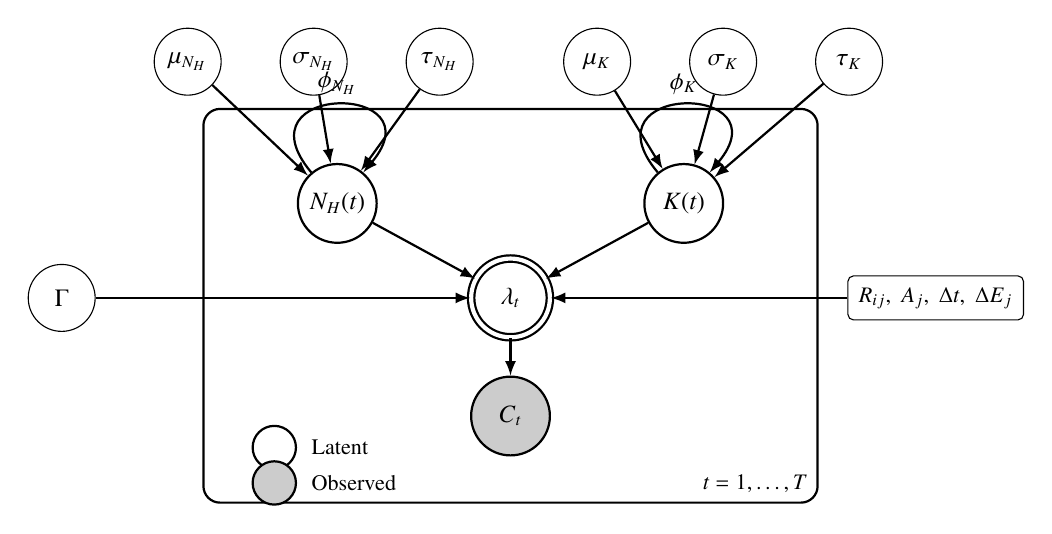
\begin{tikzpicture}[
    latent/.style={
        circle, draw=black, thick,
        minimum size=1.0cm, inner sep=0pt, font=\small},
    observed/.style={
        circle, draw=black, thick, fill=gray!40,
        minimum size=1.0cm, inner sep=0pt, font=\small},
    determ/.style={
        circle, draw=black, thick, double, double distance=1.5pt,
        minimum size=1.0cm, inner sep=0pt, font=\small},
    param/.style={
        circle, draw=black,
        minimum size=0.85cm, inner sep=0pt, font=\small},
    fixed/.style={
        rectangle, draw=black, rounded corners=2pt,
        inner sep=4pt, font=\footnotesize},
    arr/.style={-latex, thick}
]

%% ── Hyperparameters for N_H (outside plate) ─────────────────────
\node[param] (mu_nh)  at (0.0, 6.0) {$\mu_{N_H}$};
\node[param] (sig_nh) at (1.6, 6.0) {$\sigma_{N_H}$};
\node[param] (tau_nh) at (3.2, 6.0) {$\tau_{N_H}$};

%% ── Hyperparameters for K (outside plate) ───────────────────────
\node[param] (mu_k)  at (5.2, 6.0) {$\mu_K$};
\node[param] (sig_k) at (6.8, 6.0) {$\sigma_K$};
\node[param] (tau_k) at (8.4, 6.0) {$\tau_K$};

%% ── Spectral index (outside plate, left) ────────────────────────
\node[param] (gamma) at (-1.6, 3.0) {$\Gamma$};

%% ── Fixed instrument response (outside plate, right) ────────────
\node[fixed] (inst) at (9.5, 3.0)
    {$R_{ij},\; A_j,\; \Delta t,\; \Delta E_j$};

%% ── Plate ───────────────────────────────────────────────────────
\draw[thick, rounded corners=6pt]
    (0.2, 0.4) rectangle (8.0, 5.4);
\node[anchor=south east, font=\footnotesize]
    at (8.0, 0.4) {$t = 1, \ldots, T$};

%% ── Latent states (inside plate) ────────────────────────────────
\node[latent] (nh)  at (1.9, 4.2) {$N_H(t)$};
\node[latent] (k)   at (6.3, 4.2) {$K(t)$};

%% ── Expected count rate: deterministic (inside plate) ───────────
\node[determ] (lam) at (4.1, 3.0) {$\lambda_t$};

%% ── Observed photon counts (inside plate) ───────────────────────
\node[observed] (ct) at (4.1, 1.5) {$C_t$};

%% ── Arrows: hyperparameters → N_H(t) ────────────────────────────
\draw[arr] (mu_nh)  -- (nh);
\draw[arr] (sig_nh) -- (nh);
\draw[arr] (tau_nh) -- (nh);

%% ── Arrows: hyperparameters → K(t) ──────────────────────────────
\draw[arr] (mu_k)  -- (k);
\draw[arr] (sig_k) -- (k);
\draw[arr] (tau_k) -- (k);

%% ── AR(1) self-loops ─────────────────────────────────────────────
\draw[arr]
    (nh.130) .. controls +(130:1.5) and +(50:1.5) ..
    node[above, font=\small] {$\phi_{N_H}$}
    (nh.50);

\draw[arr]
    (k.130) .. controls +(130:1.5) and +(50:1.5) ..
    node[above, font=\small] {$\phi_K$}
    (k.50);

%% ── Arrows: N_H(t), K(t) → λ_t ──────────────────────────────────
\draw[arr] (nh) -- (lam);
\draw[arr] (k)  -- (lam);

%% ── Γ → λ_t ─────────────────────────────────────────────────────
\draw[arr] (gamma) -- (lam);

%% ── Instrument constants → λ_t ───────────────────────────────────
\draw[arr] (inst) -- (lam);

%% ── λ_t → C_t (Poisson emission) ────────────────────────────────
\draw[arr] (lam) -- (ct);

%% ── Legend ───────────────────────────────────────────────────────
\node[latent,  minimum size=0.55cm] (lg1) at (1.1, 1.1) {};
\node[right, font=\footnotesize] at (1.45, 1.1) {Latent};
\node[observed, minimum size=0.55cm] (lg2) at (1.1, 0.65) {};
\node[right, font=\footnotesize] at (1.45, 0.65) {Observed};

\end{tikzpicture}
\caption{Plate diagram of the hierarchical Bayesian state-space model.
Unshaded circles are latent random variables; the shaded circle
($C_t$) is the observed photon count; the double circle ($\lambda_t$)
is the deterministic expected count rate; small single circles are
inferred hyperparameters; the rectangle lists fixed instrument
quantities (RMF, ARF, exposure time, energy bin widths). The plate
encloses all quantities repeated over $T$ time steps. Curved
self-arrows indicate AR(1) temporal dependence with autocorrelation
coefficients $\phi_{N_H} = \exp(-1/\tau_{N_H})$ and
$\phi_K = \exp(-1/\tau_K)$.}
\label{fig:plate_diagram}
\end{figure*}

\begin{equation}
\begin{split}
p\!\left(\theta,\, \{N_H(t)\},\, \{K(t)\} \mid C\right)
\;\propto\;\;
& P(\theta)\cdot
p\!\left(\{N_H(t)\} \mid \theta\right) \\
&\cdot\;
p\!\left(\{K(t)\} \mid \theta\right)\cdot
\mathcal{L}\!\left(C \mid \theta,\,\{N_H(t)\},\,\{K(t)\}\right)
\end{split}
\label{eq:bayes}
\end{equation}
where $\theta = (\Gamma, \mu_{N_H}, \mu_K, \tau_{N_H},  \tau_K, \sigma_{N_H}, \sigma_K)$. The four terms on the right-hand side are the prior $P(\theta)$, the AR(1) structured priors on the latent trajectories $p(\{N_H(t)\} \mid \theta)$ and $p(\{K(t)\} \mid \theta)$, and the Poisson likelihood $\mathcal{L}(C \mid \theta, \{N_H(t)\}, \{K(t)\})$, respectively. First, we define a set of prior distributions over the parameters of interest (see Table~\ref{tab:priors}). \\

\begin{table}
\caption{Prior distributions of the model parameters.}
\label{tab:priors}
\centering
\begin{tabular}{lcc}
\hline\hline
Parameter & Distribution & Range / Parameters \\
\hline
$\Gamma$ & $\mathcal{U}$ & $[1.0,\,3.0]$ \\
$\mu_{N_H}$ & $\mathcal{U}$ & $[15.0,\,25.0]$ \\
$\mu_{K}$ & $\mathcal{U}$ & $[-6,\,-2]$ \\
$\ln \tau_{N_H}$ & $\mathcal{U}$ & $[\ln 2,\,\ln 80]$ \\
$\ln \tau_{K}$ & $\mathcal{U}$ & $[\ln 2,\,\ln 80]$ \\
$\sigma_{N_H}$ & $\mathcal{HN}$ & $0.5$ \\
$\sigma_{K}$ & $\mathcal{HN}$ & $0.5$ \\
\hline
\end{tabular}
\tablefoot{$\mathcal{U}$ denotes the uniform distribution and $\mathcal{HN}$ the half-normal distribution. Please note that the prior places uniform density on $\ln \tau_{N_H}$ and $\ln \tau_K$ over [$\ln 2$, $\ln 80$] which means $\tau_{N_H}$ and $\tau_K$ can range from 2 to 80 but are log-uniformly distributed, so that smaller values of $\tau_{N_H}$ and $\tau_K$ receive proportionally more prior probability than larger ones.}
\end{table}
The structured priors on the latent trajectories follow from the AR(1) state equation and are given by,
\begin{equation}
\begin{split}
p\!\left(\{N_H(t)\} \mid \theta\right)
= \;& p\!\left(N_H(1)\right) \\
&\times \prod_{t=2}^{T}
\mathcal{N}\!\left(N_H(t);\;
\mu_{N_H} + \phi_{N_H}\!\left(N_H(t-1)
- \mu_{N_H}\right),\;
\sigma_{N_H}^2\right)
\end{split}
\label{eq:ar1_prior_nh}
\end{equation}

\begin{equation}
p\!\left(\{K(t)\} \mid \theta\right)
= p\!\left(K(1)\right)
\prod_{t=2}^{T}
\mathcal{N}\!\left(K(t);\;
\mu_{K} + \phi_{K}\!\left(K(t-1) - \mu_{K}\right),\;
\sigma_{K}^2\right)
\label{eq:ar1_prior_k}
\end{equation}
where $\phi_{N_H} = \exp(-1/\tau_{N_H})$ and 
$\phi_K = \exp(-1/\tau_K)$. Next, we define the likelihood function as,

\begin{equation}
\mathcal{L}\!\left(C \mid \theta,\,\{N_H(t)\},\,\{K(t)\}\right)
= \prod_{t=1}^{T} \prod_{i=1}^{I}
\frac{\lambda_{ti}^{\,C_{ti}}\, e^{-\lambda_{ti}}}{C_{ti}!}
\label{eq:likelihood}
\end{equation}
where $C_{ti}$ is the observed photon count in detector channel $i$ at time step $t$, and the expected count $\lambda_{ti}$ (see Eq. \ref{eq:lambda_dis}). The full joint posterior in Eq.~\eqref{eq:bayes} is sampled using Hamiltonian Monte 
Carlo with the No-U-Turn Sampler (HMC/NUTS) as implemented in \textsc{NumPyro} \citep{phan2019composable}, which jointly infers $\theta$ and the latent trajectories $\{N_H(t)\}$ and $\{K(t)\}$ across all $T$ time steps. \\
We set the number of warm up steps to 2000 and the number of main samples to 6000. This way we ended up with 6000 posterior predictive samples. The inference was performed on a MacBook Pro with a 2.3 GHz 8-Core Intel Core i9 processor and 16 GB of memory. No graphic card was used. For a given $C_t$, the inference process, on average took $\approx 2$ hours. Table \ref{tab:light_curve_sim_table} shows the result of the inference for all the generated $C_t$s. \\

\subsection{Verification results}
\label{sec:verification_results}
In the following we present the results of the verification for both parameter recovery and the PSD recovery of the true data.\\
\subsubsection{Parameter recovery verification}
\label{sec:verification_results_parameter}
% Kozłowski (2017) ---> https://doi.org/10.1051/0004-6361/201629890
Earlier (Sect. \ref{sec:synthetic_data}) we used $\Gamma = 2$ as true value of the photon index. Looking at the fourth column of Table \ref{tab:light_curve_sim_table} we can see the model has been able to recover the correct value within two $\sigma$ very well for all the 26 count curves. The model also performs very well on $K$, $\sigma_{N_H}$ and $\sigma_K$. Across the 26 combinations, all these parameters were correctly inferred except the combination ($N_H = 20$, $\tau = 2$, $K = -3$) for $\sigma_{\tau}$. However, the model struggles to perform over $N_H$ as well as it did over $K$. Of the 26 $C_t$s, the model was not able to recover the parameters for seven of them (see Table \ref{tab:nh_failures}). Of these seven misses, three of them are marginal misses, and a rounding effect could be the possible explanation. Another point to note is that of all the $C_t$s with $N_H = 19$, three of them are among the ones that our model was not able to recover $N_H$ correctly. This behaviour is the result of degeneracy at low $N_H$. In other words, looking at optical depth for different values of $N_H$ the photon absorption rate for $N_H = 10^{19}$ is almost the same as, for instance, $N_H = 10^{16}$ or $N_H = 10^{10}$ (read Appendix \ref{app:optical_depth} and see Fig. \ref{fig:nh_flux_threshold} for further details). This means at the low $N_H$ regime the data carry very little information about $N_H$, causing HMC to explore $N_H$ values that are much smaller than the original $N_H = 10^{19}$ and shifting the posterior toward smaller values of $N_H$ (see Fig. \ref{fig:nh_posterior_degeneracy}). Another point worth mentioning is that among the four combinations with $N_H = 19$ the one that has been correctly recovered is the one with the lowest photon count. Looking at the posterior distribution of this combination, it is similar to Fig. \ref{fig:nh_posterior_degeneracy} with a longer tail toward higher values of $N_H$. This indicates that the lower count leads to higher ambiguity of HMC and, in turn, a heavier tail. This means the capture of the true value of $N_H$ in this combination is not the result
of information extracted from the data. The posterior median lies at
$\log_{10} N_H = 17.25$, nearly two decades below the true value, and the true value
falls inside the $5\%$--$95\%$ credible interval only because that interval spans more
than four decades ($15.0$--$19.2$), entering $0.2$ dex below its upper edge. The three
$N_H = 19$ combinations counted as failures miss by a comparable margin from intervals
of similar width. At this column density the posterior is essentially uninformative, and
containment of this kind should not be read as a detection. Table \ref{tab:nh_failures} therefore understates the difficulty at this column density. The fourth $N_H = 19$ combination is excluded from it only because it formally satisfies
the $5\%$--$95\%$ containment criterion, and we regard the effective failure rate at
$N_H = 19$ as four out of four. \\
Finally, we take a look at $\tau_{N_H}$ and $\tau_K$. At first, it looks like all but one $\hat\tau_{N_H}$ and one $\hat\tau_K$ for ($N_H = 22$, $\tau = 50$, $K = -4$) and ($N_H = 21$, $\tau = 50$, $K = -3$) combinations, respectively, were not correctly inferred. However, these results are misleading. A closer look at the $\hat\tau_{N_H}$ and $\hat\tau_K$ columns reveals that for some combinations the credible intervals are quite large. This shows that HMC has not been able to pin down the true value well. Fig. \ref{fig:tau_posterior_Nh22_Tau38_phi-4} shows the prior and posterior comparison for both $\hat\tau_{N_H}$ and $\hat\tau_K$ for combination ($N_H = 22$, $\tau = 38$, $K = -4$) which shows a large credible interval. It is clear that the posterior has learned very little from the data. There are two further observations that could help us in explaining the inability of HMC in pinning down the true value. The first point to note is that as we move from $N_H = 19$ to $N_H = 24$, we can see that the credible interval for $\hat\tau_{N_H}$ tends to stay quite large for true values of $\tau_{N_H} = 38$ and $\tau_{N_H} = 50$ while the credible interval decreases for $\tau_{N_H} = 2$. The second point to note is that $\hat\tau_K$ shows a similar behaviour except that even at $\tau = 2$ the credible interval for $\hat\tau_K$ remains small. According to \citet{Kozlowski2017}, the observed pattern in $\hat\tau_{N_H}$ and $\hat\tau_K$ is expected. \citet{Kozlowski2017} found that in modelling the light curve of AGNs with a DRW process, in order to correctly recover the timescale parameter, $\tau$, the length of the observation, $t$, must be at least ten times larger ($t \ge 10 \tau$; see Fig. 2 of \citealt{Kozlowski2017}). We remind the reader that our $C_t$s run for one hundred time steps. Therefore, the largest value of $\tau$ we can estimate is $\tau \le 10$. This explains why our model was not able to pin down the posterior distribution of $\tau$ when $\tau = 38$ and $\tau = 50$ as it requires $C_t$s with lengths at least as long as $\approx 400$ and $\approx 500$ time steps, respectively. Contrary to $\tau = 38$ and $\tau = 50$, our model should be able to recover $\tau = 2$ well. Indeed, our model is able to recover $\tau_K$ when $\tau = 2$; however, it fails in recovering $\tau_{N_H}$. The likely explanation lies in the geometry of the parameter space that HMC has to explore. Looking at equations \ref{eq:zpowerlaw} and \ref{eq:zwabs}, parameters $K$ and $N_H$ enter the picture in a linear and non-linear fashion, respectively. The fact that $N_H$ is an exponent of the exponential function and its impact on different energy channels is different (due to Wisconsin cross-section) makes the parameter space more complex for HMC to explore, yielding a less reliable estimate of $\tau_{N_H}$. The inability of our model in estimating the true distribution of $\tau_{N_H}$ at $\tau = 2$ requires further investigation. \\

\begin{table}[htbp]
\caption{Combinations where $N_H$ was not recovered within the 
5\%--95\% posterior credible interval.}
\label{tab:nh_failures}
\centering
\begin{tabular}{ccc}
\hline\hline
$N_H$ & $\tau$ & $K$ \\
\hline
19 & 2  & $-4$ \\
19 & 38 & $-4$ \\
19 & 50 & $-4$ \\
20 & 2  & $-3$ \\
20 & 50 & $-3$ \\
22 & 38 & $-4$ \\
22 & 50 & $-3$ \\
\hline
\end{tabular}
\tablefoot{Three entries ($N_H=19/\tau=38$, $N_H=20/\tau=2$, 
$N_H=22/\tau=50$) are marginal misses of 0.03, 0.02, and 0.01, 
respectively.}
%, likely attributable to rounding in the reported 
%credible interval bounds.}
\end{table}


\begin{figure}[htbp]
\centering
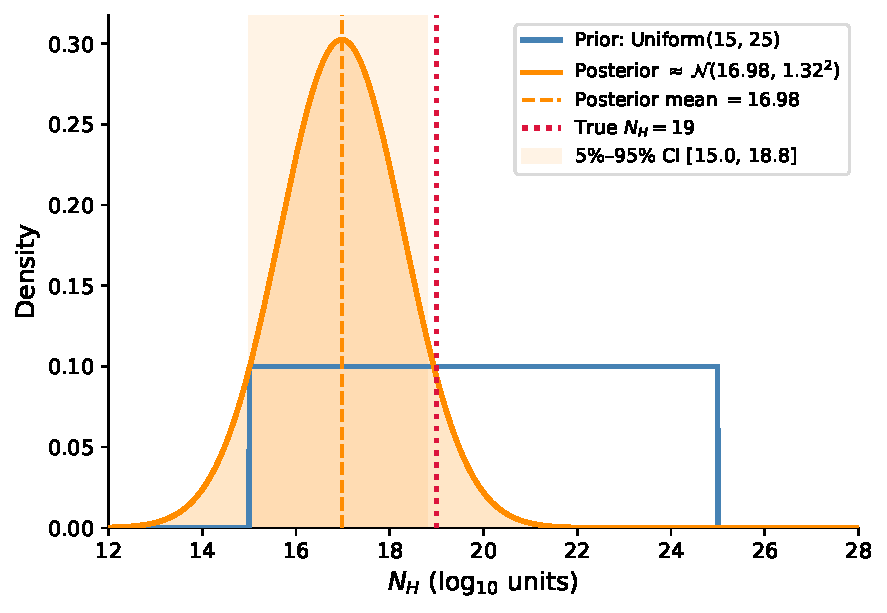
\includegraphics[width=\columnwidth]{nh_posterior_Nh19_Tau2_phi-4_paper.pdf}
\caption{Prior and posterior distribution of the hydrogen column
density $N_H$ for the simulation with true $N_H = 10^{19}$\,cm$^{-2}$,
$\tau = 2$, and $K = -4$. The flat blue curve is the assumed
uniform prior over $[15, 25]$ in $\log_{10}$ units. The orange curve
is the inferred posterior, approximated by a Gaussian with mean
$\hat{N}_H = 16.98$ and standard deviation $1.32$; the shaded orange
band marks the 5\%--95\% credible interval $[15.0,\,18.8]$, which
does not include the true value (red dotted line at $N_H = 19$).
The systematic shift of the posterior toward lower values is a direct
consequence of the absorption degeneracy illustrated in
Fig.~\ref{fig:nh_flux_threshold}. At $N_H \lesssim 10^{20}$\,cm$^{-2}$
the photoelectric attenuation factor $e^{-N_H\sigma(E)} \approx 1$
across the entire observed energy band, making the photon count
time series insensitive to the exact value of $N_H$. Any column
density below $\sim\!10^{20}$\,cm$^{-2}$ produces an effectively
identical observed spectrum, so the likelihood is nearly flat in
this regime and the posterior drifts toward the lower end of the prior.}
\label{fig:nh_posterior_degeneracy}
\end{figure}

\begin{figure}[htbp]
    \centering
    
\includegraphics[width=\columnwidth]{tau_posterior_Nh22_Tau38_phi-4_paper.pdf}
    \caption{Prior and posterior distributions of the AR(1) timescale parameters
             for the simulation with $N_H = 10^{22}$~cm$^{-2}$, $\tau = 38$ time steps,
             and $K = -4$.
             In both panels the blue curve shows the log-uniform prior
             $p(\tau) \propto \tau^{-1}$ on $\tau \in [2, 80]$ time steps, the orange
             curve and shaded region show the Log-Normal posterior approximation,
             the orange dashed line marks the posterior median, the red dotted
             line marks the true value of $\tau$ (38 time steps), and the light
             orange band spans the 5\%--95\% credible interval.
             \emph{Top:} Posterior of the column-density timescale $\tau_{N_H}$.
             The posterior median is 21.1 time steps with a 5\%--95\% credible interval
             of $[7.1,\,77.5]$ time steps; the true value lies within the interval but
             the posterior is biased toward shorter timescales, reflecting the
             limited number of effective correlation lengths ($T/\tau \approx 2.6$)
             available in the $T = 100$-step light curve.
             \emph{Bottom:} Posterior of the flux-normalisation timescale
             $\tau_K$.  The posterior median is 34.5 time steps with a 5\%--95\%
             credible interval of $[15.8,\,80.0]$ time steps; the true value is again
             recovered within the interval and the posterior is narrower
             ($\sigma_{\ln\tau} = 0.54$ versus $0.77$ for $\tau_{N_H}$), indicating
             that the flux-normalisation process is better constrained by the data
             than the column-density process for this parameter combination. However, in both cases the posterior is almost as broad as the prior.}
    \label{fig:tau_posterior_Nh22_Tau38_phi-4}
\end{figure}



\subsubsection{PSD recovery verification}
\label{sec:verification_results_psd}
In Sect. \ref{sec:verification_results_parameter} we checked the performance of our model
over the suite of ground-truth $C_t$s. Now, a more important question to answer is
whether our model has been able to recover their true temporal dependence. In other words, whether it recovers their true PSD. Before turning to these light curves, we
first tested our model on a simpler set of $C_t$s that were generated based on a simple
colour-noise process with PSD function of the form $\propto f^{-\beta}$ with $\beta = \{1.7, 3, 4\}$. This data set does not take into account the absorption and instrumental response matrices (see Appendix \ref{app:recovery} for more details on the light curve generation, inference, and fitting procedure). Running our model over this data set, we found the true $\beta$ falls outside the recovered [5\%-95\%] credible interval for all three cases. For $\beta = 1.7$ this is consistent with ordinary realisation-to-realisation scatter of the periodogram estimator rather than a systematic recovery bias; for $\beta = 3$ and $\beta = 4$ it instead reflects a systematic bias of the periodogram fit, whose limited dynamic range caps the steepest slope recoverable across the binned frequency range (Appendix~\ref{app:recovery}). \\
Next, we tested the capability of our model in recovering the true PSD of the $C_t$s we generated in Sect. \ref{sec:synthetic_data}. As we described earlier we used a posterior sample size of 6000. This means for each $N_H$, $\tau$ and $K$ combination (see Table \ref{tab:light_curve_sim_table})
we have 6000 inferred $C_t$s that share the same statistical properties as the
ground-truth $C_t$. For each combination, we estimate the periodogram of the
ground-truth $C_t$. Next, we bin the periodogram according to \citet{Vaughan2003}. Finally, we fit the binned data to the power-law function of the form

\begin{equation}
\label{eq:periodogram_fit}
    \log(P) = \log\left(a f^{-\beta} + c\right),
\end{equation}
where $f$ is frequency and $P$ is the value of periodogram at that frequency and $a$, $\beta$, and $c$ are to be estimated. We follow the same steps for each posterior sample of that specific combination until we have six thousand $\beta$ values. Fig. \ref{fig:psd_beta_recovery_tau2} shows the entire process for the combination $N_H = 21$, $\tau = 2$, $K = -3$. In the upper row of Fig. \ref{fig:psd_beta_recovery_tau2} shows the true and posterior samples of the $N_H$ and $K$ processes. The middle row shows the binned true PSD and posterior samples along with the best fits. The posterior sample fits closely follow the true fit in both plots. \\
In the bottom row of Fig. \ref{fig:psd_beta_recovery_tau2}, we have provided the distribution of the recovered $\beta$ values each from fitting a posterior sample. It is clear that the true $\beta$ falls within the [5\% - 95\%] credible interval. Also, a notable feature is the heavy tail of the $\beta$ distribution in the bottom left plot. This heavy tail has shifted the credible interval towards higher values. \\
We further investigate the possible explanations for the observed heavy tail in the $\beta_{N_H}$ distribution. We extracted three of the posterior samples for which $\beta_{N_H} \ge 4$. The processes and their PSD fit are shown in Fig. \ref{fig:nh_extreme_comparison}. According to Fig. \ref{fig:nh_extreme_comparison} the main reason behind the observed heavy tail is the short duration of $C_t$ while the binning exacerbates it. The short duration causes the first few bins of PSD to have only a few data points. Given PSD follows a $\chi^2$ distribution of second degree the variance can vary $100\%$ for the bins with only one data point in them and the variance decreases as the number of points in a bin increases. This means the first bin can vary widely. This is visible in the right plot of the middle row of Fig. \ref{fig:psd_beta_recovery_tau2} where the first bin, with one data point, shows a sudden drop in power compared to the second bin, with more than one data point. The same reasoning can be used to explain the small bump at higher values in the distribution of $\beta$. Looking at the bottom row of Fig. \ref{fig:nh_extreme_comparison} one can see the fit goes through the first two bins and then it flattens. This is because in these particular instances the first two bins have lower variance compared to the bins at higher frequencies. This in turn causes the fitting algorithm to assign a larger weight to the first bins. For instance, for the process with index 382, the second bin contains only two data points and they happen to be very similar. This produces a very small variance, which in turn makes the second bin act as an anchor for the fit while the rest of the bins have a much smaller weight in this process. The slope of the power law is very dependent on the first two bins in these extreme cases. This is especially visible in the middle plot (index 219) in bottom row of Fig. \ref{fig:nh_extreme_comparison} where the first bin falls at the upper end of the credible interval while the second bin falls at the bottom of the credible interval. This leaves the optimiser with no choice but to assign a steep slope ($\beta = 4.48$) to connect the two bins. A similar explanation applies to the right plot in the bottom row of Fig. \ref{fig:nh_extreme_comparison}. These extreme cases all arise to varying extent from an unusually high $\chi^2(2)$ draw at the single periodogram point in the lowest-frequency bins (see Fig. \ref{fig:nh_extreme_comparison} caption for details). \\
For the extreme cases shown in Fig. \ref{fig:nh_extreme_comparison}, the free
parameter $c$ takes values of $\approx 0.1$, while its median value across the posterior
samples is $\approx 0.005$ (see App. \ref{app:recovery} for more details). This means for the majority of the posterior samples the fit is smooth and the power law is the dominant component while the flattening takes over at frequencies higher than the observed range of frequencies in Fig. \ref{fig:psd_beta_recovery_tau2} and \ref{fig:nh_extreme_comparison}. It should be emphasised that the parameter $c$ is important to keep, as removing it from the fit will result in flatter $\beta$ estimates. This happens because the algorithm tries to fit one power law to all the bins at once. In addition, $c$ has physical interpretation and captures the flattening at the higher frequencies where the Poisson noise, red-noise power leakage, and intrinsic flattening of PSD of AR(1) dominate the power law, similar to the constant term used by \citet{Alston2019} to account for the Poisson-noise plateau in their PSD fitting (see App. \ref{app:recovery} for more details). \\
We stated the reason behind the small bump at higher $\beta$ values is the binning of a short process, which leaves the first few bins with very few data points and, in turn, causes the first few bins to vary significantly. This means if we can reduce the variance in these bins by adding more points to them we should be able to reduce the number of extreme $\beta$ values and removing the observed bump at higher values in the $\beta$ distribution. To test our reasoning we generated $C_t$ curves with the same combination of $N_H = 21$, $\tau = 2$, $K = -3$ but for 500 time steps instead of 100 and we performed the same inference process. Looking at the bottom left plot of Fig. \ref{fig:psd_beta_recovery_tau2_t500} we can see two things happening at the same time. First, the second bump at higher values of $\beta$ is gone. Second, the $\beta$ distribution has become tighter. The disappearance of the small bump at higher values of the $\beta$ distribution and the tightening of the $\beta$ distribution is expected as there are more data points in each bin, which in turn means less variance in each bin. This is especially visible in the left plot of the middle row in Fig. \ref{fig:psd_beta_recovery_tau2_t500}. The grey shaded area is tighter at lower frequencies and it becomes even tighter at higher frequencies. This tightening of the grey shaded area creates less extreme values of the power in each bin, especially in the first few bins. Consequently, there are less extreme cases of large $\beta$ values and a tighter distribution around the true value of $\beta$. \\
A more interesting change is that the true value of $\beta$ has shifted from 1.27 to 0.72. In other words, $\beta$ has become significantly flatter. Looking at the middle row of Fig. \ref{fig:psd_beta_recovery_tau2_t500} we can see more bins fall on the frequency range smaller than $f_{bend}$. Thus, a fit to these bins yields flatter $\beta$ values. Given we kept $\tau_{N_H} = 2$ and increased $T$ to $500$, this shows as $T/\tau$ increases more bins fall on the frequency range $f \le f_{bend}$, which in turn drives flatter $\beta$ values. This is true for both $N_H(t)$ and $K(t)$. This makes the interpretation of the $\beta$ values recovered by our model complicated. In other words, one cannot be sure of the recovered $\beta$ unless there is some estimation of $\tau$ (see Sect. \ref{sec:limitation}). \\ 

\begin{figure*}[htbp]
    \centering
    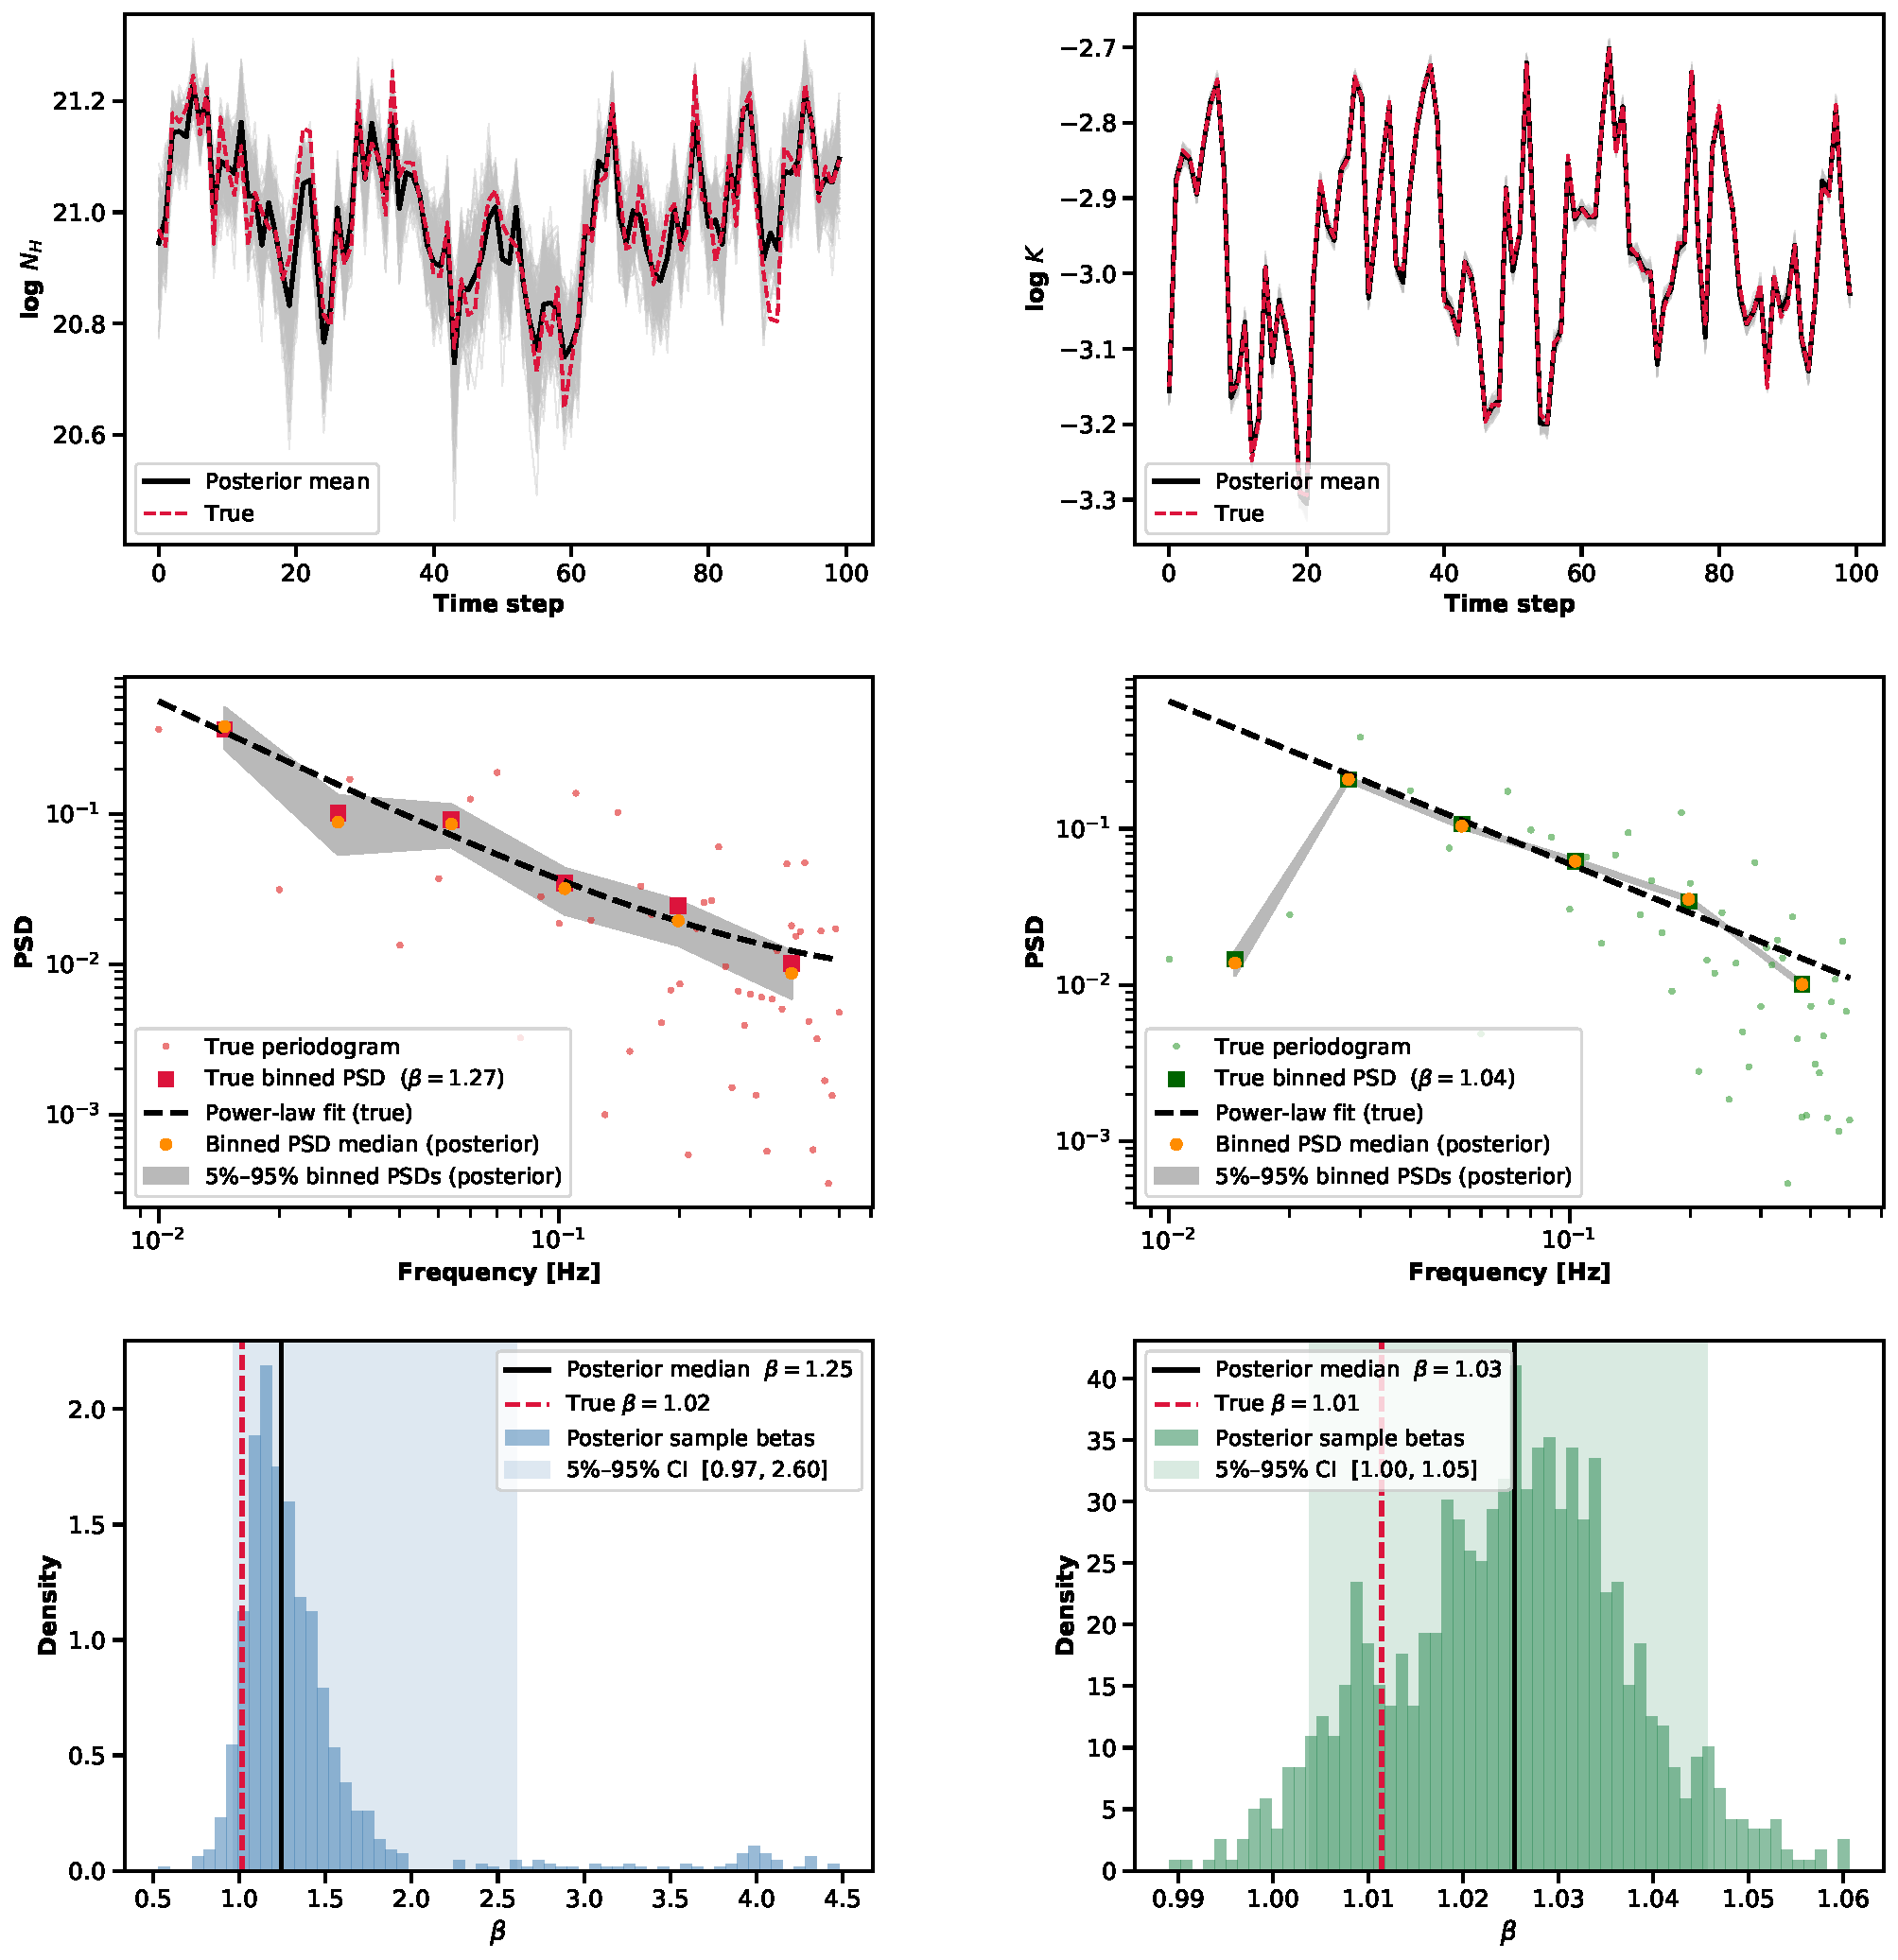
\includegraphics[width=\textwidth]{psd_beta_recovery_Nh21_Tau2_Phi-3_methodB_paper.pdf}
    \caption{PSD recovery for the parameter
    combination $\log N_H = 21$, $\tau = 2$, $\log K = -3$.
    \emph{Top row:} Posterior time-series reconstruction for the $\log N_H$ process
    (left) and the $\log K$ process (right). Light grey traces show 200 individual
    posterior samples; the solid black line is the posterior mean; the dashed red
    line is the true (generating) time series.
    \emph{Middle row:} PSD panels for the $\log N_H$ process (left) and the $\log K$
    process (right). The grey shaded band spans the 5th–95th percentile of the
    1000 posterior-sample binned PSDs. True periodogram points are shown in red (left)
    and green (right); true binned PSD values are marked with filled squares 
    (red left, dark green right). The black dashed line is the
    power-law fit to the true binned PSD. Orange circles mark the median of the
    posterior binned PSDs. The vertical dashed line shows the location of the bend frequency ($f_b$).
    \emph{Bottom row:} Distribution of the power-law index $\beta$ recovered from
    individual posterior-sample periodograms for $\log N_H$ (left, blue)
    and $\log K$ (right, green). The shaded band indicates the 5th–95th percentile
    credible interval; the solid black vertical line marks the posterior median; the
    dashed red line marks the true $\beta$ derived from the generating time series.
    For $\tau = 2$ both processes are recovered well, with the posterior $\beta$
    distribution centred close to the true value.}
    \label{fig:psd_beta_recovery_tau2}
\end{figure*}


\begin{figure*}[htbp]
    \centering
    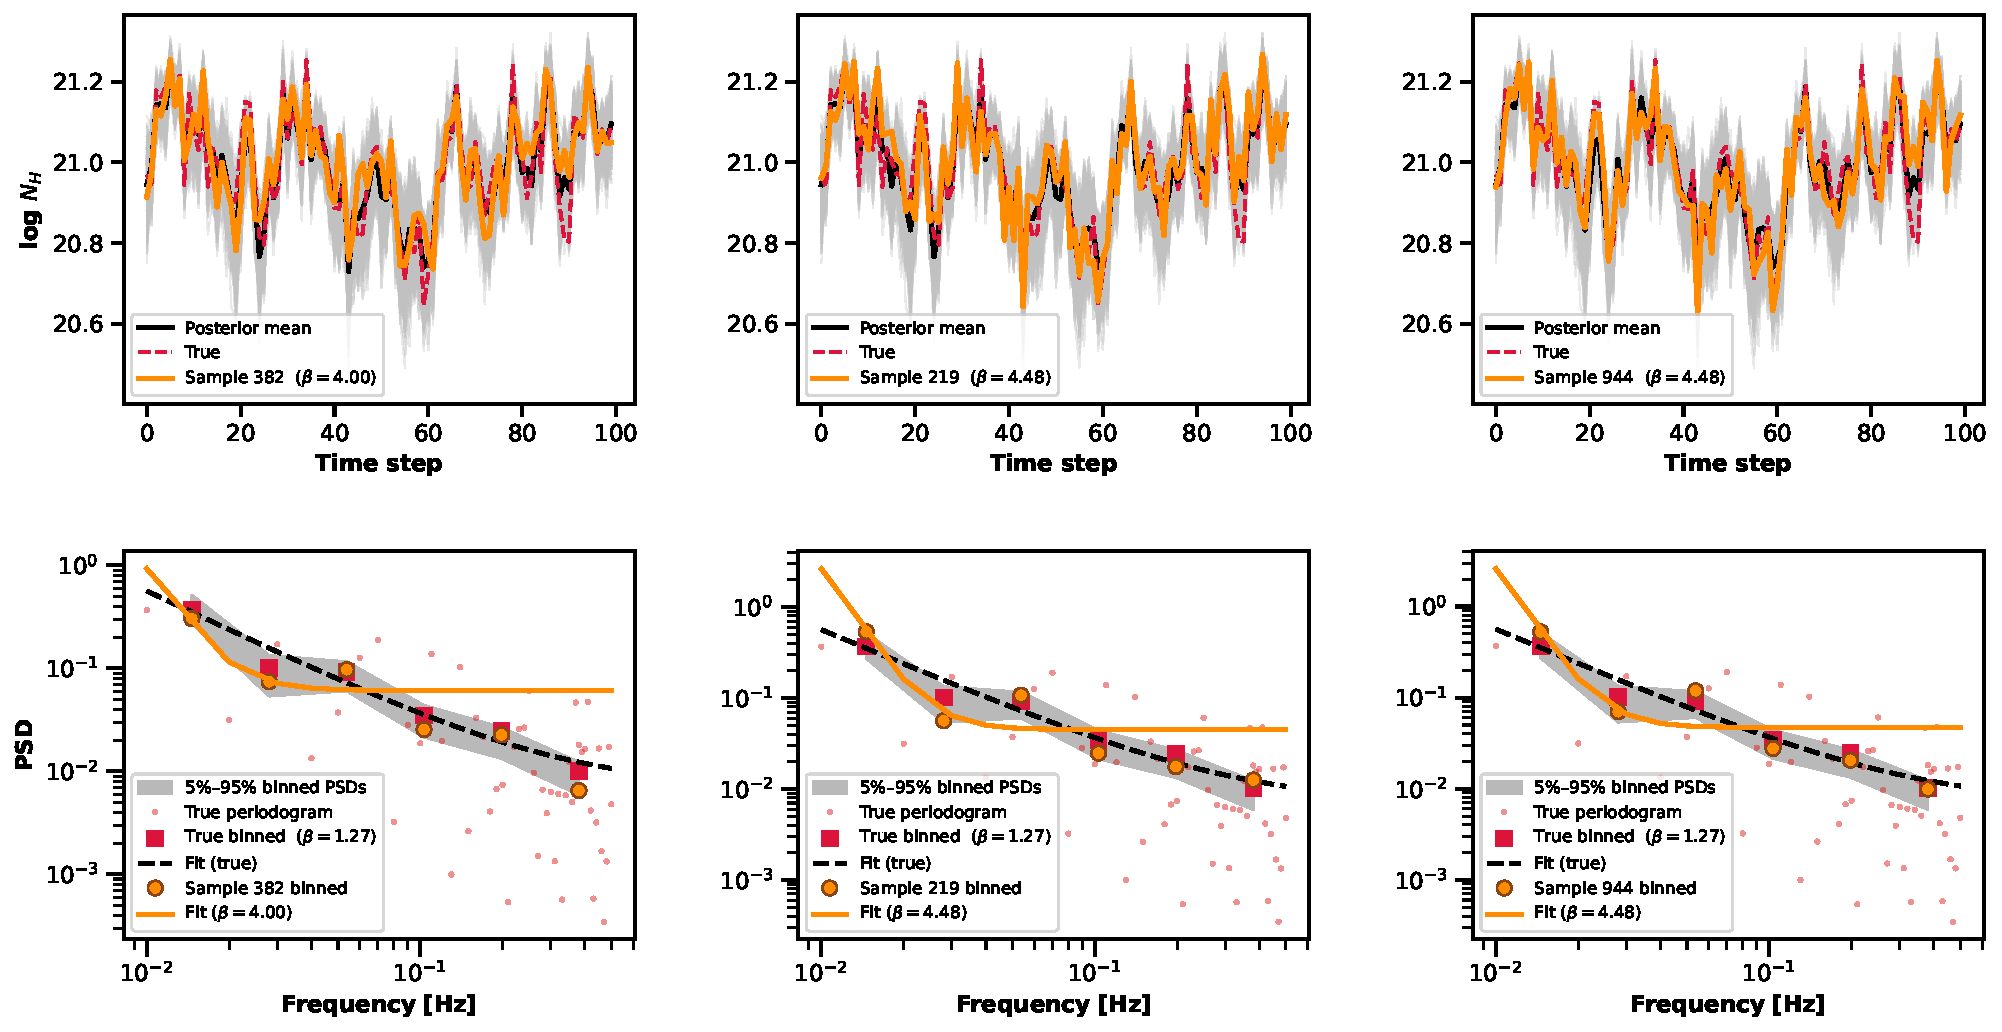
\includegraphics[width=\textwidth]{nh_extreme_comparison_Nh21_Tau2_Phi-3_v2.pdf}
    \caption{Diagnostic comparison of three extreme-$\beta$ posterior samples of
    the $\log N_H$ process for the parameter combination
    $\log N_H = 21$, $\tau = 2$, $\log K = -3$.
    \emph{Top row:} Corresponding $\log N_H$ time series.
    Silver traces: 50 randomly selected posterior samples; black solid line:
    posterior mean; red dashed line: true generating trajectory;
    orange line: the highlighted sample.
    \emph{Bottom row:} 
    PSD for each sample.
    Grey shaded band: 5th--95th percentile of all 1000 posterior binned PSDs.
    Red dots and red squares: true periodogram and binned PSD
    ($\beta_\mathrm{true} = 1.27$); black dashed line: true power-law fit.
    Orange circles: the sample's binned PSD;
    orange solid line: power-law fit to that sample.
    \emph{Left column} (sample 382, $\beta=4.00$): bin~1 sits \emph{below} the
    true spectrum yet $\beta=4$ is reported, a fitting artefact caused by
    bin~2 having near-zero within-bin variance (two nearly identical periodogram
    points), which collapses its sigma weight to ${\sim}4250$ and forces the
    power-law fit to anchor at bin~2, yielding a spuriously steep slope.
    \emph{Middle and right columns} (samples 219 and 944, $\beta \approx 4.48$):
    bin~1 sits visibly above the true spectrum, consistent
    with a high draw from the $\chi^2(2)$ distribution at the single periodogram
    point in the lowest-frequency bin.
    In all three cases the artefact originates from the short time series
    ($T=100$), which leaves only one periodogram point in bin~1 and at most two
    in bin~2, making the low-frequency anchor of the power-law fit highly
    unstable.}
    \label{fig:nh_extreme_comparison}
\end{figure*}


\begin{figure*}[htbp]
    \centering
    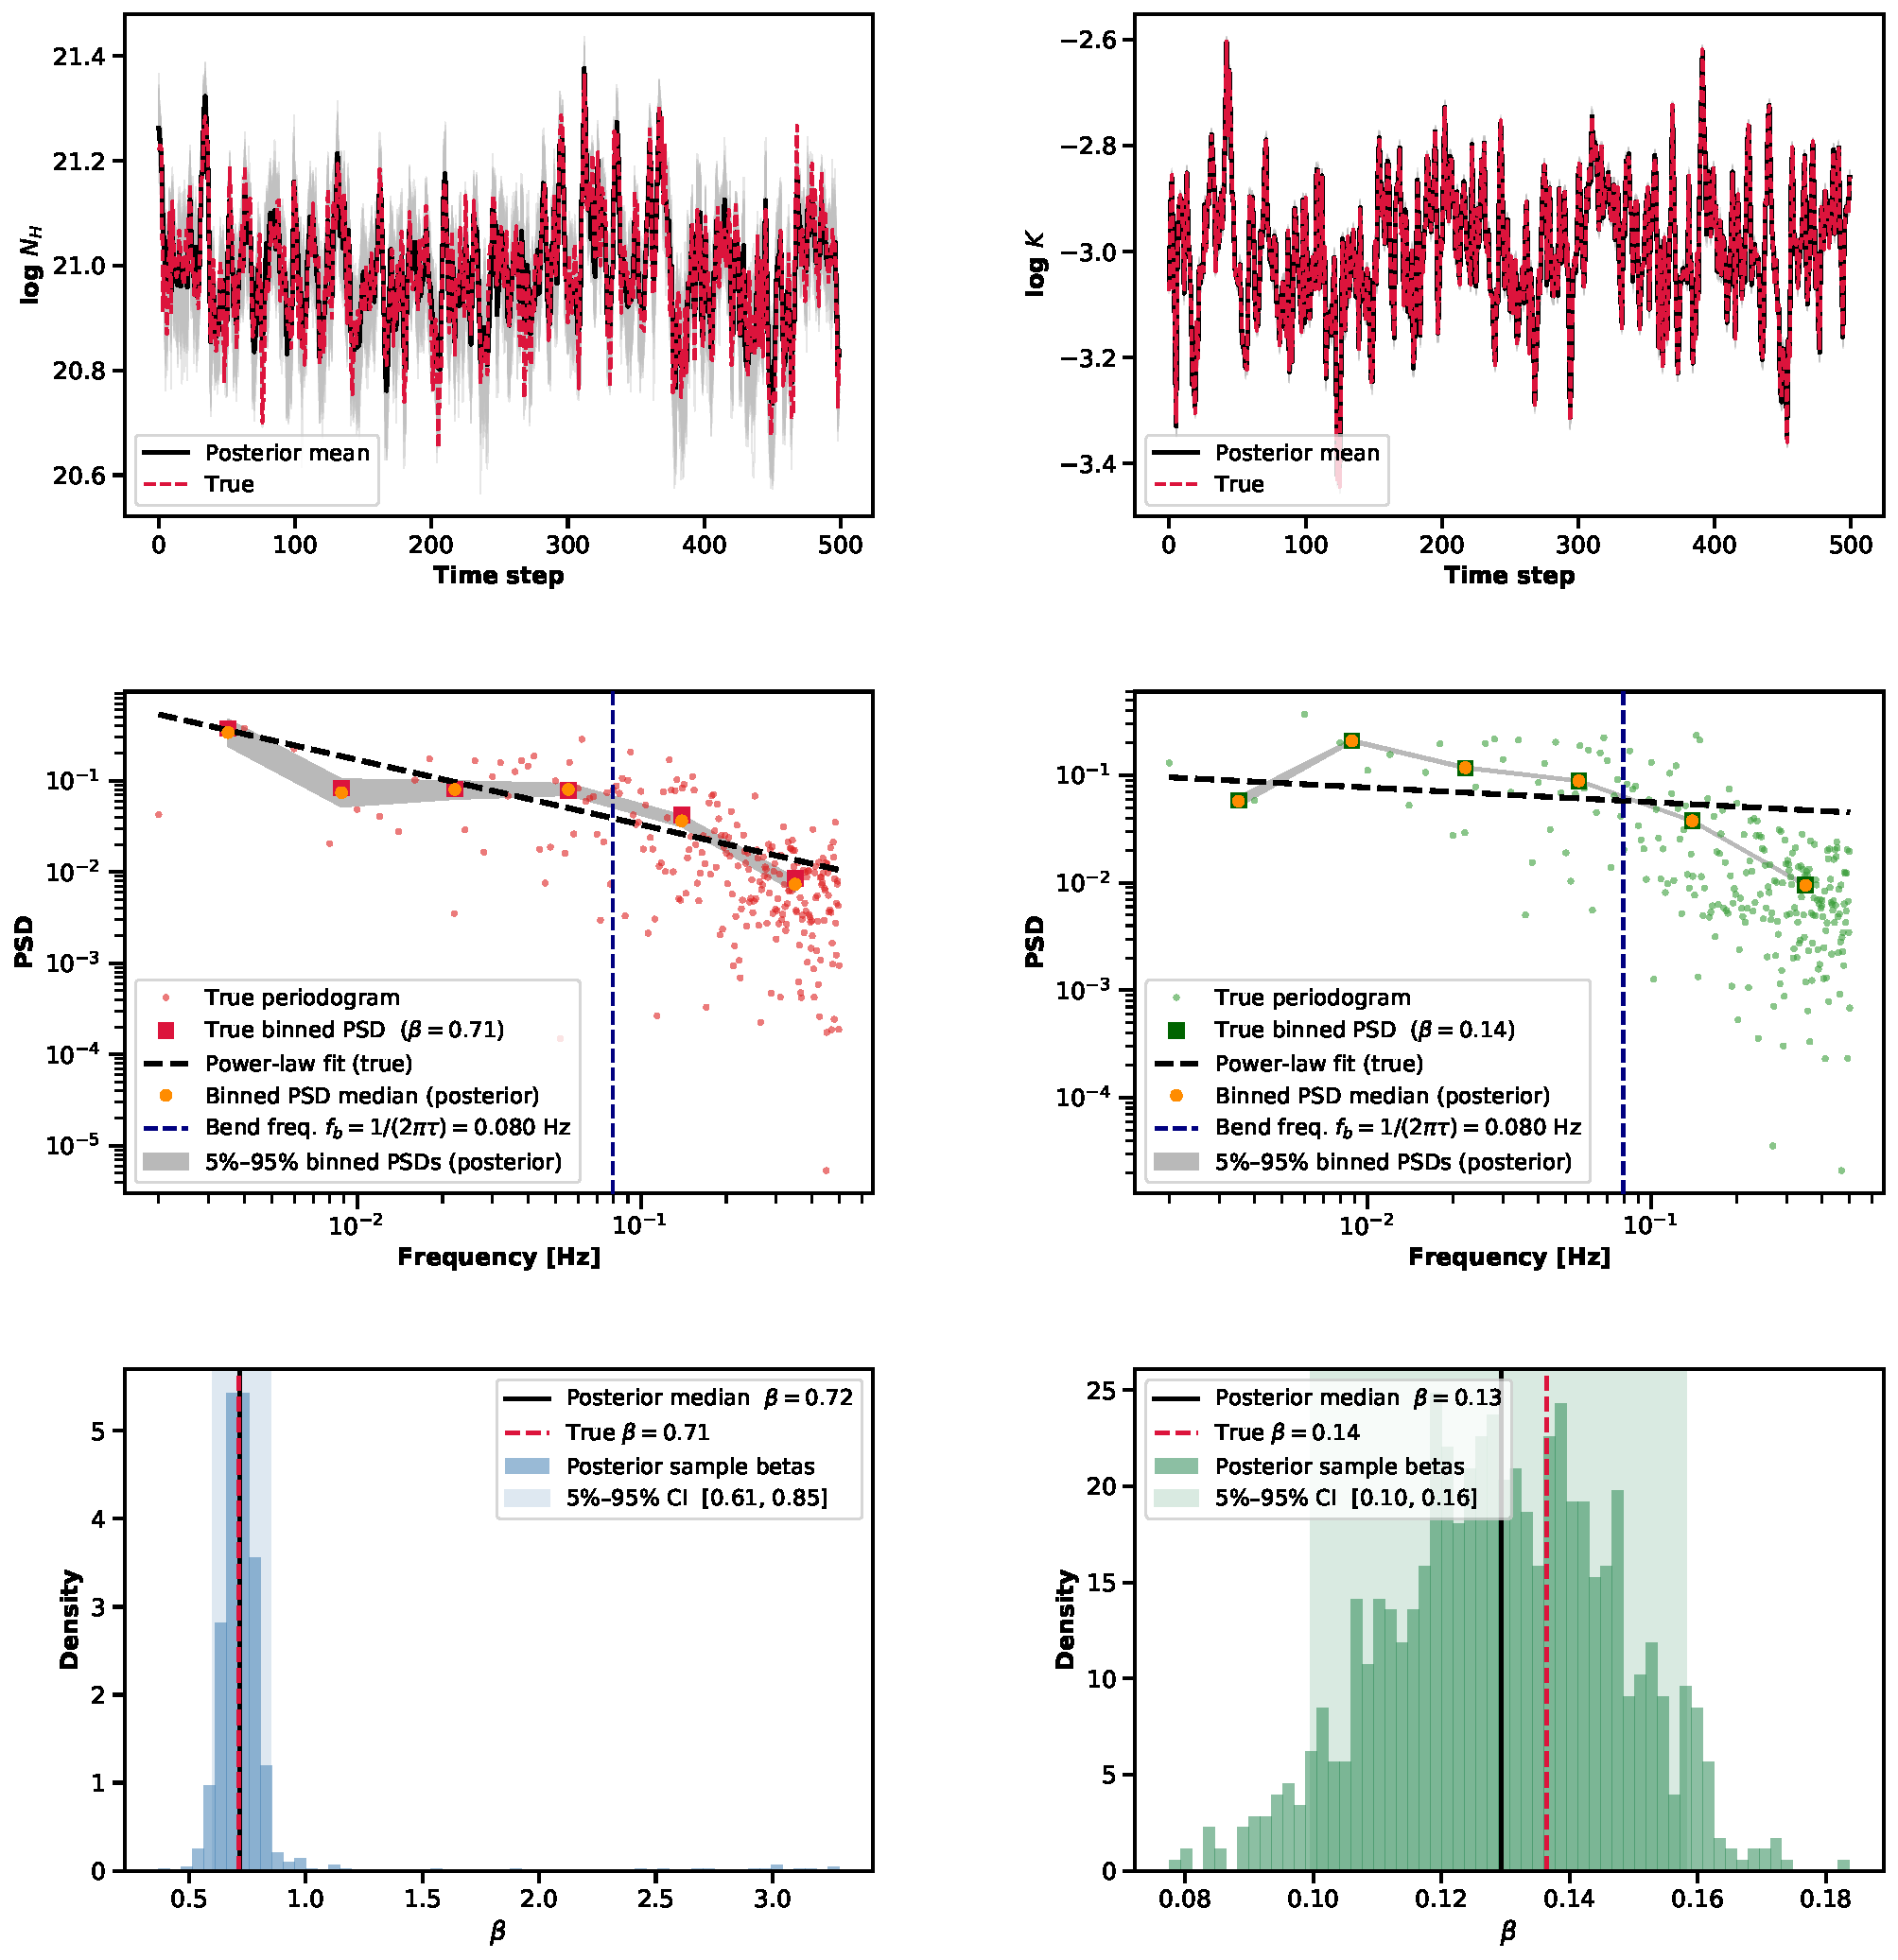
\includegraphics[width=\textwidth]{psd_beta_recovery_Nh21_Tau2_Phi-3_T500_methodB_withC_fixed.pdf}
    \caption{PSD recovery for the parameter
        combination $\log N_H = 21$, $\tau = 2$, $\log K = -3$ with an
        extended time series of $T = 500$ steps (cf.\ Fig.~\ref{fig:psd_beta_recovery_tau2}
        for the $T = 100$ case).
        \emph{Top row:} Posterior time-series reconstruction for the $\log N_H$ process
        (left) and the $\log K$ process (right). Light grey traces show 200 individual
        posterior samples; the solid black line is the posterior mean; the dashed red
        line is the true (generating) time series.
        \emph{Middle row:} PSD panels for the $\log N_H$ process (left) and the $\log K$
        process (right). The grey shaded band spans the 5th–95th percentile of the
        1000 posterior-sample binned PSDs. True periodogram points are shown in red (left)
        and green (right); true binned PSD values are marked with filled squares
        (red left, green right). The black dashed line is the
        power-law fit to the true binned PSD. Orange circles mark the median of the
        posterior binned PSDs. Compared to $T = 100$, the additional frequency resolution
        shifts several bins below the break frequency $f_b \approx 0.08$\,cycles\,step$^{-1}$ (the vertical dashed line). 
        The power-law fit must now
        balance bins from both the flat and power-law regimes, which drives the recovered
        $\beta$ to lower values than in the $T = 100$ case.
        \emph{Bottom row:} Distribution of the power-law index $\beta$ recovered from
        individual posterior-sample periodograms for $\log N_H$ (left, blue)
        and $\log K$ (right, green). The shaded band indicates the 5th–95th percentile
        credible interval; the solid black vertical line marks the posterior median; the
        dashed red line marks the true $\beta$ derived from the generating time series.
        Compared to $T = 100$, the credible interval is substantially narrower and the
        heavy tail toward large $\beta$ is strongly suppressed, a direct consequence of
        the larger number of periodogram points per frequency bin which stabilises the
        bin estimates and reduces the leverage of individual outlier bins on the
        power-law fit.}
    \label{fig:psd_beta_recovery_tau2_t500}
\end{figure*}


\begin{table*}
        \caption{Light curve simulations and parameter recovery under different $N_H$, $\tau$, and $K$ values}
        \label{tab:light_curve_sim_table}
        \centering
        \begin{tabular}{lcccccccccc}   % <- change number of c's to M columns
        \hline\hline
        $N_H$ & $\tau$ & $K$ & $\hat\Gamma$ & $\hat{N_H}$ & $\hat\tau_{N_H}$ & $\hat K$ & $\hat\tau_K$ & $\hat\sigma_{N_H}$ & $\hat\sigma_K$ & count \\
        \hline
        19 & 2 & -4 & $2.001 \pm 0.013$ & $16.98^{+1.80}_{-1.98}$ & $12.1^{+87.5}_{-10.6}$ & $-3.99^{+0.06}_{-0.05}$ & $2.4^{+1.0}_{-0.7}$ & $0.337 \pm 0.491$ & $0.110 \pm 0.017$ & 96,829 \\
        19 & 2 & -5 & $2.021 \pm 0.040$ & $17.25^{+1.97}_{-2.24}$ & $11.2^{+82.5}_{-9.9}$ & $-4.97^{+0.07}_{-0.06}$ & $3.0^{+2.6}_{-1.4}$ & $0.335 \pm 0.490$ & $0.115 \pm 0.020$ & 10,273 \\
        19 & 38 & -4 & $1.991 \pm 0.013$ & $17.08^{+1.89}_{-2.08}$ & $11.9^{+88.5}_{-10.5}$ & $-4.15^{+0.51}_{-0.46}$ & $39.5^{+54.9}_{-23.0}$ & $0.321 \pm 0.504$ & $0.092 \pm 0.015$ & 93,868 \\
        19 & 50 & -4 & $2.001 \pm 0.015$ & $17.07^{+1.83}_{-2.07}$ & $11.7^{+85.0}_{-10.3}$ & $-4.23^{+0.56}_{-0.50}$ & $37.2^{+60.3}_{-23.0}$ & $0.328 \pm 0.496$ & $0.103 \pm 0.016$ & 79,036 \\
        20 & 2 & -3 & $2.004 \pm 0.007$ & $20.12^{+0.11}_{-0.10}$ & $8.7^{+63.3}_{-7.6}$ & $-2.99^{+0.05}_{-0.05}$ & $2.3^{+0.7}_{-0.5}$ & $0.023 \pm 0.042$ & $0.104 \pm 0.015$ & 939,181 \\
        20 & 2 & -4 & $2.000 \pm 0.025$ & $18.64^{+1.70}_{-2.83}$ & $9.7^{+60.3}_{-8.3}$ & $-4.00^{+0.06}_{-0.06}$ & $2.5^{+1.2}_{-0.8}$ & $0.211 \pm 0.430$ & $0.108 \pm 0.015$ & 94,357 \\
        20 & 38 & -4 & $2.000 \pm 0.015$ & $18.66^{+1.53}_{-2.73}$ & $11.2^{+80.5}_{-9.8}$ & $-3.73^{+0.52}_{-0.52}$ & $28.8^{+62.5}_{-19.7}$ & $0.214 \pm 0.399$ & $0.119 \pm 0.018$ & 233,712 \\
        20 & 50 & -3 & $1.991 \pm 0.007$ & $17.96^{+1.90}_{-2.46}$ & $10.2^{+74.2}_{-9.0}$ & $-3.27^{+0.45}_{-0.40}$ & $31.4^{+63.4}_{-21.0}$ & $0.264 \pm 0.466$ & $0.095 \pm 0.013$ & 709,818 \\
        20 & 50 & -4 & $1.996 \pm 0.021$ & $20.08^{+0.84}_{-0.90}$ & $26.6^{+85.7}_{-20.3}$ & $-4.12^{+0.40}_{-0.43}$ & $24.6^{+61.1}_{-17.5}$ & $0.167 \pm 0.123$ & $0.101 \pm 0.015$ & 88,258 \\
        20 & 50 & -5 & $2.000 \pm 0.024$ & $17.90^{+2.44}_{-2.42}$ & $11.5^{+83.5}_{-10.1}$ & $-4.64^{+0.50}_{-0.54}$ & $38.6^{+59.3}_{-23.4}$ & $0.293 \pm 0.478$ & $0.098 \pm 0.016$ & 48,380 \\
        21 & 2 & -3 & $1.999 \pm 0.007$ & $21.00^{+0.06}_{-0.06}$ & $2.9^{+2.5}_{-1.3}$ & $-2.97^{+0.05}_{-0.05}$ & $2.7^{+1.5}_{-1.0}$ & $0.101 \pm 0.021$ & $0.113 \pm 0.017$ & 939,355 \\
        21 & 2 & -4 & $2.007 \pm 0.023$ & $20.99^{+0.08}_{-0.08}$ & $5.5^{+25.2}_{-4.5}$ & $-3.97^{+0.06}_{-0.06}$ & $2.8^{+1.9}_{-1.2}$ & $0.059 \pm 0.045$ & $0.106 \pm 0.016$ & 92,840 \\
        21 & 38 & -4 & $2.000 \pm 0.019$ & $20.80^{+0.41}_{-0.49}$ & $22.6^{+76.9}_{-17.4}$ & $-3.88^{+0.19}_{-0.19}$ & $10.9^{+35.7}_{-8.4}$ & $0.112 \pm 0.050$ & $0.091 \pm 0.014$ & 119,394 \\
        21 & 50 & -3 & $1.991 \pm 0.009$ & $20.68^{+0.44}_{-0.48}$ & $34.3^{+63.0}_{-22.2}$ & $-3.23^{+0.21}_{-0.21}$ & $11.0^{+33.7}_{-8.3}$ & $0.093 \pm 0.027$ & $0.103 \pm 0.016$ & 534,102 \\
        21 & 50 & -4 & $2.001 \pm 0.033$ & $20.89^{+0.30}_{-0.33}$ & $23.8^{+89.7}_{-18.8}$ & $-4.34^{+0.31}_{-0.31}$ & $18.5^{+58.1}_{-14.0}$ & $0.081 \pm 0.068$ & $0.092 \pm 0.015$ & 40,912 \\
        22 & 2 & -3 & $1.997 \pm 0.012$ & $22.04^{+0.05}_{-0.05}$ & $2.5^{+1.3}_{-0.8}$ & $-3.00^{+0.06}_{-0.06}$ & $2.6^{+1.3}_{-0.9}$ & $0.096 \pm 0.015$ & $0.110 \pm 0.016$ & 506,398 \\
        22 & 2 & -4 & $2.015 \pm 0.036$ & $21.99^{+0.06}_{-0.07}$ & $3.2^{+3.3}_{-1.6}$ & $-3.99^{+0.05}_{-0.05}$ & $2.4^{+0.9}_{-0.6}$ & $0.105 \pm 0.019$ & $0.095 \pm 0.015$ & 52,742 \\
        22 & 38 & -3 & $1.991 \pm 0.021$ & $21.75^{+0.40}_{-0.50}$ & $30.2^{+65.3}_{-20.6}$ & $-3.60^{+0.63}_{-0.57}$ & $39.5^{+60.8}_{-23.9}$ & $0.099 \pm 0.019$ & $0.108 \pm 0.017$ & 145,792 \\
        22 & 38 & -4 & $1.998 \pm 0.014$ & $21.33^{+0.41}_{-0.46}$ & $21.0^{+77.5}_{-16.5}$ & $-3.68^{+0.41}_{-0.41}$ & $33.5^{+63.7}_{-22.0}$ & $0.111 \pm 0.023$ & $0.087 \pm 0.013$ & 258,877 \\
        22 & 50 & -3 & $1.990 \pm 0.015$ & $22.59^{+0.49}_{-0.58}$ & $42.1^{+58.8}_{-24.5}$ & $-3.05^{+0.58}_{-0.56}$ & $40.0^{+58.5}_{-23.8}$ & $0.101 \pm 0.014$ & $0.102 \pm 0.015$ & 517,834 \\
        22 & 50 & -4 & $1.991 \pm 0.021$ & $21.89^{+0.18}_{-0.20}$ & $9.2^{+28.1}_{-6.9}$ & $-3.72^{+0.47}_{-0.45}$ & $32.8^{+58.8}_{-21.1}$ & $0.100 \pm 0.018$ & $0.098 \pm 0.015$ & 139,926 \\
        23 & 2 & -3 & $2.007 \pm 0.042$ & $22.98^{+0.06}_{-0.05}$ & $2.5^{+1.3}_{-0.9}$ & $-2.98^{+0.06}_{-0.06}$ & $2.3^{+0.7}_{-0.6}$ & $0.101 \pm 0.016$ & $0.105 \pm 0.016$ & 130,684 \\
        23 & 2 & -4 & $1.902 \pm 0.151$ & $23.01^{+0.06}_{-0.05}$ & $2.5^{+1.4}_{-0.9}$ & $-4.10^{+0.11}_{-0.12}$ & $3.1^{+3.1}_{-1.5}$ & $0.098 \pm 0.019$ & $0.095 \pm 0.022$ & 10,878 \\
        23 & 38 & -3 & $2.005 \pm 0.027$ & $22.84^{+0.42}_{-0.39}$ & $21.4^{+60.4}_{-15.8}$ & $-3.03^{+0.55}_{-0.51}$ & $38.3^{+60.1}_{-23.4}$ & $0.108 \pm 0.017$ & $0.106 \pm 0.017$ & 170,028 \\
        23 & 50 & -3 & $1.993 \pm 0.020$ & $22.80^{+0.44}_{-0.37}$ & $24.4^{+60.2}_{-17.4}$ & $-3.12^{+0.43}_{-0.40}$ & $26.6^{+58.0}_{-18.3}$ & $0.102 \pm 0.015$ & $0.103 \pm 0.016$ & 305,773 \\
        24 & 50 & -3 & $1.931 \pm 0.089$ & $23.62^{+0.55}_{-0.56}$ & $40.1^{+62.4}_{-24.4}$ & $-3.05^{+0.51}_{-0.52}$ & $33.9^{+60.2}_{-21.7}$ & $0.105 \pm 0.017$ & $0.109 \pm 0.021$ & 59,489 \\
        % ...
        \hline
        \end{tabular}
        \tablefoot{Uncertainties on $\hat{N_H}$ and $\hat K$ are the 5\%--95\% posterior credible interval read directly from the MCMC samples (asymmetric error bars give the 5th and 95th percentiles). For all 26 combinations we verified HMC convergence diagnostics for every reported
parameter and found no evidence of non-convergence or poor mixing: the split-$\hat R$
statistic never exceeded $1.03$ and the effective sample size was always above $65$.
All runs used a single chain of 6000 post-warmup samples (2000 warmup), so $\hat R$ here
is the split-chain statistic, which is sensitive to non-stationarity within a chain but
cannot detect chains converging to different modes. Given the $N_H$ degeneracy discussed
above, we therefore do not treat these diagnostics as evidence against multimodality. The count column lists the total simulated photon count summed across all 100 time steps and all energy channels. On average, the inference takes $\approx$ 120 minutes per light curve.} \\ %(computed over the 13 runs without the \texttt{R} flag; runs flagged \texttt{R} used a remote cluster and are excluded from this average).}
    \end{table*}


\section{Results, Example application}
\label{sec:results_example}
\subsection{AGN $N_H$ variability}
In this section we apply our model to real XMM-Newton observations of a well-studied
object, so that our inferences can be compared against independent literature values.
First, we briefly discuss our motivation behind choosing the specific object of
interest. Next, we introduce the observation data and the data reduction pipeline. We
then set out the modelling choices that the real data require beyond the synthetic
validation of Sect. \ref{sec:validation} (a restricted $3$--$10$ keV band, a fixed
full-covering absorber, and an additional partial covering fraction
$f_{\mathrm{cov}}$) and present the inferred $N_H(t)$ and $K(t)$ processes for four
observations, together with their AR(1) parameters and posterior predictive checks.
Finally, we compare our recovered $N_H$ values, covering fractions and variability
timescales with findings from other studies. \\
% Motivate from Risaliti https://ui.adsabs.harvard.edu/abs/2002ApJ...571..234R/abstract 
% Infer tau, sigma for NH from those same observations.
\subsubsection{NGC 1365 and the case for $N_H$ variability}
\label{sec:ngc1365}
For the purpose of this analysis we used NGC 1365. The reasoning behind the choice of NGC 1365 is two fold. First, NGC 1365 is a well-known "changing-look" AGN which shows distinct Compton thick and thin states and varies on short timescales. Second, there are several studies that provide quantitative reference results that we can directly compare against to validate our results (see \citet{Risaliti2005}; \citet{Braito2014}; \citet{Rivers2015}; \citet{Liu2021}; Mondal et al . (2022)). This makes NGC 1365 a suitable candidate for our analysis. \\
% Compton thick Reflection dominated ---> N_H > 1.5 x 10^(24) ---> Risaliti et al. (2005) ---> Introduction ---> The Astrophysical Journal, 623:L93–L96, 2005 April 20
% Compton thin ---> N_H ~ 4 x 10^(23) ---> Risaliti et al. (2005) ---> Introduction ---> The Astrophysical Journal, 623:L93–L96, 2005 April 20
\subsubsection{Observations and data reduction}
\label{sec:data_reduction}
In order to make our results comparable we used the same observation periods of NGC 1365 that other studies used. There are four different observation periods that cover different states of the object (see Table \ref{tab:ngc1365}). The data reduction was done using SAS 21.0.0 and HEASoft 6.32.1. We extracted the source and background regions by drawing circular regions with radii 40 and 60 arcsec, respectively. Next, we screened each observation for flaring periods using the standard EPIC-pn procedure. We extracted the energy band that covers 10-12 keV and monitored its count rate over the course of observation period and excluded the time intervals during which the count rate exceeded $0.40$\,ct\,s$^{-1}$. This was done using SAS task \texttt{tabgtigen}, producing the good time intervals (GTI) listed in Table~\ref{tab:ngc1365}. Finally, we binned the extracted spectrum with bin sizes of 2 ks to extract the final light curve over which we ran the inference. It is important to note that 2 ks is a nominal value and each bin contains less than 2 ks so we set the threshold to 1 ks and bins with less than 1 ks were dropped. Of the removed bins, none of them were in the middle of the observation intervals and all were on either the very beginning or end of the observation intervals (see Table \ref{tab:ngc1365} for the final number of bins in each observation). \\
\subsubsection{Results}
\label{sec:ngc1365_results}
We note that our goal is to demonstrate the capability of our framework in recovering the PSD and the variability of $N_H(t)$ and $K(t)$, simultaneously. To this end, we limited the energy range to $3$ - $10$ keV to avoid the complications of modelling the soft emissions below this energy range. In accordance with other studies, we added a fixed full covering factor (in units of $N_H = 10^{22}$ $cm^{-2}$) taken from Table 2 of \citet{Rivers2015}, and a partial covering factor $f_{\mathrm{cov}}$, \footnote{\href{https://heasarc.gsfc.nasa.gov/docs/software/xspec/manual/XSmodelPcfabs.html}{XSPEC pcfabs model}} as a free parameter to be estimated. Neutral reflection and the associated Fe~K$\alpha$ line are represented by a $pexmon$ component with $R = -1$ (reflection only), $\Gamma = 2.0$, $E_{\rm cut} = 1000$~keV, inclination $60^{\circ}$ and solar Fe abundance, with its normalisation tied to that of the direct power law. We took $tbabs \times (pexmon + ztbabs \times zpcfabs \times zpowerlw)$, in which $pexmon$ enters additively and the remaining components multiplicatively, as the final spectral model and applied our framework to each observation separately. We ran HMC on each observation with 3000 warm-up steps and 2000 main samples. The results are shown in Table \ref{tab:ngc1365_results}. \\
Fig. \ref{fig:ngc1365_nh_lum_timeseries} shows the inferred $N_H$ processes for the four different observations. It is immediately clear that each of the recovered AR(1) processes show a different pattern. For instance, $N_H$ in observation 2 shows a very stochastic behaviour around
$\mu_{N_H} \approx 23.45$ with small amplitudes, which signals a rapidly varying
process, while the $N_H$ curve in observation 3 shows a relatively monotonic decline. This rapid decline in observation 3 along with our simplified spectral model posed a challenge to HMC to converge to physically meaningful values of $N_H$. To prevent this, we impose a soft penalisation on $log_{10}(N_H/cm^{-2})$ above 25: 

\begin{equation}
\log p_{\rm wall}(\mathbf{y}_{N_{\rm H}}) = -100 \sum_{t=1}^{T} \left[\max\!\left(0,\, y_{N_{\rm H},t} - 25\right)\right]^2
\label{eq:hmc_penalisation}
\end{equation}
where $y_{N_{\rm H},t} = log_{10}({N_{H,t}}/cm^{-2})$. The choice of $10^{25}cm^{-2}$ is physically motivated as it is well above the Compton-thick threshold ($N_H \approx 1.5 \times 10^{24}$ $cm^{-2}$) and any $N_H$ values above this threshold would render the nucleus completely opaque across the entire 3 – 10 keV band. In other words, solutions with values of $N_H \ge 10^{25}cm^{-2}$ are not physically justifiable. We, also, introduced the quadratic form to make it easier for HMC to converge as it is differentiable and smooth at the boundaries. 100 coefficient is chosen to make the penalty steep enough to be effective and as long as this value is large enough it will work. It is important to note that we only applied this penalisation term to observation 3. Observations 1, 2, and 4 converged without the penalisation term. Finally, unlike observations 1, 2, and 4, we ran HMC on observation 3 with 5000 warm-up steps and 3000 main samples. Table \ref{tab:hmc_ngc1365_convergence} provides a diagnostic overview of HMC performance across all observations. All parameters across observations 2 and 3 show a healthy behaviour with $\hat{R} \le 1.01$ and $ESS \ge 200$ while in observations 1 and 4 a few of the parameters show small signs of HMC struggling to converge and mix well. These numbers do not indicate a major failure of HMC, however, a solution to this would be to increase the number of warm-up steps as was the case for observation 3. \\
Fig. \ref{fig:ngc1365_obs3_4panel} shows a closer look at how the different inferred parameters can recover the observed photon counts across the $3$ - $10$ keV at each bin. The model has been able to reproduce the observed photon counts remarkably well and the decline in $N_H(t)$ toward the end of the observation period is consistent with the finding of \citet{Braito2014} where they suggest this is possibly an uncovering event (see Sect. \ref{sec:discussion} for more details). \\



\begin{table*}
\caption{XMM-Newton EPIC-pn observations of NGC\,1365 used in this work.}
\label{tab:ngc1365}
\centering
\begin{tabular}{llccccc}
\hline\hline
Obs & ObsID & Date & Raw duration (ks) & GTI livetime (ks) & 2\,ks bins & Net counts \\
\hline
1 & 0692840201 & 2012-07-25 & 134.5 & 105.7 & 59 &  54{,}325 \\
2 & 0692840301 & 2012-12-24 & 124.3 &  93.0 & 60 & 133{,}295 \\
3 & 0692840401 & 2013-01-23 & 104.6 &  89.7 & 50 & 140{,}846 \\
4 & 0692840501 & 2013-02-12 & 132.8 & 101.5 & 57 &  89{,}297 \\
\hline
\end{tabular}
\tablefoot{GTI livetime is the exposure remaining after excising soft proton flares
(threshold: RATE $\leq 0.40$\,ct\,s$^{-1}$ in the 10--12\,keV band).
Net counts are background-subtracted source counts in the 3--10\,keV analysis band,
summed over retained 2\,ks bins only; boundary bins with exposure $< 1$\,ks
were excluded, accounting for the small difference between GTI livetime and
retained exposure ($\leq 3$\,ks per observation).
Observation~2 corresponds to a Compton-thin epoch and was modelled separately
from Observations~1, 3, and~4.}
\end{table*}




\begin{table*}[ht]
  \centering
  \caption{Posterior parameter estimates for all four NGC\,1365
    observations. All intervals are 90\,\% (p5--p95) credible intervals.
    $\mu_{N_H}$ is the log$_{10}$ mean column density of the
    AR(1) process; $\tau_{N_H}$ is the decorrelation timescale;
    $\sigma_{N_H}$ is the per-step standard deviation in dex.}
  \label{tab:ngc1365_results}
  \begin{tabular}{lcccccc}
    \hline\hline
    Obs & Date & $\Gamma$ & $f_{\mathrm{cov}}$ & $\mu_{N_H}$ & $\tau_{N_H}$\,(d) & $\sigma_{N_H}$\,(dex) \\
    \hline
    1 & 2012-07-25 &
      $2.267^{+0.070}_{-0.066}$ &
      $0.974^{+0.002}_{-0.003}$ &
      $23.695^{+0.141}_{-0.124}$ &
      $0.490^{+1.157}_{-0.365}$ &
      $0.029^{+0.010}_{-0.007}$ \\[2pt]
    2 & 2012-12-24 &
      $2.569^{+0.056}_{-0.054}$ &
      $0.856^{+0.009}_{-0.009}$ &
      $23.452^{+0.065}_{-0.067}$ &
      $0.072^{+0.284}_{-0.024}$ &
      $0.051^{+0.015}_{-0.013}$ \\[2pt]
    3 & 2013-01-23 &
      $2.324^{+0.042}_{-0.043}$ &
      $0.908^{+0.030}_{-0.026}$ &
      $23.102^{+0.462}_{-0.371}$ &
      $1.174^{+0.617}_{-0.656}$ &
      $0.057^{+0.018}_{-0.014}$ \\[2pt]
    4 & 2013-02-12 &
      $2.378^{+0.056}_{-0.054}$ &
      $0.949^{+0.004}_{-0.004}$ &
      $23.470^{+0.229}_{-0.225}$ &
      $1.028^{+0.725}_{-0.680}$ &
      $0.038^{+0.011}_{-0.008}$ \\
    \hline\hline
  \end{tabular}
  \tablefoot{%
    All intervals are 90\,\% (p5--p95) credible intervals, consistent with
    the error bars shown in Fig.~\ref{fig:ngc1365_nh_comparison}.
    The $\tau_{N_H}$ posterior is strongly right-skewed; upper bounds reflect
    the prior ceiling at $\tau_{\max} \approx 1.85\,$d
    (80\,bins $\times$ 2000\,s\,bin$^{-1}$, converted to days).
    Obs\,2 has $\tau_{N_H,\,\mathrm{p5}} = 0.048\,$d, near the prior floor
    ($\tau_{\min} \approx 0.046\,$d = 2\,bins $\times$ 2000\,s\,bin$^{-1}$);
    the true timescale may be shorter than the $\sim$2\,ks binning can resolve.
    Obs\,3 has the largest $\mu_{N_H}$ uncertainty ($\pm$0.42\,dex), driven
    by the strong $N_H$ decline during the uncovering event.
  }
\end{table*}



\begin{figure*}[ht]
  \centering
  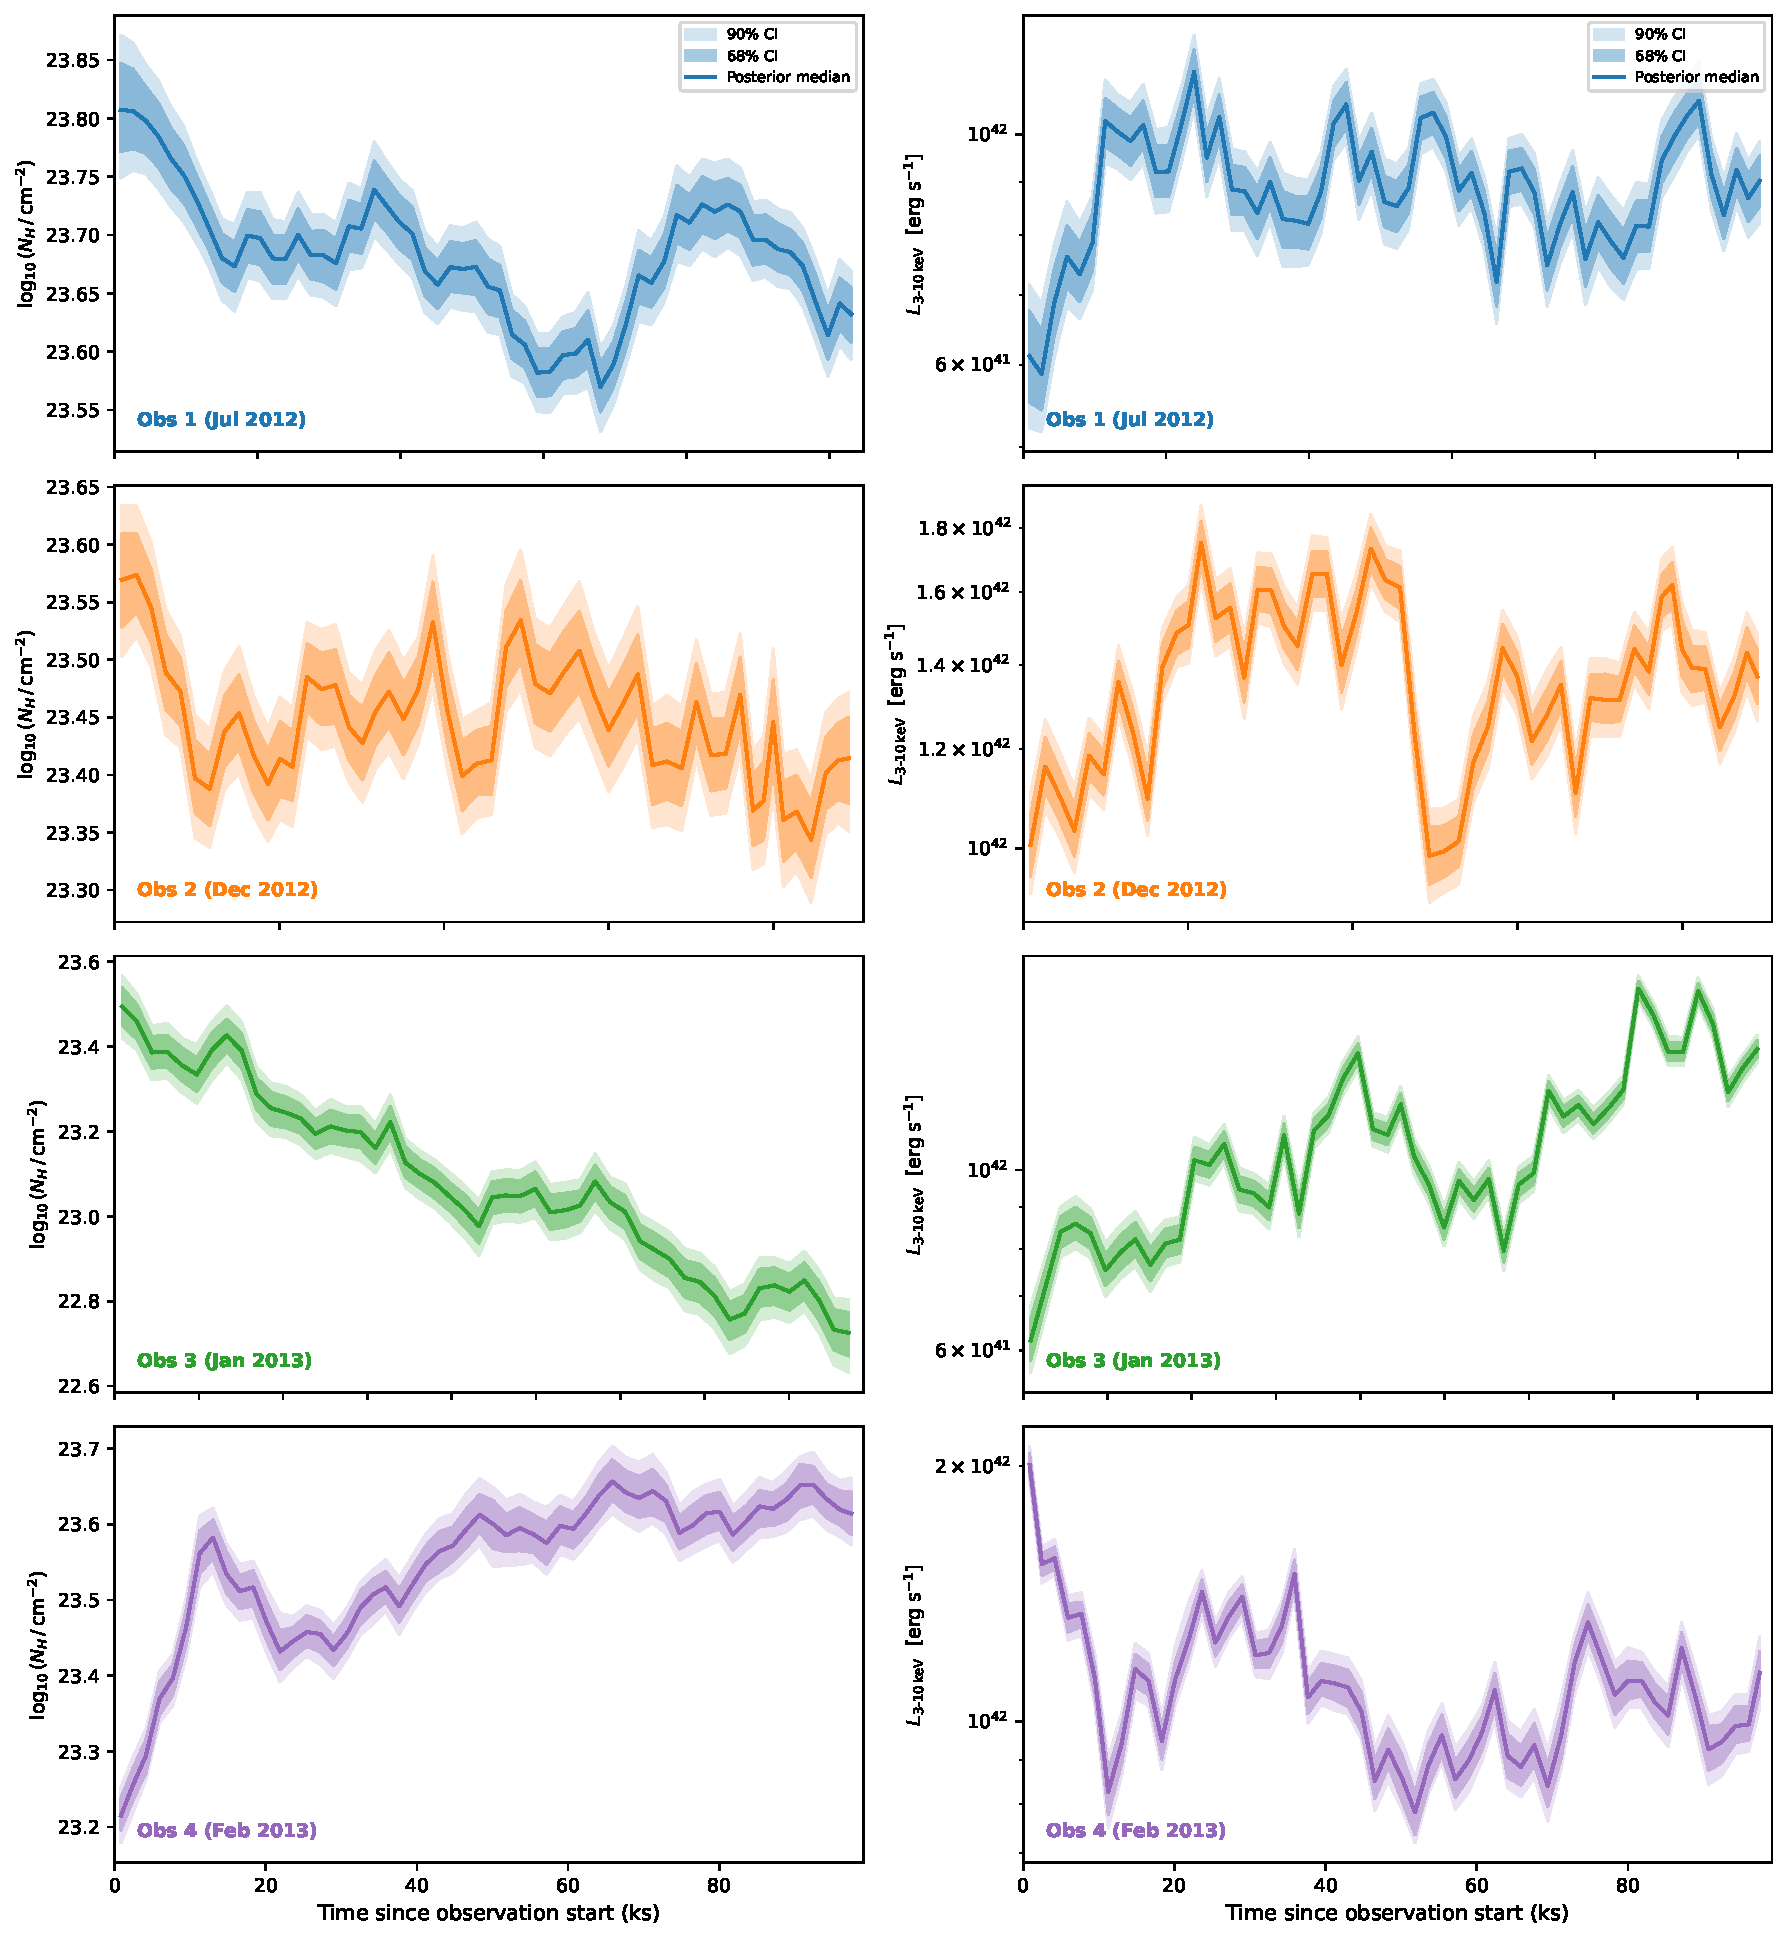
\includegraphics[width=\textwidth]{ngc1365_nh_lum_timeseries.pdf}
  \caption{Posterior time series of the hydrogen column density $\log_{10}(N_H/\mathrm{cm}^{-2})$
  (left column) and the unabsorbed intrinsic 3--10\,keV luminosity $L_{\rm 3\text{-}10\,keV}$
  (right column) for all four NGC\,1365 XMM-Newton observations. Rows correspond to, from top
  to bottom, Obs\,1 (2012 July), Obs\,2 (2012 December), Obs\,3 (2013 January), and Obs\,4
  (2013 February). Solid lines show the posterior median; dark and light shaded bands show the
  68\% and 90\% credible intervals, respectively. The $N_H(t)$ and $K(t)$ processes are inferred jointly by the state-space model,
disentangling absorption-driven spectral variability from intrinsic continuum
variability at each 2\,ks time step. Luminosities are not sampled directly. They are
computed from the posterior normalisation $K(t) = 10^{X_K(t)}$ of the \texttt{zpowerlw}
component, integrated over the rest-frame 3--10\,keV band and converted using a Cepheid
luminosity distance of $d_L = 18.28$\,Mpc \citep{Silbermann1999}, so the credible bands
shown for $L(t)$ propagate from the $K(t)$ posterior. The $x$-axis origin corresponds to
  the start of each observation after good-time-interval filtering.}
  \label{fig:ngc1365_nh_lum_timeseries}
\end{figure*}

\begin{figure*}[ht]
  \centering
  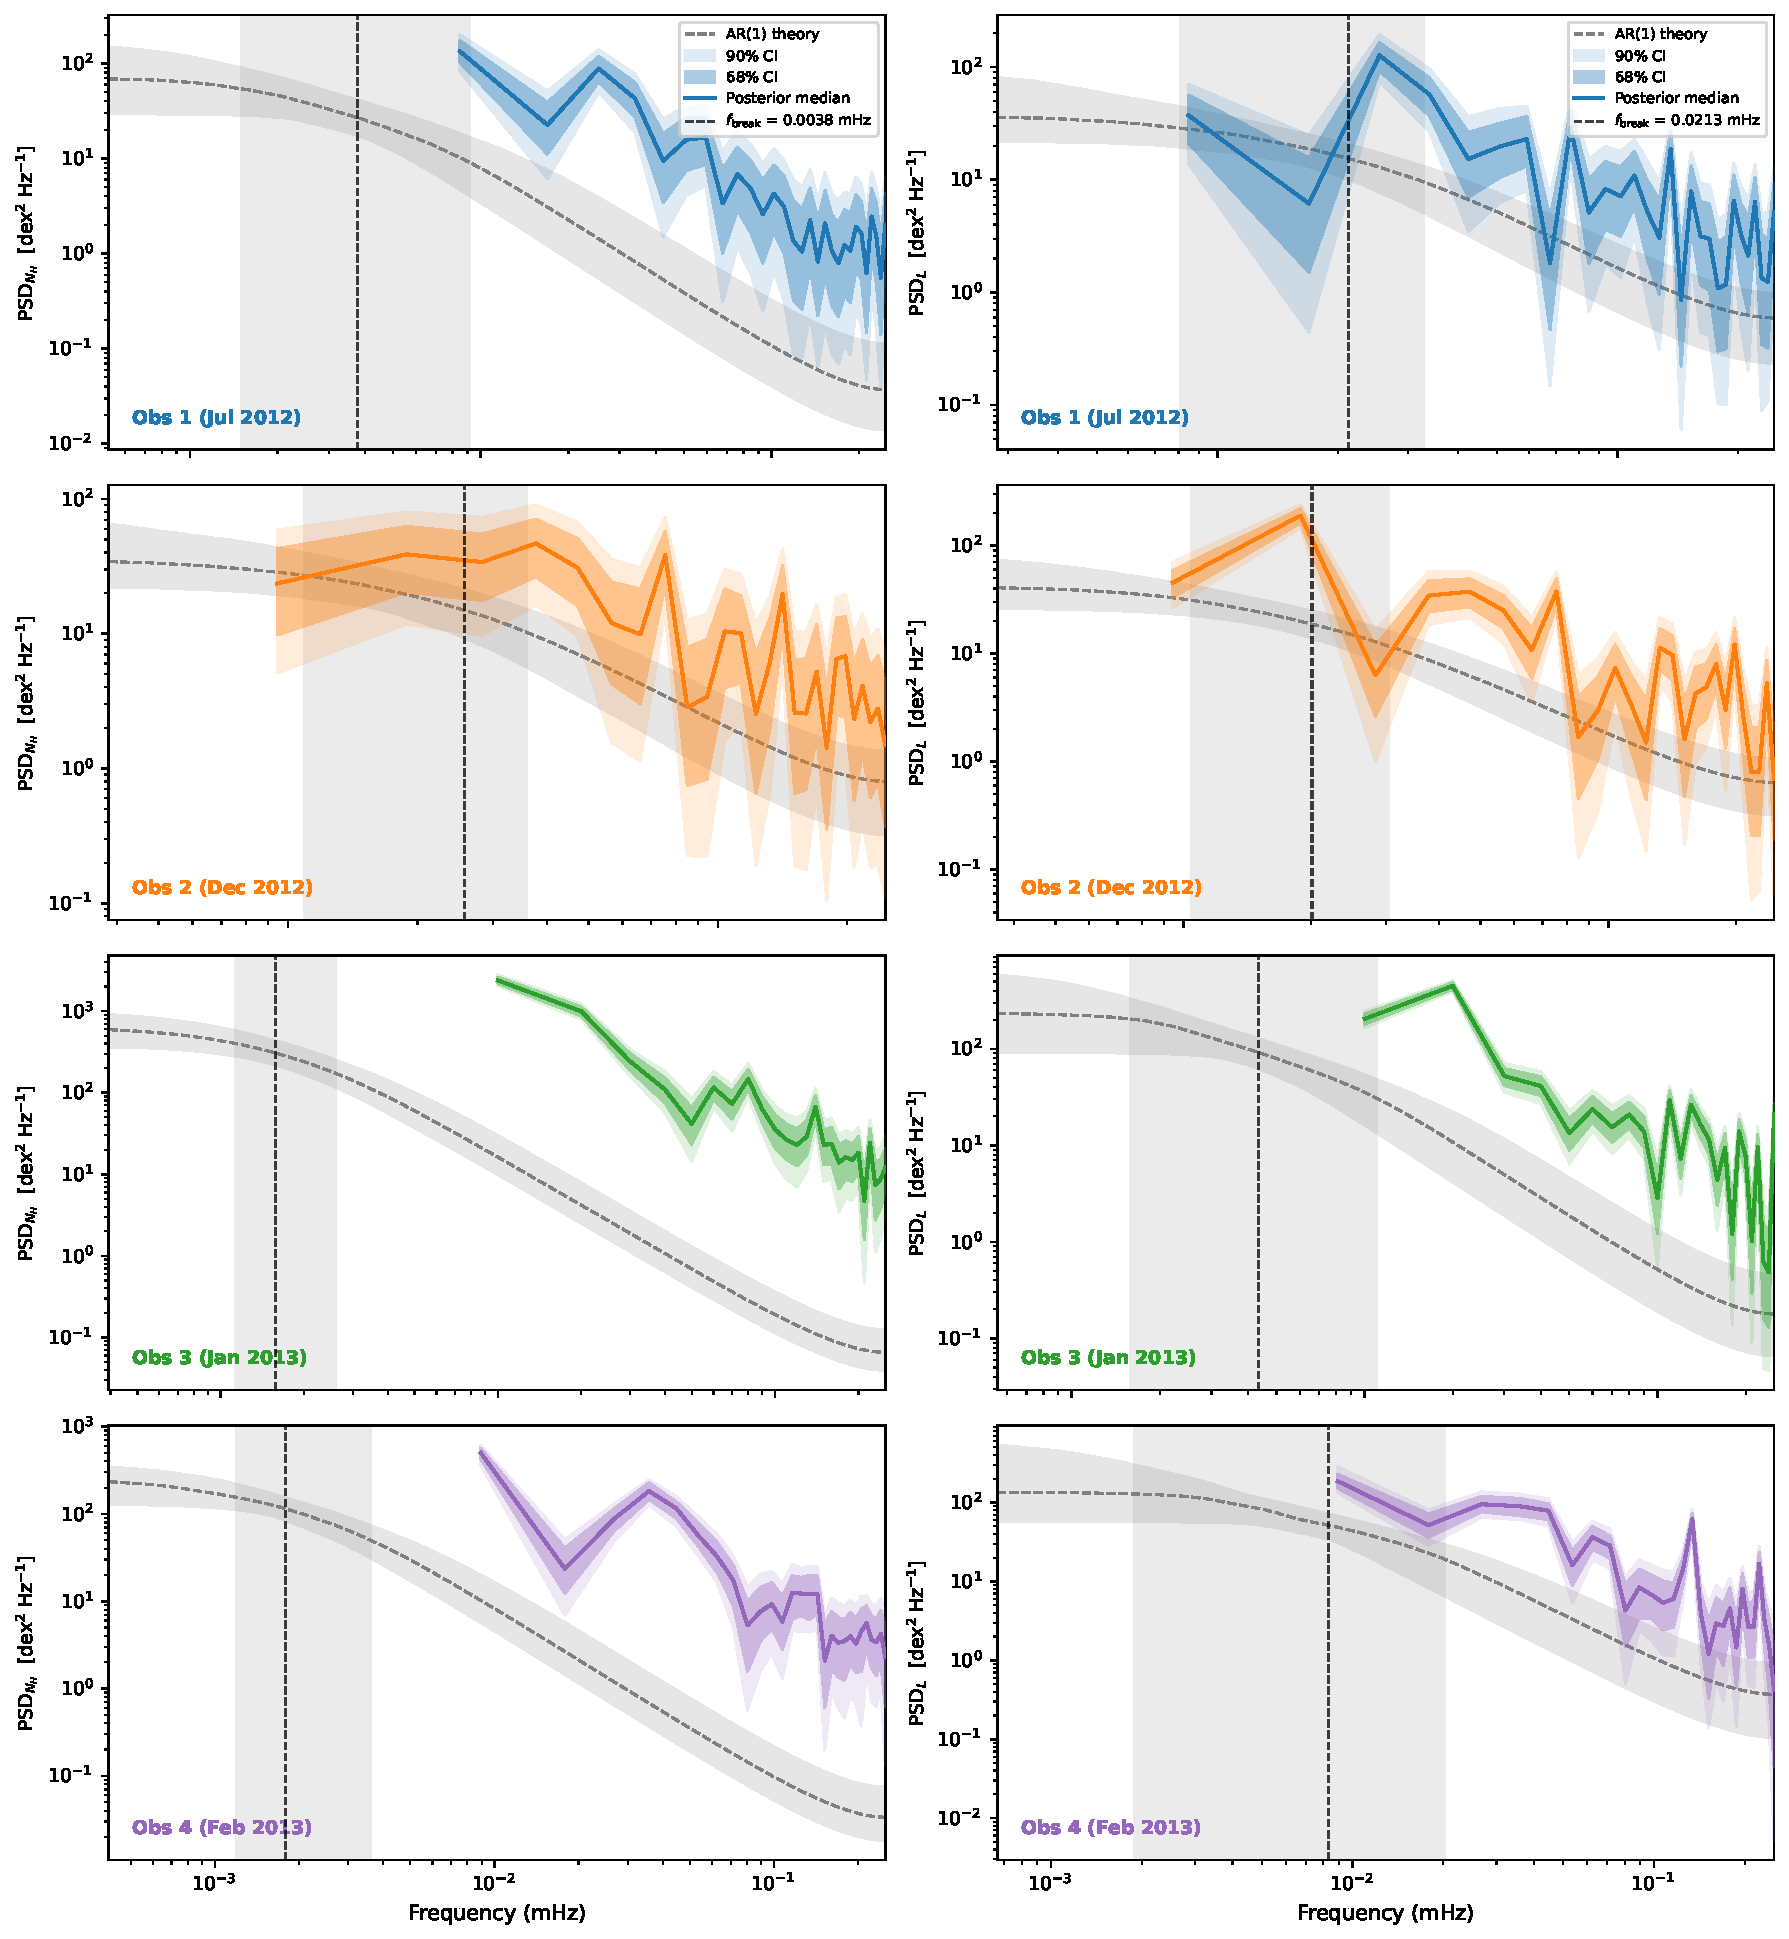
\includegraphics[width=\textwidth]{ngc1365_nh_lum_psd.pdf}
  \caption{Posterior power spectral density (PSD) of $\log_{10}(N_H(t))$ (left column) and
  $\log_{10}(L_{\rm 3\text{-}10\,keV}(t))$ (right column) for all four NGC\,1365 XMM-Newton
  observations (rows as in Fig.\,\ref{fig:ngc1365_nh_lum_timeseries}). Solid coloured lines
  show the posterior median PSD; dark and light shaded bands show the 68\% and 90\% credible
  intervals. The grey dashed line and grey shaded band show the median and 68\% credible interval
  of the theoretical AR(1) PSD, evaluated from the joint posterior samples of $\tau$ and
$\sigma$ with $\phi = \exp(-1/\tau_{\rm bins})$ and $\Delta t = 2\,\mathrm{ks}$. The vertical dashed black
  line marks the posterior median break frequency $f_{\rm break} = (2\pi\tau\,\Delta t)^{-1}$;
  the light grey vertical band shows its 68\% credible interval. At $f \ll f_{\rm break}$ the
  spectrum is flat (white noise); at $f \gg f_{\rm break}$ it falls as red noise. For Obs\,1,
  3, and 4 the posterior median $f_{\rm break}$ of $N_H$ lies below the minimum observable
  frequency $f_{\rm min} = T^{-1}$ set by the observation length, consistent with
  $T < 10\,\tau_{N_H}$; the theoretical AR(1) curve is extended into this unobserved region
  to guide the eye. Any systematic offset between the empirical PSD and the theoretical AR(1) curve is attributable to spectral leakage of power from frequencies below $f_{\rm min}$ into the observed frequency range (see text for details).} % PSD units are dex$^2$\,Hz$^{-1}$.
  \label{fig:ngc1365_nh_lum_psd}
\end{figure*}


\begin{figure}[htbp]
\centering
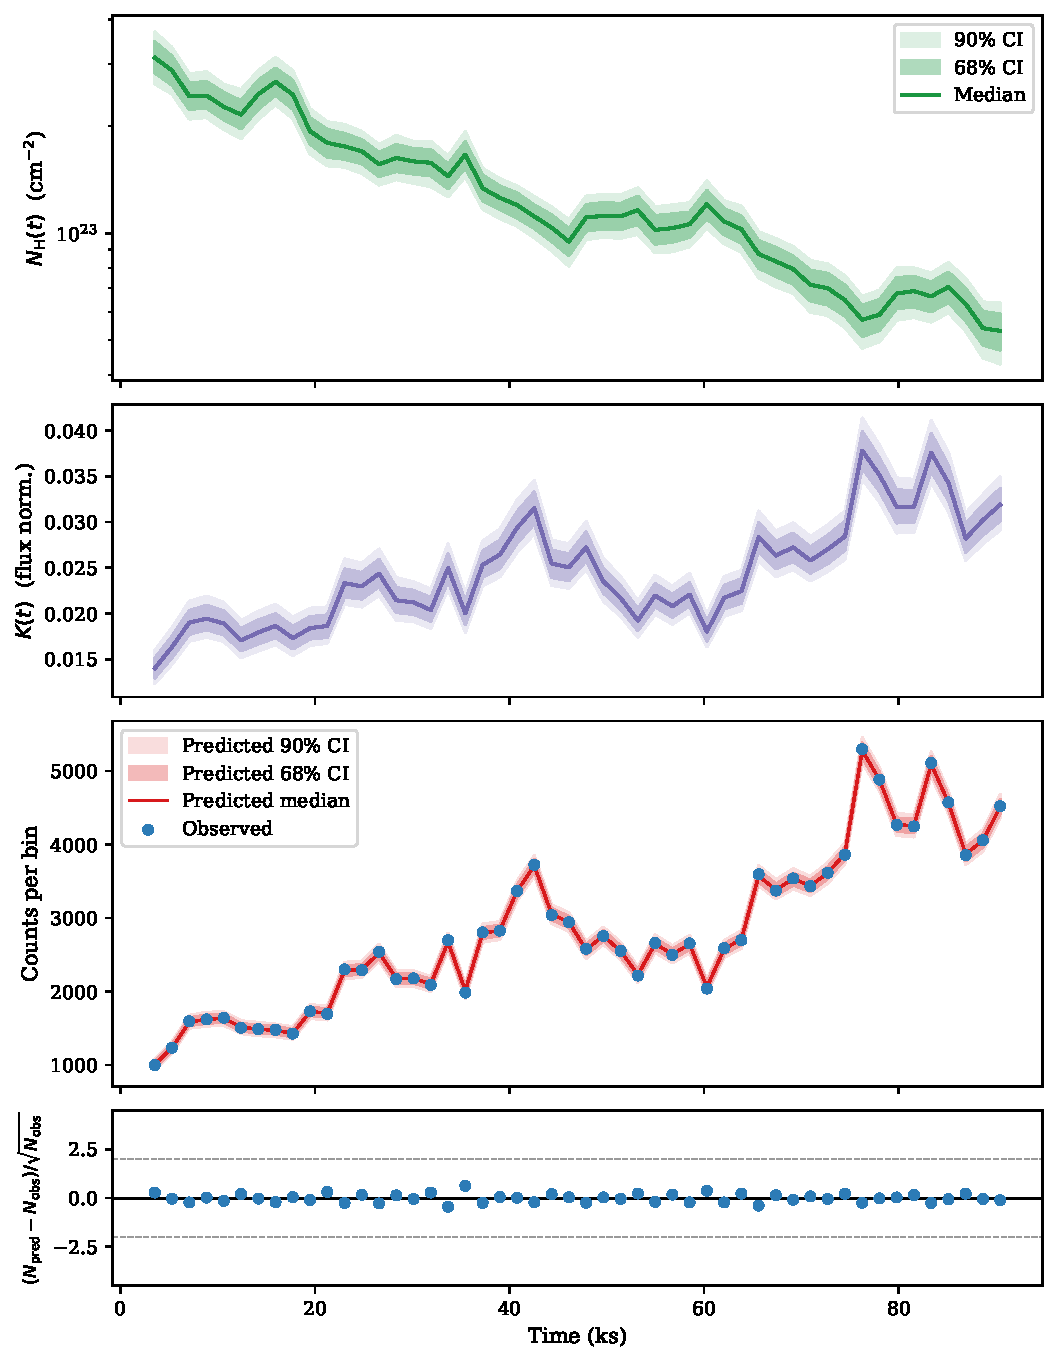
\includegraphics[width=\columnwidth]{ngc1365_obs3_results_4panel.pdf}
\caption{%
Four-panel summary of the HMC inference for Obs\,3 (ObsID\,0692840401,
2013 January 23).
All panels share a common time axis measured from the start of the
observation; each point corresponds to a 2\,ks bin.
\textit{Top:} Posterior time series of the column density
$N_{\rm H}(t)$, showing the median (solid line) with 68\% and 90\%
credible intervals (dark and light shading).
The monotonic decline of $\approx$1\,dex over 85\,ks is consistent
with the absorber uncovering event reported by \citet{Braito2014}.
\textit{Second panel:} Posterior time series of the flux normalisation
$K(t)$, which rises as the absorber retreats.
\textit{Third panel:} Observed counts per bin (blue points) overlaid on
the posterior predictive distribution (median and 90\% credible interval
in red).
\textit{Bottom:} Standardised residuals
$(N_{\rm pred} - N_{\rm obs})/\sqrt{N_{\rm obs}}$,
where $N_{\rm obs}$ is the observed count total per bin and the
denominator is the Poisson standard deviation of the data.
Dashed lines mark the $\pm2\sigma$ level; all bins fall within this
band, with a maximum deviation of $0.6\sigma$.
The inferred photon index is $\Gamma = 2.32$
($90\%$\,CI: $2.28$--$2.37$) and the covering fraction is
$f = 0.91$ ($90\%$\,CI: $0.88$--$0.94$).
}
\label{fig:ngc1365_obs3_4panel}
\end{figure}

Fig. \ref{fig:ngc1365_nh_comparison} shows a comparison between our recovered $N_H$ values and those of several other studies. It is evident that the inferred values follow a very similar pattern as those of other studies across all observations with the caveat that the inferred $N_H$ values are overestimated at observations 1, 2, and 4 but not for observation 3, however, at the cost of higher uncertainties. Given the simplified spectral model we used, this was expected. Our simplified spectral model omits any soft-excess component, and represents neutral reflection through a $pexmon$ component \citep{Nandra2007} of fixed shape ($R = -1$ isotropic reflection, inclination $60^{\circ}$, $\Gamma_{\rm refl} = 2$ matched to the direct power law) whose normalisation is tied to that of the continuum. These parameters are fixed because the Compton hump peaks at $\approx 20$--$30$ keV, outside our $3$--$10$ keV band: without hard-band coverage the reflection strength is essentially unconstrained by the data, and freeing it would compound the $\Gamma$--$N_H$--$f_{\rm cov}$ degeneracy discussed above. Analyses of this source that do constrain reflection self-consistently, such as the \textsc{xillver} modelling of \citet{Rivers2015}, rely on joint XMM-Newton and NuSTAR coverage extending to $\approx 79$ keV, where the Compton hump is directly measurable. The reflected flux is therefore not free to adjust independently of the continuum, and no separate soft component is available at all. This forces our model to generate the remaining observed flux across different energy brackets from the $F_{powerlaw}$ term. This elevates the values of $\Gamma$. On the other hand, $N_H$ and $f_{cov}$ are responsible for the partial absorption of the generated flux within the observed energy intervals. This creates the $\Gamma-N_H-f_{cover}$ degeneracy which makes it hard for the model to break and converge to the true values, especially without NuSTAR energy range coverage. The higher values of $\Gamma$ must be compensated for by the elevated values of $N_H$
and $f_{cov}$. This degeneracy operates within each fit, and is therefore not expected
to produce a correlation between $\Gamma$ and $f_{cov}$ across observations, whose
absorber configurations differ. What the four observations do show consistently is the
effect of absorption on the observed flux. The exposure-corrected count rate (net counts
divided by GTI livetime, Table \ref{tab:ngc1365}) decreases monotonically with
$\mu_{N_H}$ (table \ref{tab:ngc1365_results}), from $1570$ to $514$ counts\,ks$^{-1}$ as
$\mu_{N_H}$ rises from $23.10$ to $23.70$. \\ 
The recovered values of $f_{cov}$ suffer from the degeneracy issue, however, to a lesser extent. $f_{cov}$ for observation 1 and 4 are very close to that of Table 2 of \citet{Braito2014}. On the other hand $f_{cov}$ for observation 3 is significantly overestimated compared to \citet{Braito2014} while it is almost identical with the finding of \citet{Mondal2022} (see their Table 2). Given observation 3 has the lowest photon count, the model tries to suppress the excess photons by increasing $f_{cov}$. It appears in the work of \citet{Braito2014} this suppression is mostly done by $N_H$ as their $N_H$ has higher values than that of \citet{Mondal2022}. This is also apparent in observation 3 of Fig. \ref{fig:ngc1365_nh_comparison} where we can observe the highest variance in the estimated $N_H$ across all the studies. \\
The inferred $\tau$ values show timescales of hours to $\approx$ 1 day, which are consistent with other studies (\citealt{Risaliti2007}, \citealt{Braito2014}). We will discuss the inferred $\tau$ values in more details in Sect. \ref{sec:discussion}. \\
Overall, our framework is able to recover physically meaningful $N_H(t)$ variability for each observation demonstrating convergence across multiple observations with different absorber states. \\

\begin{figure*}[htbp]
    \centering
    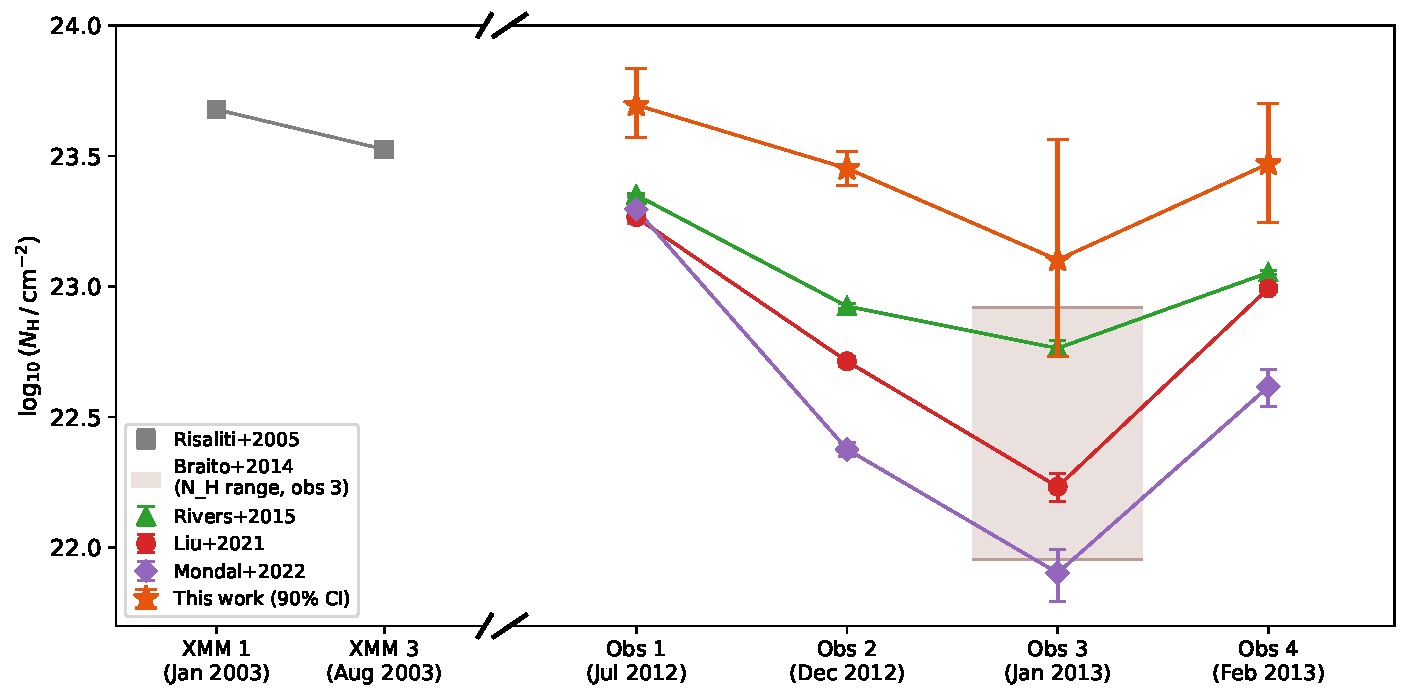
\includegraphics[width=\textwidth]{ngc1365_nh_all_obs_comparison.pdf}
    \caption{%
        Comparison of the time-averaged hydrogen column density $\log_{10}(N_H\,/\,\mathrm{cm}^{-2})$
        for NGC\,1365 across six XMM-Newton observations.
        The left pair of points (XMM\,1 and XMM\,3, January and August 2003) are separated
        from the four 2012--2013 campaign observations by a time break (diagonal marks on the
        horizontal axis).
        Literature values shown are Risaliti et al.\ (2005; grey squares, 2003 observations
        only), Rivers et al.\ (2015; green triangles), Liu et al.\ (2021; red circles),
        Mondal et al.\ (2022; purple circles), and the $N_H$ range reported by
        Braito et al.\ (2014) for Obs\,3 (grey shaded region).
        Orange stars with error bars show the results of this work (90\,\% credible interval
        of the posterior mean $\mu_{N_H}$, i.e.\ the AR(1) long-run mean inferred from the
        HMC posterior).
        Our inferred $N_H$ is elevated relative to the literature for Obs\,1, 2, and 4,
        which we attribute to the simplified spectral model (no soft excess, and
        reflection represented only by a fixed-shape $pexmon$ component with its
        normalisation tied to the direct power law) used in our XMM-only
        3--10\,keV analysis. The limited freedom of these components forces $\Gamma$ to higher values, which in turn requires elevated
        $N_H$ and $f_{\mathrm{cov}}$ to match the observed spectral shape
        (see Sect.~\ref{sec:ngc1365_results}).
        For Obs\,3, our inferred $N_H$ lies within the spread of literature values,
        consistent with the partial-covering absorber being sufficiently optically thick
        during that epoch to constrain $N_H$ more directly from the spectral curvature
        in the 3--10\,keV band.
    }
    \label{fig:ngc1365_nh_comparison}
\end{figure*}


\begin{table}
\caption{Prior distributions for all inferred parameters, NGC\,1365 inference.
         All four observations use identical priors; only the fixed values of
         $N_{H,\mathrm{FC}}$ differ (see footnote).}
\label{tab:ngc1365_priors}
\centering
\begin{tabular}{lll}
\hline\hline
Parameter & Symbol & Prior \\%& Range / scale \\
\hline
\multicolumn{3}{l}{\textit{Scalar parameters}} \\
Photon index       & $\Gamma$            & $\mathcal{U}(1,\,3)$ \\ %& — \\
Covering fraction  & $f$                 & $\mathcal{U}(0,\,1)$       \\  %& — \\
$N_H$ mean (log)   & $\mu_{N_H}$         & $\mathcal{U}(21,\,24)$      \\ %& $\log_{10}(\mathrm{cm}^{-2})$ \\
$K$ mean (log)     & $\mu_{K}$           & $\mathcal{U}(-5,\,0)$       \\ %& $\log_{10}$ (ph\,cm$^{-2}$\,s$^{-1}$\,keV$^{-1}$) \\
$N_H$ timescale    & $\log\tau_{N_H}$    & $\mathcal{U}(\ln 2,\,\ln 80)$ \\%& bins ($\times\,2$\,ks\,bin$^{-1}$) \\
$K$ timescale      & $\log\tau_{K}$      & $\mathcal{U}(\ln 2,\,\ln 80)$ \\%& bins ($\times\,2$\,ks\,bin$^{-1}$) \\
$N_H$ innovation   & $\sigma_{N_H}$      & $\mathrm{HalfNormal}(0.5)$   \\%& dex \\
$K$ innovation     & $\sigma_{K}$        & $\mathrm{HalfNormal}(0.5)$   \\%& dex \\
\hline
\multicolumn{3}{l}{\textit{Fixed (not inferred)}} \\
Full-covering $N_H$ & $N_{H,\mathrm{FC}}$ & fixed$^\dagger$            \\ %& cm$^{-2}$ \\
Galactic $N_H$      & $N_{H,\mathrm{gal}}$ & fixed                      \\%& $1.34\times10^{20}$\,cm$^{-2}$ \\
\hline
\end{tabular}
\tablefoot{%
$\mathcal{U}(a,b)$ a uniform distribution on $[a,b]$;
$\mathrm{HalfNormal}(\sigma)$ the positive half of $\mathcal{N}(0,\sigma)$.
The $\log\tau$ priors are uniform in log-bin space, corresponding to a
log-uniform (Jeffreys) prior on $\tau$, with $\tau \in [2,\,80]$\,bins
$= [0.046,\,1.85]$\,days at the 2\,ks bin spacing.
\\[2pt]
$^\dagger$ $N_{H,\mathrm{FC}}$ fixed at the Rivers et al.\ (2015) Table~2
value for each observation:
$1.0\times10^{22}$\,cm$^{-2}$ (Obs\,1, 4),
$1.4\times10^{22}$\,cm$^{-2}$ (Obs\,2),
$1.1\times10^{22}$\,cm$^{-2}$ (Obs\,3).}
\end{table}


\begin{table*}[ht]
  \centering
  \caption{HMC/NUTS convergence diagnostics for all four NGC\,1365
    observations. $\hat{R}$ is the Gelman--Rubin potential scale
    reduction factor \citep{Gelman1992} in its rank-normalised form;
    values $>1.01$ (bold) indicate potential non-convergence. ESS is
    the bulk effective sample size; values $<200$ (indicated by $\ast$)
    indicate low chain mixing. Both thresholds follow the
    recommendations of \citet{Vehtari2021}.
    Obs~1, 2, and~4 used 3000 warm-up steps and 2000 posterior
    draws; Obs~3 used 5000 warm-up steps and 3000 posterior draws
    to resolve convergence difficulties caused by the soft-wall
    constraint (see Eq.~\ref{eq:hmc_penalisation}).
    All runs used a single chain with \texttt{dense\_mass=True}
    and target acceptance probability of 0.80.
    Parameters shown are the eight global scalar parameters of the
    partial-covering AR(1) model; time-varying trajectories
    $N_{\rm H}(t)$ and $K(t)$ are not shown.}
  \label{tab:hmc_ngc1365_convergence}
  \begin{tabular}{l rr rr rr rr}
    \hline\hline
    Parameter & \multicolumn{2}{c}{Obs 1} & \multicolumn{2}{c}{Obs 2} & \multicolumn{2}{c}{Obs 3} & \multicolumn{2}{c}{Obs 4} \\
    \cmidrule(lr){2-3}\cmidrule(lr){4-5}\cmidrule(lr){6-7}\cmidrule(lr){8-9}
               & $\hat{R}$ & ESS & $\hat{R}$ & ESS & $\hat{R}$ & ESS & $\hat{R}$ & ESS \\
    \hline
    $\Gamma$                  & 0.9995          & 868           & 0.9998 & 2693          & 0.9997 & 3751          & 0.9996 & 1932          \\
    $f_{\rm cov}$             & 0.9995          & 1865          & 0.9995 & 3377          & 1.0021 & 1849          & 0.9997 & 1834          \\
    $\mu_{N_{\rm H}}$         & 1.0031          & 511           & 0.9995 & 515           & 0.9998 & 468           & 1.0024 & 427           \\
    $\ln\tau_{N_{\rm H}}$     & \textbf{1.0206} & 164$^{\ast}$  & 0.9995 & 212           & 1.0074 & 343           & 1.0004 & 171$^{\ast}$  \\
    $\sigma_{N_{\rm H}}$      & \textbf{1.0173} & 197$^{\ast}$  & 1.0016 & 315           & 1.0089 & 333           & 1.0008 & 161$^{\ast}$  \\
    $\mu_K$                   & 1.0020          & 449           & 1.0001 & 1609          & 1.0012 & 828           & 1.0034 & 74$^{\ast}$   \\
    $\ln\tau_K$               & 1.0008          & 124$^{\ast}$  & 1.0003 & 307           & 1.0000 & 228           & 1.0025 & 59$^{\ast}$   \\
    $\sigma_K$                & 1.0005          & 265           & 0.9999 & 441           & 1.0066 & 396           & 1.0024 & 524           \\
    \hline\hline
  \end{tabular}
\end{table*}

\FloatBarrier
\section{Discussion}
\label{sec:discussion}
Earlier we discussed the importance of X-ray variability and how it provides us with the unique opportunity to test our models of the radiation processes and formation and destruction of gas clouds and winds in the vicinity of BHs. In this work we presented a rather different approach to modelling the X-ray variability where we showed we can simultaneously recover the PSD of the observed light curve along with modelling the behaviour of $N_H(t)$ in the form of an AR(1) process over the course of the entire observation while hardness-ratio methods provide only a point estimate of $N_H(t)$ for the entire observation, and time-resolved spectroscopy trades temporal resolution against the counts each segment requires --- \citet{Huang2026}, for instance, require at least 20\,000 net counts per segment, and note that the inferred absorber variations depend on the binning scheme adopted. At the core of our approach is the concept of state-space modelling where $N_H(t)$ and $K(t)$ are treated as latent variables and photon counts as observed dependent variable. The treatment of $N_H(t)$ as an AR(1) provides us with a new tool to shed light on topics such as geometry, location, homogeneity, and structure of the absorbers. Specifically, a unique advantage of our model is that it provides a posterior distribution on the $\tau$ and $\sigma$ parameters of both $N_H(t)$ and $K(t)$ processes. These parameters can be used in interpretation of the variability of the absorber and corona, respectively (see below). \\
Our model, similar to others, comes with its limitations. Through a series of simulations we showed our model, under certain conditions, struggles to convert to the correct $\beta$ index or $\tau$ (see Sect. \ref{sec:limitation}). In the following we use the recovered results of the simulated and NGC 1365 data to discuss the strengths and weaknesses of our framework. \\

\subsection{NGC 1365 as a validation benchmark}
\label{sec:discuss_ngc1365}
We tested the performance of our approach on real world XMM-Newton data of NGC 1365. We chose NGC 1365 as a validation target as it is well-studied and is known for its rapid variability and showing different states of absorber. This object is an ideal target for testing our hypothesis that the partial covering factor can be modelled as an AR(1) process and that we can recover meaningful $N_H(t)$ variability on an object with known literature values. To achieve this we deliberately chose a simplified spectral model and did not use NuSTAR data and limited our analysis to 3 - 10 keV range as our goal was to verify our model and not to run a complete astrophysical study of NGC 1365. \\
Additionally, to compare our inferred results with those of the other studies we converted the inferred $K(t)$ to intrinsic X-ray luminosity. To achieve this we adopted a Cepheid distance of $D = 18.28$ Mpc (\citealt{Silbermann1999}). \\

\subsection{The four observations as distinct absorber regimes: cloud geometry and crossing timescales}
\label{sec:discuss_hmc_diagnostic}
Our model has been able to recover the time variability of $N_H$ across the four observation intervals (Fig. \ref{fig:ngc1365_nh_lum_timeseries}). \citet{Pietrini2019} developed an analytical model of the minimum and maximum projected radius of the X-ray absorbing portion of the eclipsing clouds in the BLR and tested their model on NGC 1365 and several other objects. They define the minimum radius to be $R_1 = 0.4$ $R_X$ where $R_X$ is the radius of the X-ray emitting region. \citet{Pietrini2019} define the upper limit for the radius, $R_2$ and \citet{Pietrini2024} find $R_2/R_X=23.7$ for NGC 1365. Then, following \citet{Torricelli2014}, $R_X \approx 2.5 R_S$ where $R_S$ is given as follows, 
\begin{equation}
\label{eq:schild_radius}
R_S = 2GM_{BH}/c^2.
\end{equation}
Inserting the BH mass of NGC 1365 ($\log(M_{\rm BH}/M_\odot) = 6.65 \pm 0.09$; \citealt{Ricci2017}), $R_S \approx 1.33 \times 10^{12} cm$ and $R_X \approx 3.3 \times 10^{12} cm$ we get $R_2 \approx 7.82 \times 10^{13} cm$. Finally, we estimate the eclipse duration, $t_{ecl}$, as follows, 
\begin{equation}
\label{eq:eclipse_duration}
t_{\rm ecl} = 2(R_{cloud} + R_X)/v_{\rm cloud},
\end{equation}
where we use a factor of 2 as the eclipsing cloud has to sweep its full diameter across the line of sight. Having estimated $R_X$ for NGC 1365 and assuming a cloud velocity of $v_{cloud} = 4000$ km $s^{-1}$ (see \citealt{Torricelli2014}) and replacing $R_{cloud}$ with the maximum and minimum cloud sizes ($R_1$ and $R_2$) the plausible range of eclipse duration for NGC 1365 is $ 0.267 \le t_{\rm ecl} \le 4.7$ days or $ 23 \le t_{\rm ecl} \le 407$ ks. \\
In the context of eclipsing clouds the trajectory of the clouds is of significant importance. \citet{Pietrini2024} defines the "impact parameter", $d$, (see also \citealt{Torricelli2014}) where it measures the distance between the X-ray source centre and the trajectory of the cloud centre projected on the plane of sky. Assuming $\tau_{N_H}$ is approximately identical to the eclipse duration ($t_{\rm ecl} = \tau_{N_H}$) during each observation, and the clouds are spherical and d = 0, then for observations 1, 3, and 4, all $\tau_{N_H}$ values fall within the plausible range; observation 2 is the exception and is discussed separately (see Table \ref{tab:ngc1365_results}). For the rest of this discussion we assume these assumptions hold. \\
Given $t_{\rm ecl}$ has been inferred for different observations, the next question would naturally be whether our inferred $\tau_{N_H}$ values would yield a reasonable eclipsing cloud size. To answer this question we use Eq. \ref{eq:eclipse_duration} once again, with the same set of assumptions on the geometry and trajectory of the clouds, except this time we use $\tau_{N_H}$ as the eclipse duration and we solve for $R_{cloud}$ (see Table \ref{tab:cloud_properties}). \\
With maximum and minimum eclipse durations estimated along with the size of the eclipsing clouds we will discuss the validity and credibility of our inferred values for each observation in more detail. \\ 

\subsubsection*{Observation 1}
The estimated $\tau_{N_H}$ for observation 1 is $0.49$ days or $\approx 42$ ks. This is well within the allowed maximum and minimum values of $N_H$ variations estimated by \citet{Pietrini2024}. However, there is no explicit estimation for the duration of the eclipsing clouds in observation 1 in the literature so a direct comparison is not feasible. In addition, our estimated covering factor in observation 1 is $0.97$ which is very close to the full covering factor 1 found by \citet{Rivers2015} for observation 1. \\
Looking at Fig. \ref{fig:ngc1365_nh_lum_timeseries} an interesting feature of the recovered $N_H$ time series for observation 1 is the bump at $\approx 80$ ks. Given its symmetrical profile and its duration which is $\approx 40$ ks (with the rest of the increase out of the frame) it seems reasonable to interpret this pattern as an eclipsing cloud passing across the line of sight. This pattern is also visible in the work of \citet{Rivers2015}, however, to a lesser extent as they only have four data points (see Fig. 3 of their work). It is worth mentioning that there is another feature that appears to be a second bump visible at the very beginning of the same $N_H$ curve, however, the left side of this bump is not visible which makes it hard to interpret this feature as another eclipsing event. \\
Looking at Fig. \ref{fig:ngc1365_nh_lum_timeseries} the intrinsic luminosity of observation 1 shows a significant increase in the first 10 ks of the observation whereas the rest of the observation it shows a stable behaviour with no significant increase or decrease. This seems to be in agreement with the finding of \citet{Rivers2015}, however, their power-law flux curve is comprised of only four data points which makes it hard for a direct comparison (see their Fig. 3). \\
Finally, the estimated cloud size for this observation falls within the acceptable range of cloud size estimated for NGC 1365. \\

\subsubsection*{Observation 2}
Our estimated $\tau_{N_H} = 0.072$ days for observation 2 is a factor of four smaller than the minimum possible eclipse duration, 0.267 days, estimated according to the method of \citet{Pietrini2024}. This might seem like a wrong estimate, however, we argue that this is not a mistake and in fact it is the capability of our model in recovering eclipse durations as short as $\approx 100 $ minutes. This apparent contradiction originates from the fact that the method of \citet{Pietrini2024} is based on the analysis of the statistically significant HR variations while our method has the advantage that it uses the recovered $N_H$ curve directly to estimate the eclipse duration. \citet{Pietrini2024} state that their method is sensitive to occultations with durations between $\approx 10$ ks and $\approx 1$ day (see \citet{Torricelli2014} for a detailed discussion of the HR-based method). Thus, we argue that our method is capable of detecting eclipses that are shorter than the minimum duration suggested by HR-based method of \citet{Pietrini2024} and \citet{Torricelli2014}. \\
Looking at Table \ref{tab:cloud_properties}, we can see there is no cloud size for observation 2. The reason is that inserting the values of $\tau_{N_H}$ for this observation along with clouds velocity yields a negative value for cloud size, which is unphysical. This negative value is the result of our set of assumptions above that the cloud is spherical and $d = 0$. If we relax our assumption on $d$ and allow for non-central transit we can solve for $d$ using equation 2 of \citet{Pietrini2024} with the assumption that $f_{abs} = R_1/R_X = 0.4$ which is the minimum cloud size for NGC 1365 and one reaches $d = 1.348 R_X$. Given that for an eclipse to occur at all, there must be an overlap between the source and the eclipsing cloud on the plane of sky which requires $d < 1 + f_{abs}$ (the condition for two circles $R_X$ and $R_{cloud}$ to overlap). Our $d = 1.348$ passes this condition by a very small margin of $0.052$ which means the eclipsing cloud of size $0.4R_X$ is grazing the source on the plane of sky. Interestingly, larger clouds can reproduce the same $\tau_{N_H} = 6.2$ ks at correspondingly larger impact parameters, always with a small but nonzero covering fraction. \\
Similar to observation 1 the power-law flux of the observation 2 in \citet{Rivers2015} is only based on four data points. Thus, a direct comparison is hard, however, we can see our estimated intrinsic luminosity during observation 2 matches well with that of the Rivers et al. This is especially visible in the third data point of their plot which shows a sudden dip around 50 ks which is clearly captured in our estimated luminosity plot (see Fig. \ref{fig:ngc1365_nh_lum_timeseries} and Fig. 3 of \citealt{Rivers2015}). \\

\subsubsection*{Observation 3}
The estimated $\tau_{N_H}$ for observation 3 is $\approx 1.174$ days or $\approx 100$ ks. This is in very good agreement with the finding of \citet{Braito2014} where they find a decrease in $N_H$ from $10^{23}$ $cm^{-2}$ to $10^{22}$ $cm^{-2}$ in a 100 ks timescale during observation 3. \\
Assuming a central transit and a spherical shape we estimate the eclipsing cloud radius to be $1.69 \times 10^{13} cm  = 5.12 R_x$. The estimated cloud radius of $5.12 R_X$ falls within the acceptable range $[R_1, R_2] = [0.4, 23.7] R_X$ for NGC 1365. Our estimated $1.69 \times 10^{13}$ cm implies a diameter of $3.38 \times 10^{13}$ cm, in excellent agreement with the $\Delta R \approx 3 \times 10^{13}$ cm estimated by \citet{Braito2014}. Note, however, that they adopt a cloud velocity of $3000$ km s$^{-1}$ whereas we assume $4000$ km s$^{-1}$ following \citet{Torricelli2014}. Rescaling their estimate to $4000$ km s$^{-1}$ gives $\Delta R \sim 4 \times 10^{13}$ cm, and our inferred diameter of $\approx 3.4 \times 10^{13}$ cm remains consistent within this uncertainty. \\
\citet{Rivers2015} find that in observation 3 the covering factor and $N_H$ both decline and state that this behaviour is unusual. They use this finding to suggest a wind from the accretion disc or an opening in the BLR or torus clouds as possible explanations for the origin of the obscuring material in observation 3. The simultaneous decline in $N_H$ and covering factor is also apparent in our inferred values as observation 3 has the second lowest inferred covering factor ($f_{\rm cov} = 0.908$), however, the origin of the absorber in observation 3 is beyond the scope of this work (see \citealt{Braito2014} and \citealt{Rivers2015} for a detailed discussion of observation 3). \\
Our inferred luminosity of observation 3 resembles the curve estimated by \citet{Rivers2015} closely (see their Fig. 4). It starts at the lowest values and rises slowly in the beginning of the observation while it plateaus in the middle of the observation and it rises again towards the end of the observation. Fig. \ref{fig:ngc1365_obs3_4panel} shows the $K(t)$ curve for observation 3 and how the photon count curve closely follows the $K(t)$ along with $N_H(t)$. \\

\subsubsection*{Observation 4}
Observation 4 is the last observation interval with an estimated $\tau_{N_H}$ of $1.028$ days or $\approx 89$ ks. Unfortunately, a direct comparison of our inferred $\tau_{N_H}$ is not viable as there is no estimated value in the literature for this observation interval. Using the estimated values of \citet{Rivers2015} for observation 4 and using a range of BH mass, BLR radius, and cloud velocities, we get a wide range of estimates for $\tau_{N_H}$ from $\approx 91$ ks which is in excellent agreement with our estimate to $\approx 36$ ks which is a factor of $\approx 2.4$ smaller. \\
Looking at the inferred $N_H$ curve for observation 4 and that of the \citet{Rivers2015} (see their Fig. 3 and 7) we see a good agreement between the two curves, however, there is a difference between the location of the peak in the first 32 ks of the curves. In our inferred curve the $N_H$ peak happens at around $\approx 10$ ks whereas in Rivers et al. happens at around $\approx 25$ ks. This difference is possibly due to the different methodologies used in our work and their work as our method uses a joint inference of $N_H(t)$ and $K(t)$ without freezing parameters while \citet{Rivers2015} freeze several model parameters (reflection, full-covering absorber) and use 4 ks sub-intervals over only the first 32 ks. \\
It is important to note that our model captures the temporal structure of $N_H$ beyond 32 ks and we can see $N_H$ continues to rise and it has its second and highest peak at around $64$ ks. However, this peak is not captured in \citet{Rivers2015} due to the resulting fewer data points from each interval analysis. The ability of our model in capturing temporal structure of $N_H$ beyond 32 ks is possibly the reason behind the difference between our $\tau_{N_H}$ and the eclipse duration implied by the \citet{Rivers2015} analysis. \\
Furthermore, \citet{Rivers2015} show that the covering factor in observation 4 remains stable and on average close to $0.95$ throughout the entire observation. This is also in excellent agreement with our estimated value of covering factor (see Table \ref{tab:ngc1365_results}). \\
Finally, using our inferred $\tau_{N_H}$ of observation 4 we estimate the size of the eclipsing cloud to be $\approx 1.44 \times 10^{13} cm  = 4.36 R_x$. Our estimated cloud size is larger than $\approx 4 \times 10^{12} cm$ estimated by \citet{Rivers2015} by a factor of $\approx 3.6$. Different cloud velocity, BH mass, and BLR radius for cloud size estimation is the main driver of this difference. In addition, \citet{Rivers2015} only use the first $32$ ks of the observation to estimate the clouds size whereas our estimate of cloud size is the result of applying the inferred $\tau_{N_H}$ of observation 4 based on the entire recovered $N_H$ curve including and beyond the first $32$ ks. \\
\citet{Rivers2015} estimated the flux for the first 32 ks of the observation 4 (see their Fig. 7) which matches well with the first 32 ks of our inferred luminosity (see Fig. \ref{fig:ngc1365_nh_lum_timeseries}). Luminosity starts highest and drops and then rises again, however, not to the highest levels where it started. From 32 ks onward our derived luminosity shows a relatively stable behaviour with no specific trend which seems to match the finding of \citet{Rivers2015} in their Fig. 3, however, their resolution is very coarse. \\

\begin{table*}[ht]
  \centering
  \caption{Cloud properties derived from the posterior decorrelation
    timescale $\tau_{N_H}$ for each NGC\,1365 observation, assuming
    a cloud velocity $v_{\rm cloud} = 4000$\,km\,s$^{-1}$ and
    $R_X = 3.3\times10^{12}$\,cm. The cloud radius is estimated from
    the central-transit formula $R_{\rm cloud} = v_{\rm cloud}\,
    \tau_{N_H}/2 - R_X$.}
  \label{tab:cloud_properties}
  \begin{tabular}{lcccc}
    \hline\hline
    Obs & Date &  $f_{\rm cov}$ & $\tau_{N_H}$\,(ks) &
      $R_{\rm cloud}$\,(cm) \\
    \hline
    1 & 2012-07-25 & 0.974 & 42.3  & $5.17\times10^{12}$\,$\approx 1.57\,R_X$ \\
    2 & 2012-12-24 & 0.856 &  6.2  & $\dagger$ \\
    3 & 2013-01-23 & 0.908 & 101.4 & $1.70\times10^{13}$\,$\approx 5.15\,R_X$ \\
    4 & 2013-02-12 & 0.949 &  88.8 & $1.45\times10^{13}$\,$\approx 4.38\,R_X$ \\
    \hline\hline
  \end{tabular}
  \tablefoot{%
    $\dagger$ Obs\,2 yields an unphysical negative $R_{\rm cloud}$
    under the central-transit assumption ($f_d = 0$), because
    $\tau_{N_H} = 6.2$\,ks is shorter than the minimum possible
    central-transit duration $2R_X/v_{\rm cloud} = 16.5$\,ks.
    This is consistent with a near-grazing geometry
    ($f_d \approx 1.35\,R_X$, margin $0.05\,R_X$ from a complete miss)
    of a minimum-size cloud ($R_{\rm cloud} \sim 0.4\,R_X
    \approx 1.3\times10^{12}$\,cm).
  }
\end{table*}


\subsection{Towards a complete analysis: what the next step looks like}
\label{sec:discuss_future_work}
In this study we developed a methodology to estimate $\beta$ index of the PSD of the observed photon curve while, simultaneously, recovering $N_H(t)$ and $K(t)$ which in turn enabled us to estimate the eclipse duration. A natural question to ask would be whether there are any connections between the eclipse duration and the mass of the central BH. The establishment of an empirical correlation between $M_{BH}$ and the large-scale properties of its host galaxy is known as "scaling relation". The scaling relations are of particular interest because they provide a framework for the co-evolution of the central BH and its host galaxy. This has prompted a variety of studies in establishing scaling relations between the soft and hard X-ray time lags and $M_{BH}$ (\citealt{Mallick2021}) to different accretion disc timescales and $M_{BH}$ (\citealt{Kelly2009}) to bend frequency of PSD and $M_{BH}$ (\citealt{GonzalezMartinVaughan2012}). Notably, \citet{Kelly2009} made an attempt to model the UV/optical variability of quasars using a DRW model of the form CAR(1). After estimating $\tau$, for a series of quasars they establish a relationship between the estimated $\tau$ values and $M_{BH}$ of the quasars in their sample. Therefore, within the framework of eclipsing clouds in AGNs and XRBs, a natural extension of our work would be to investigate the plausibility of establishing a scaling relation between $\tau_{N_H}$ and $M_{BH}$. \\
To accomplish such an undertaking one has to collect a statistically meaningful sample of variable AGNs/XRBs. While this requirement alone may not be hard to achieve, given what we discussed in Sect. \ref{sec:limitation}, the length of the light curve for such variable objects must meet $T \ge 10\tau$ which would significantly reduce the number of objects that would meet both the sample size and long observation criteria. However, as we discussed earlier, $T \ge 10\tau$ may not be a hard requirement, especially if the observed energy channels of the collected objects cover the energy range that goes beyond $\approx 50$ keV. In other words, one may be able to justify the use of objects with $ T < 10\tau$ if there is a good energy range coverage for those objects. The higher energy range coverage breaks the $\Gamma$–$f_{\rm cov}$–$N_H$ degeneracy which in turn tightens the posterior on $N_H$ at each time step, effectively increasing the information content per observation interval. \\


\subsection{Model limitation}
\label{sec:limitation}
\subsubsection{The case for $\tau$}
Earlier, in Sect. \ref{sec:verification_results}, we presented the results on the recovery of different combinations of parameters of interest. We noted for observations with a length of $T<10\tau$ the true $\tau$ could not be constrained well (see Table \ref{tab:light_curve_sim_table}). In other words, the larger the difference between $T$ and $\tau$ the wider the confidence interval on the recovered $\tau$. This behaviour is already known and is discussed in detail in \citet{Kozlowski2017}. \citet{Kozlowski2017} finds that the minimum length of observation required, $T$, to constrain the decorrelation timescale, $\tau$, is $T \ge 10 \tau$ and for observation where this condition is not met the inferred $\tau$, will fall in the so-called "unconstrained" region. \citet{Kozlowski2017} argue that the inferred decorrelation timescales that fall in this region will have a distribution with a median equal to $20\% - 30\%$ of the length of the observation regardless of the true underlying decorrelation timescale. \citet{Kozlowski2017} states that the main issue is that for processes where PSD $\propto \nu^{-\beta}$ if $T < 10 \tau$ the flat part of the PSD is not explored, which in turn leads to an inaccurate estimate of $\tau$. \\
Looking at our results we observe that the length of observations 1, 3, and 4 are significantly lower than the $10\tau$ threshold while observation 2 passes the threshold criterion. Looking at Fig. \ref{fig:ngc1365_nh_lum_psd} we also see that none of the estimated PSD of $N_H$ and intrinsic luminosity extends to the flat part of the spectrum. Only in observation 2 there is a slight coverage of the flat part of the spectrum. Also, there is a clear constant off set between the estimated PSD and the median PSD along with the flattening of the PSD towards higher frequencies which signify power leakage (see Sect. \ref{sec:psd_BH_properties}). This may imply that our results are not valid, however, we argue against it with the following reasons. \\
First, we point out that of the three observations with $T < 10\tau$ none of them has a $\tau$ that is $20\% - 30\%$ of the length of the observation: the recovered values correspond to $36\%$, $101\%$ and $78\%$ of $T$ for observations 1, 3 and 4 respectively. This is in direct contrast with the finding of \citet{Kozlowski2017}. The comparison is sharpened by asking where a prior-dominated posterior would fall. Our prior on $\log \tau_{N_H}$ is uniform on $[\ln 2, \ln 80]$ bins, with geometric mean $12.6$ bins, or $21\% - 25\%$ of $T$ for these three observations. The ``unconstrained'' value reported by \citet{Kozlowski2017} is therefore close to what our prior alone would return, and our posteriors sit well above it, indicating that the data do inform $\tau_{N_H}$ rather than the prior determining it. Second, the $T \ge 10 \tau$ threshold proposed by \citet{Kozlowski2017} is the result of DRW model applied to photometric data whereas we use spectroscopic data and both $N_H(t)$ and $K(t)$ are constrained by the photon counts across multiple energy channels. In other words, our spectroscopic data carry more information than photometric data which in turns allows us to constrain the parameters of the model even more. Extending our analysis to higher energy channels, covered by NuSTAR, would likely allow us to constrain $\tau$ even better by breaking the $\Gamma-f_{cov}-N_H$ degeneracy. Third, $T \ge 10 \tau$ is not a hard criterion. This means failing to meet this criterion does not mean failure in estimating the true value of $\tau$. It simply means the confidence interval on $\tau$ would be wider which in turn means a less accurate, and not necessarily wrong, estimate of $\tau$. Finally, our strongest argument in support of our inferred $\tau$ values is the confirmation we achieved by comparing our results with those of other studies despite other studies using different methodologies (see Sect. \ref{sec:discuss_hmc_diagnostic}), quantified below for observation 3. \\
This does not mean $\tau_{N_H}$ is fully determined in every observation. The posteriors are truncated by the prior at both ends. For observations 3 and 4, $42\%$ and $34\%$ of the posterior mass lies in the upper tenth of the prior range, with $95$th percentiles reaching $97\%$ and $95\%$ of the ceiling at $\tau_{\rm max} = 1.85$ d; these values are therefore lower bounds rather than two-sided measurements, and the cloud sizes derived from them in Table~\ref{tab:cloud_properties} inherit that status. Observation 2 shows the opposite behaviour, with $45\%$ of its mass in the lowest tenth of the prior range and a fifth percentile at the floor $\tau_{\rm min} = 0.046$ d, making it an upper bound. Only observation 1, with $14\%$ of its mass near the ceiling, is bounded on both sides within the prior range. \\
That the posteriors are truncated does not imply they are prior-determined. For observation 3, the recovered $\tau_{N_H} = 1.174$ d agrees to within $1.4\%$ with the $\approx 100$ ks decline timescale reported independently by \citet{Braito2014}, and lies a factor of four above the geometric mean of the prior. A posterior determined by its prior would carry no such external agreement. \\
Overall, our methodology is capable of recovering $N_H(t)$ and $K(t)$ that are in good agreement with the findings of other studies. Furthermore, our model needs to be tested on a more diverse set of objects such as XRBs and AGNs and at different redshifts for further verification of its performance. \\
We note one respect in which our parameterisation avoids a known caveat of OU-based models. \citet{Kankkunen2025} point out that an OU/DRW process has a Gaussian PDF, whereas the PDFs of AGN light curves cannot be purely Gaussian since they admit no negative values. Because we place the AR(1) process on $\log N_H$ and $\log K$ rather than on the fluxes themselves, the implied distributions are log-normal and strictly positive by construction. \\

\subsubsection{The case for $\beta$}
In Sect. \ref{sec:verification_results} we showed that a larger duration of the observation, $T$, compared to the decorrelation timescale, $\tau$, will result in a higher number of bins falling on $ f < f_{bend}$, which in turn produces a flatter estimation of $\beta$ and, consequently, a misrepresentation of the actual value of the underlying $\beta$ (see Fig. \ref{fig:psd_beta_recovery_tau2} and \ref{fig:psd_beta_recovery_tau2_t500}). It is important to note that this is not a modelling issue rather this behaviour is the result of finite observation of long term processes with PSD $\propto f^{-\beta}$. Regardless, this shows our model is not immune to this fundamental property of long memory process and it gives us a sense of the timescales over which the model fails to recover $\beta$ confidently. \\
Given we have already generated a sample of posterior predictive distribution of $N_H$ and $K$, and the fact that we do not know the true value of $\beta$ for these two processes, estimating $\beta$ for these curves is of low interest. However, as we discussed above and looking at Fig. \ref{fig:ngc1365_nh_lum_psd}, one can see for observations 1, 3, and 4, where $T < 10\tau_{N_H}$, it is very likely the estimation of $\beta$ will yield values that are closer to the true value, whereas in observation 2, where $T \gg \tau_{N_H}$, the estimation of $\beta$ will likely result in flatter values. \\
A related, more extreme illustration of this effect is given by the \texttt{colorednoise} validation in Appendix \ref{app:recovery}. That test infers $\beta$ from a single, aggregate photon-count channel with no energy resolution and no spectral model to exploit, making it the least informative setting used anywhere in this work. Investigating this in detail, we find not one but \emph{two distinct failure modes}, depending on the true $\beta$, rather than a single uniform limitation. \\
For $\beta \lesssim 2$ (illustrated by $\beta = 1.7$), the posterior on $\tau$ is not pinned at either edge of its prior, and once the chain is run long enough to reach an adequate effective sample size it is well converged ($\hat{R} \approx 1$). The true $\beta$ nonetheless falls outside the recovered [5\%--95\%] credible interval (Table~\ref{tab:appendix_params}). This is not a bias in the recovered value, but a mismatch between two quantities that measure different things. The credible interval is the spread of $\beta$ across posterior draws \emph{within a single realisation}, which for $\beta_1$ spans only $1.587$--$1.595$; the scatter \emph{between} independent realisations of the same process is $\approx 0.17$ (Table~\ref{tab:beta_N40_ensemble}), some twenty times larger. The interval is therefore far too narrow to contain the true value, even though the estimator itself is unbiased. An independent test using 40 freshly generated realisations at $\beta = 1.7$ (see Appendix \ref{app:recovery}) shows a genuine realisation-to-realisation spread of comparable size, present even when fitting the generated \texttt{colorednoise} flux itself, rather than the AR(1) reconstruction of it. This is independently confirmed by repeating the full inference pipeline (real Poisson counts through AR(1)/HMC inference and periodogram fitting on the resulting reconstruction, rather than the raw input flux) across 40 realisations, which recovers a mean $\beta$ of 1.67 and a median of 1.68 (true value 1.70), with a realisation-to-realisation standard deviation of $\approx 0.17$ and no statistically significant bias. The limitation therefore comes from uncertainty quantification rather than recovery, and it is a property of estimating a power-law index from a single finite periodogram, not of the AR(1) model or its Bayesian inference; it should persist regardless of the observation's signal-to-noise ratio, and can only be addressed by averaging over multiple independent realisations, since the variance of the periodogram does not decrease as the number of data points increases \citep[][and references therein]{Kankkunen2025}. \\
For $\beta > 2$ (illustrated by $\beta = 3$ and $\beta = 4$), the posterior on $\tau$ instead sits pinned against the upper edge of its prior. The effective sample size is large and $\hat{R} \approx 1$, so this is a well-converged result rather than a sampling artefact. The behaviour reflects a structural property of the AR(1) process. Its power spectrum cannot exceed an asymptotic slope of 2 for any value of $\tau$, because the damped random walk admits only a bend frequency and a normalisation as free parameters and its PSD is therefore a Lorentzian \citep{Kankkunen2025}. A genuinely steeper input consequently forces the fit towards the longest correlation time its prior allows, in an attempt to weaken the model's own mean-reverting structure as far as possible. The mismatch is compounded by the fact that a pure power law is scale-free. Such a process has no bend frequency, and therefore offers no characteristic timescale for $\tau$ to converge on. \\
We tested this directly by repeating the $\beta = 3$ and $\beta = 4$ validation across a range of signal-to-noise ratios (Appendix \ref{app:recovery}). Rather than relaxing the constraint, higher signal-to-noise made the pinning more pronounced, with the posterior mean of $\tau$ moving measurably closer to the prior's upper edge as the count rate increased. This is the opposite of what an information deficit would produce, and it supports the structural explanation above. Additional signal only sharpens the model's confidence that an arbitrarily long $\tau$ is required, pushing the Lorentzian bend further outside the observed frequency range. Widening $\tau$'s prior upper bound from 80 to 500 does not resolve the pinning. The posterior simply moves to a new value near the widened edge ($\approx 460$--$470$), with no meaningful change in the recovered $\beta$. The pinning is therefore a property of the model-data mismatch rather than an artefact of the particular bound chosen. \\
A further limitation concerns the assumption of a single absorbing component. \citet{Huang2026} find that two ionized partial-covering absorbers are insufficient to describe the X-ray spectra of I~Zw~1 (null-hypothesis probability $1.6 \times 10^{-8}$) and require a third. Where several absorbers with distinct column densities and covering factors contribute, our $N_H(t)$ represents an effective blended column, and the recovered $\tau_{N_H}$ should be read as a mixture of their timescales rather than the crossing time of a single structure; the cloud sizes derived from it inherit the same caveat. \\

\section{Conclusion}
\label{sec:conclusion}
We developed a model that is capable of recovering the temporal evolution of $N_H(t)$ and $K(t)$ simultaneously along with their AR(1) parameters ($\tau$, $\sigma$, $\mu$, and $\Gamma$) from photon-count data. This was done using a combination of state-space modelling and hierarchical Bayesian inference. \\
We showed the PSD power-law index $\beta$ can be estimated from the resulting posterior trajectories via periodogram fitting, however, the recovered $\beta$ is not unconditionally reliable; at regimes where $T \gg \tau_{N_H}$ the recovered $\beta$ estimates are biased towards flatter values. This is a known finite-sample effect rather than a modelling flaw, and it is most pronounced when little or no spectral information is available to constrain the underlying timescale (see Sect. \ref{sec:limitation}). Separately, using synthetic \texttt{colorednoise} inputs with no spectral information available (Appendix~\ref{app:recovery}), we found $\beta \lesssim 2$ is recovered without bias on average. Bias grows for steeper inputs and becomes severe at $\beta \gtrsim 4$, reflecting the limited dynamic range of the periodogram fit rather than a structural limitation of the AR(1) model. \\
Further, we tested our model on NGC 1365 and showed despite using a simplified spectral model it can reconstruct the temporal evolution of $N_H(t)$ and $K(t)$ successfully along with a reliable estimate of the eclipse duration, $\tau$, and cloud sizes for four separate observation intervals of this object (\citealt{Braito2014}, \citealt{Rivers2015}, \citealt{Pietrini2024}). A key achievement of our model is its capability in using $N_H(t)$ directly in detecting eclipse durations as short as $\approx 100$ min (observation 2) while constraining the impact parameter $d$ which helps constraining the geometry of individual eclipsing clouds; a notable improvement over HR-based methods, whose reported sensitivity extends only to occultations of $\approx 10$ ks \citep{Pietrini2024}, and over time-resolved spectroscopy: \citet{Huang2026}, dividing two $\approx 45$~ks exposures of I~Zw~1 into eleven segments of at least 20\,000 net counts each, recover only a lower limit on the absorber's transverse velocity ($|v_{\rm abs}| > 0.009c$) which they describe as too loose to constrain its location. \\
We showed our model overestimated $N_H$ at three of the four observation intervals (1, 2, and 4), consistent with the use of a simplified spectral model that omits a soft-excess component and allows reflection only a fixed shape with tied normalisation; observation 3 was the exception. Separately, we showed the recovered $\tau$ itself becomes less constrained as $\tau/T$ increases. \\
Looking ahead, extending this framework to a larger sample of AGNs/XRBs could enable testing for a scaling relation between $\tau_{N_H}$ and $M_{BH}$; pairing this with energy coverage beyond $\approx$50 keV would relax the $T \ge 10\tau$ requirement by breaking the $\Gamma$–$N_H$–$f_{\rm cov}$ degeneracy (see Sect. \ref{sec:discuss_future_work}). \\

\section{Acknowledgments} 
The research has made use of the following Python software packages:
Matplotlib \citep{Hunter2007}, pandas \citep{McKinney2010}, NumPy \citep{Harris2020}, SciPy \citep{Virtanen2020}, and NumPyro \citep{phan2019composable}, which is built on JAX \citep{jax2018github}.

\bibliographystyle{aa}
\bibliography{references}

\appendix
\section{Recovery and Limits of the Power-Law Index}
\label{app:recovery}

            \begin{figure}[h]
                \centering
                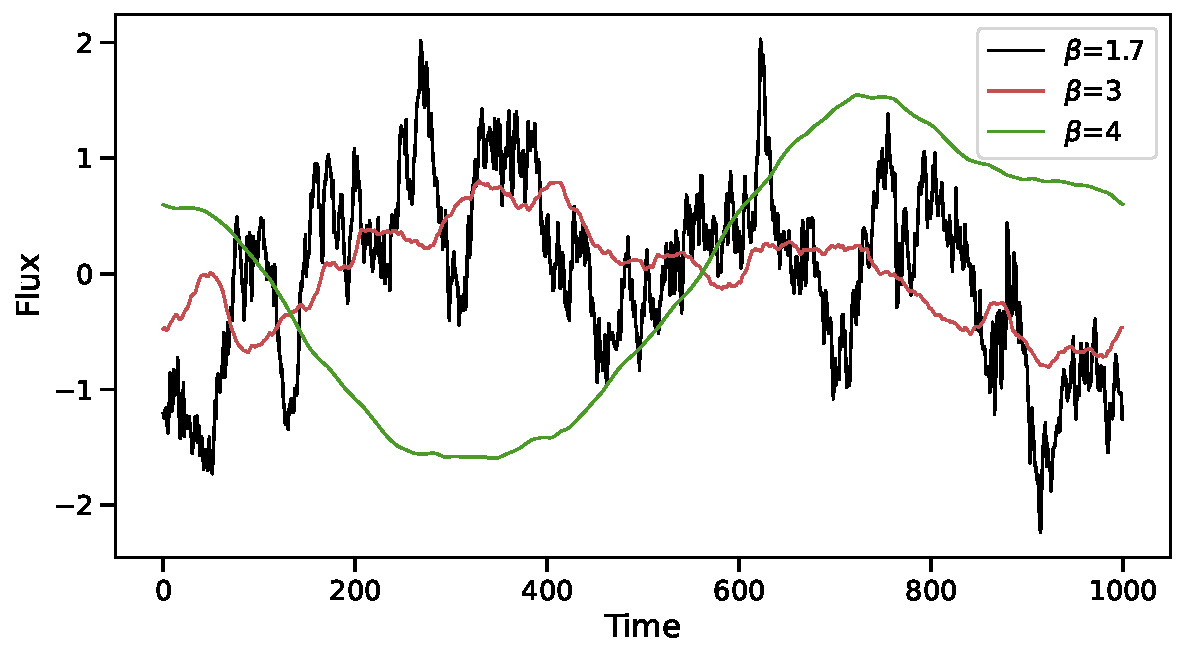
\includegraphics[width=\columnwidth]{app_A_light_curves.pdf}
                \caption{Visualisation of three light curves generated by the colorednoise code each running for 1000 time steps. In each light curve the mean flux was subtracted from the flux. The curves become progressively smoother as the power-law index increases, producing higher powers at lower frequencies in the PSD plot (see Fig. \ref{fig:app_1_2}).}
                \label{fig:app_1_1}
            \end{figure}


            \begin{figure}[h]
                \centering
                
\includegraphics[width=\columnwidth]{app_A_fig_beta_4_v2.pdf}
                \caption{PSD recovery for a colorednoise realisation with true power-law index $\beta = 4$. Black points show the unbinned periodogram of one representative AR(1) posterior draw; orange points show the same periodogram averaged into 9 logarithmically-spaced frequency bins, with error bars from the scatter within each bin. The red dashed line is the power-law-plus-constant fit (Eq.~\ref{eq:periodogram_fit}) to this single binned draw, shown for illustration; the $\beta$ value reported in Table~\ref{tab:appendix_params} is the median (with 5\%-95\% interval) over the distribution of such fits across all posterior draws, not this one realisation. The solid blue curve shows the periodogram of the true, pre-AR(1) colorednoise input signal, for direct visual comparison against the recovered fit.}
                \label{fig:app_1_2}
            \end{figure}
To test our model's ability to recover the true power-law index despite the AR(1) prior imposed by our state-space formulation, we generated synthetic red-noise light curves with known PSD slopes $\beta = 1.7$, 3, and 4 (see Fig. \ref{fig:app_1_1}), using \texttt{colorednoise}\footnote{\url{https://github.com/felixpatzelt/colorednoise}}, which implements the algorithm of \citet{TimmerKoenig1995} to generate Gaussian noise with a power spectrum $\propto f^{-\beta}$. We then modelled the statistical properties of these light curves using an AR(1) process, estimated the PSD of the resulting modelled processes using a periodogram estimator, and fit the estimated periodogram with a curve of the form:
            \begin{equation}
            \log(P) = \log\left(a f^{-\beta} + c\right)
            \end{equation}
where \( P \) is the power, \( a \) is the coefficient, \( \beta \) is the power-law index, and \( c \) is a constant that sets the noise floor (plateau) the PSD approaches at high frequency (see Fig. \ref{fig:app_1_2}). The most direct approach would be to fit this curve to the unbinned periodogram; however, this does not yield an accurate fit because periodograms follow a chi-square distribution with two degrees of freedom at a given frequency (see \citealt{BarretVaughan2012}). Binning the frequencies into 9 coarser, logarithmically-spaced segments (following \citealt{Vaughan2003}) yields a more reliable fit. We fit each periodogram using \texttt{curve\_fit} from \texttt{scipy.optimize}; the true power-law index falls outside the recovered [5\%-95\%] credible interval for all three cases (see Table~\ref{tab:appendix_params}), consistent with realisation-to-realisation scatter in the periodogram estimator rather than a systematic bias for $\beta = 1.7$, and, for $\beta = 3$ and $\beta = 4$, a systematic bias of the periodogram fit itself. Both recovered values (2.48 and 3.86) exceed the AR(1) process's asymptotic PSD slope of 2, so that ceiling does not bound them. The bias arises instead from the limited dynamic range available to the fit: the high-frequency end of the periodogram is flattened by the Poisson noise floor and by spectral leakage through the finite observing window (see Sect.~\ref{sec:verification_results_psd}), which caps the steepest slope measurable across the 9 logarithmic bins \citep[see][Sect.~4.1.2]{Kankkunen2025}. Because this fit is repeated independently for every posterior draw rather than once on a single representative trajectory, the resulting spread across draws is itself a direct, model-based estimate of the uncertainty on the recovered power-law index, obtained at no additional computational cost beyond the state-space inference already performed for other purposes.            

            \begin{table}[h]
                \caption{Parameter estimates and true values for three single realisations. The quoted [5\%--95\%] interval is the spread of $\beta$ across posterior draws of \emph{one} realisation, and therefore does not include the scatter \emph{between} independent realisations, which is substantially larger (Table~\ref{tab:beta_N40_ensemble}).}
                \centering
                \begin{tabular}{lcccc}
                \hline\hline
                Parameter & 5\% & Median & 95\% & True Value \\
                \hline
                $\beta_1$ & 1.587 & 1.591 & 1.595 & 1.70 \\
                $\beta_2$ & 2.44 & 2.48 & 2.51 & 3.00 \\
                $\beta_3$ & 3.73 & 3.86 & 3.92 & 4.00 \\
                \hline
                \end{tabular}
                \label{tab:appendix_params}
            \end{table}
The constant $c$ is retained in Eq.~\ref{eq:periodogram_fit} to capture the flattening of the PSD at high frequencies, where Poisson counting noise and red-noise leakage from the AR(1) process dominate over the power-law component; omitting it biases the recovered $\beta$ toward flatter values (see Sect.~\ref{sec:verification_results_psd}). \\
To test whether the $\tau$-pinning-at-the-prior-edge behaviour described in Sect.~\ref{sec:limitation} could be resolved by lowering the Poisson noise floor (the $c$ term above) relative to the true \texttt{colorednoise} signal, we repeated the $\beta = 3$ and $\beta = 4$ validation at increasing source count rates. Table~\ref{tab:beta34_snr_sweep} shows that as source counts increase, the posterior mean of $\tau$ moves closer to the prior's upper edge (80), for both $\beta$ values. If this pinning behaviour were simply an artefact of the Poisson floor obscuring the underlying \texttt{colorednoise} variability, reducing it relative to the signal should instead move $\tau$ away from the edge, not toward it. Higher count rates than those shown could not be reliably sampled and are therefore excluded.

            \begin{table}[h]
                \caption{Posterior mean $\tau$ as a function of average source count, for $\beta=3$ and $\beta=4$.}
                \centering
                \begin{tabular}{cccc}
                \hline\hline
                $\beta$ & avg. count & $\hat\tau$ mean & $\hat\tau$ std \\
                \hline
                3 & 4.2 & 75.68 & 4.01 \\
                3 & 77.3 & 78.45 & 1.40 \\
                3 & 1341.4 & 79.08 & 0.92 \\
                4 & 5.4 & 77.36 & 2.58 \\
                4 & 139.3 & 79.26 & 0.71 \\
                4 & 2762.4 & 79.72 & 0.27 \\
                \hline
                \end{tabular}
                \label{tab:beta34_snr_sweep}
            \end{table}
To test whether these two failure modes persist under a larger ensemble, we repeated the validation for all three $\beta$ values using $N=40$ independent realisations each. Table~\ref{tab:beta_N40_ensemble} summarises the result. $\beta=1.7$ remains unbiased (24/40 realisations below the true value, consistent with random scatter); $\beta=3$ shows weaker, intermediate evidence of bias (26/40 below true); $\beta=4$'s bias is confirmed with overwhelming statistical force (40/40 realisations below true). A steeper case ($\beta=8$) was also attempted, but at that steepness the amplitude in Eq.~\ref{eq:periodogram_fit} falls below the range our fit permits and the optimiser does not converge reliably; we therefore do not report it. Separately from the recovery bias discussed here, the AR(1) asymptotic slope of 2 remains a genuine constraint on what the \emph{model} can represent: recent ensemble PSD studies of real quasar variability find high-frequency slopes steeper than $-2$ (e.g. $-2.7\pm0.1$ across a large Stripe-82 quasar sample in the UV; \citealt{Petrecca2026}), so this limitation is not confined to synthetic data. This value falls close to our own $\beta=3$ case, where the recovered bias is comparatively mild (mean $2.87$, only marginal statistical evidence of bias; Table~\ref{tab:beta_N40_ensemble}); the severe, overwhelming bias we identify only becomes unambiguous for steeper processes ($\beta\gtrsim4$), beyond what \citet{Petrecca2026} report for this population. \\

            \begin{table}[h]
                \caption{$N=40$ realisation-ensemble mean recovered $\beta$ (a separate, larger test from Table~\ref{tab:appendix_params}, not directly comparable to it row-for-row).}
                \centering
                \begin{tabular}{cccc}
                \hline\hline
                True $\beta$ & Mean & Std & Below true/N \\
                \hline
                1.7 & 1.67 & 0.17 & 24/40 \\
                3.0 & 2.87 & 0.28 & 26/40 \\
                4.0 & 3.54 & 0.24 & 40/40 \\
                \hline
                \end{tabular}
                \tablefoot{Mean and standard deviation are taken across the 40 per-realisation median $\beta$ values; the quoted standard deviation is realisation-to-realisation scatter, not the posterior uncertainty within a single realisation.}
                \label{tab:beta_N40_ensemble}
            \end{table}


\section{Intrinsic absorption behaviour for different values of $N_H$}
\label{app:optical_depth}

To make explicit the sensitivity threshold invoked in Sect.~\ref{sec:verification_results_parameter} to explain the systematic underestimation of $N_H$ at low column density, Fig.~\ref{fig:nh_flux_threshold} compares the intrinsically absorbed power-law flux for four values of $N_H$ spanning $10^{10}$--$10^{21}$\,cm$^{-2}$. Below $N_H \sim 10^{20}$\,cm$^{-2}$ the absorbed spectra are visually indistinguishable from the unabsorbed case across the observed bandpass, confirming the data carry essentially no information to constrain $N_H$ in this regime; only at $N_H = 10^{21}$\,cm$^{-2}$ does soft-band suppression become detectable.

\begin{figure}[htbp]
\centering
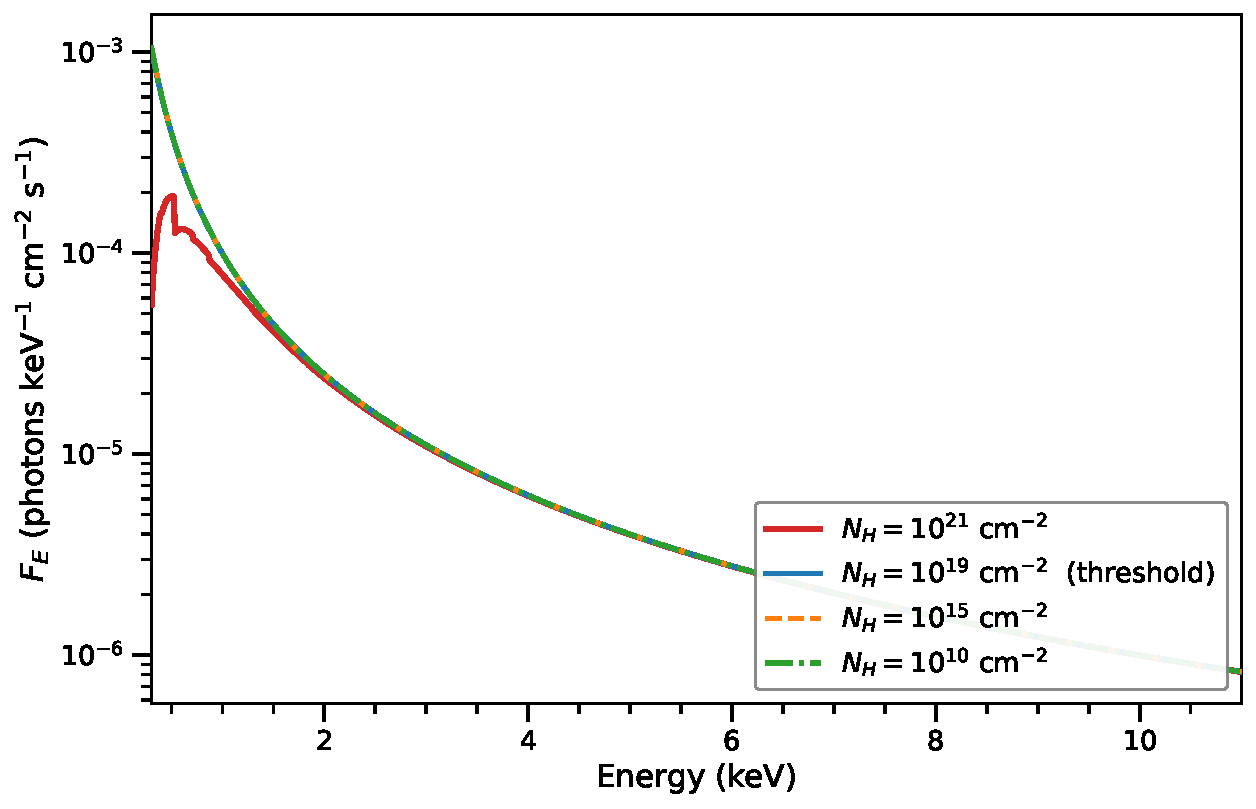
\includegraphics[width=\columnwidth]{observed_flux_NH_comparison.pdf}
\caption{Intrinsic absorbed power-law flux $F_E$ as a function of 
photon energy for four values of hydrogen column density $N_H$, 
illustrating the effective sensitivity threshold of X-ray 
photoelectric absorption. The spectral model is a power law with 
photon index $\Gamma = 2.0$ and normalisation $K = 10^{-4}$, 
attenuated by $\exp(-N_H\,\sigma(E))$, where $\sigma(E)$ is the 
photoelectric absorption cross-section from 
\citet{wilms2000}. No Galactic foreground absorption is included; 
all curves represent intrinsic absorption at the source in the 
rest frame ($z = 0$). The three curves for $N_H = 10^{10}$, 
$10^{15}$, and $10^{19}$\,cm$^{-2}$ are indistinguishable from 
one another across the full energy range, demonstrating that below 
$N_H \sim 10^{20}$\,cm$^{-2}$ the attenuation factor 
$e^{-N_H\sigma(E)} \approx 1$ and the spectrum carries essentially 
no information about $N_H$. Only at $N_H = 10^{21}$\,cm$^{-2}$ 
does the soft-band ($E \lesssim 1$\,keV) suppression become 
detectable. This defines the lower sensitivity boundary of our 
inference framework and explains the systematic underestimation of 
$N_H$ observed in simulations with true $N_H = 10^{19}$\,cm$^{-2}$ 
(Table~\ref{tab:light_curve_sim_table}).}
\label{fig:nh_flux_threshold}
\end{figure}
 


%%%% End of aa.dem
\end{document}
